\documentclass[twoside]{book}

% Packages required by doxygen
\usepackage{fixltx2e}
\usepackage{calc}
\usepackage{doxygen}
\usepackage[export]{adjustbox} % also loads graphicx
\usepackage{graphicx}
\usepackage[utf8]{inputenc}
\usepackage{makeidx}
\usepackage{multicol}
\usepackage{multirow}
\PassOptionsToPackage{warn}{textcomp}
\usepackage{textcomp}
\usepackage[nointegrals]{wasysym}
\usepackage[table]{xcolor}

% Font selection
\usepackage[T1]{fontenc}
\usepackage[scaled=.90]{helvet}
\usepackage{courier}
\usepackage{amssymb}
\usepackage{sectsty}
\renewcommand{\familydefault}{\sfdefault}
\allsectionsfont{%
  \fontseries{bc}\selectfont%
  \color{darkgray}%
}
\renewcommand{\DoxyLabelFont}{%
  \fontseries{bc}\selectfont%
  \color{darkgray}%
}
\newcommand{\+}{\discretionary{\mbox{\scriptsize$\hookleftarrow$}}{}{}}

% Page & text layout
\usepackage{geometry}
\geometry{%
  a4paper,%
  top=2.5cm,%
  bottom=2.5cm,%
  left=2.5cm,%
  right=2.5cm%
}
\tolerance=750
\hfuzz=15pt
\hbadness=750
\setlength{\emergencystretch}{15pt}
\setlength{\parindent}{0cm}
\setlength{\parskip}{3ex plus 2ex minus 2ex}
\makeatletter
\renewcommand{\paragraph}{%
  \@startsection{paragraph}{4}{0ex}{-1.0ex}{1.0ex}{%
    \normalfont\normalsize\bfseries\SS@parafont%
  }%
}
\renewcommand{\subparagraph}{%
  \@startsection{subparagraph}{5}{0ex}{-1.0ex}{1.0ex}{%
    \normalfont\normalsize\bfseries\SS@subparafont%
  }%
}
\makeatother

% Headers & footers
\usepackage{fancyhdr}
\pagestyle{fancyplain}
\fancyhead[LE]{\fancyplain{}{\bfseries\thepage}}
\fancyhead[CE]{\fancyplain{}{}}
\fancyhead[RE]{\fancyplain{}{\bfseries\leftmark}}
\fancyhead[LO]{\fancyplain{}{\bfseries\rightmark}}
\fancyhead[CO]{\fancyplain{}{}}
\fancyhead[RO]{\fancyplain{}{\bfseries\thepage}}
\fancyfoot[LE]{\fancyplain{}{}}
\fancyfoot[CE]{\fancyplain{}{}}
\fancyfoot[RE]{\fancyplain{}{\bfseries\scriptsize Generated by Doxygen }}
\fancyfoot[LO]{\fancyplain{}{\bfseries\scriptsize Generated by Doxygen }}
\fancyfoot[CO]{\fancyplain{}{}}
\fancyfoot[RO]{\fancyplain{}{}}
\renewcommand{\footrulewidth}{0.4pt}
\renewcommand{\chaptermark}[1]{%
  \markboth{#1}{}%
}
\renewcommand{\sectionmark}[1]{%
  \markright{\thesection\ #1}%
}

% Indices & bibliography
\usepackage{natbib}
\usepackage[titles]{tocloft}
\setcounter{tocdepth}{3}
\setcounter{secnumdepth}{5}
\makeindex

% Hyperlinks (required, but should be loaded last)
\usepackage{ifpdf}
\ifpdf
  \usepackage[pdftex,pagebackref=true]{hyperref}
\else
  \usepackage[ps2pdf,pagebackref=true]{hyperref}
\fi
\hypersetup{%
  colorlinks=true,%
  linkcolor=blue,%
  citecolor=blue,%
  unicode%
}

% Custom commands
\newcommand{\clearemptydoublepage}{%
  \newpage{\pagestyle{empty}\cleardoublepage}%
}

\usepackage{caption}
\captionsetup{labelsep=space,justification=centering,font={bf},singlelinecheck=off,skip=4pt,position=top}

%===== C O N T E N T S =====

\begin{document}

% Titlepage & ToC
\hypersetup{pageanchor=false,
             bookmarksnumbered=true,
             pdfencoding=unicode
            }
\pagenumbering{alph}
\begin{titlepage}
\vspace*{7cm}
\begin{center}%
{\Large A\+D\+AS M\+CU \\[1ex]\large v1.\+0 }\\
\vspace*{1cm}
{\large Generated by Doxygen 1.8.14}\\
\end{center}
\end{titlepage}
\clearemptydoublepage
\pagenumbering{roman}
\tableofcontents
\clearemptydoublepage
\pagenumbering{arabic}
\hypersetup{pageanchor=true}

%--- Begin generated contents ---
\chapter{Description}
\label{index}\hypertarget{index}{}This is the documentation of the Motor Contol Unit (M\+CU) of the A\+D\+AS project. 
\chapter{Class Index}
\section{Class List}
Here are the classes, structs, unions and interfaces with brief descriptions\+:\begin{DoxyCompactList}
\item\contentsline{section}{\mbox{\hyperlink{class_c_a_d_c}{C\+A\+DC}} }{\pageref{class_c_a_d_c}}{}
\item\contentsline{section}{\mbox{\hyperlink{class_c_buff_adas}{C\+Buff\+Adas}} }{\pageref{class_c_buff_adas}}{}
\item\contentsline{section}{\mbox{\hyperlink{class_c_environmental_data}{C\+Environmental\+Data}} }{\pageref{class_c_environmental_data}}{}
\item\contentsline{section}{\mbox{\hyperlink{class_c_i_c_c_comms}{C\+I\+C\+C\+Comms}} }{\pageref{class_c_i_c_c_comms}}{}
\item\contentsline{section}{\mbox{\hyperlink{class_c_navigation}{C\+Navigation}} }{\pageref{class_c_navigation}}{}
\item\contentsline{section}{\mbox{\hyperlink{class_c_p_l_s_comms}{C\+P\+L\+S\+Comms}} }{\pageref{class_c_p_l_s_comms}}{}
\item\contentsline{section}{\mbox{\hyperlink{class_c_positioning}{C\+Positioning}} }{\pageref{class_c_positioning}}{}
\item\contentsline{section}{\mbox{\hyperlink{class_c_serial}{C\+Serial}} }{\pageref{class_c_serial}}{}
\item\contentsline{section}{\mbox{\hyperlink{class_c_task_ctrl}{C\+Task\+Ctrl}} }{\pageref{class_c_task_ctrl}}{}
\item\contentsline{section}{\mbox{\hyperlink{class_c_user___i_f}{C\+User\+\_\+\+IF}} }{\pageref{class_c_user___i_f}}{}
\item\contentsline{section}{\mbox{\hyperlink{class_c_v_mapping}{C\+V\+Mapping}} }{\pageref{class_c_v_mapping}}{}
\item\contentsline{section}{\mbox{\hyperlink{class_i_task___i_f}{I\+Task\+\_\+\+IF}} }{\pageref{class_i_task___i_f}}{}
\item\contentsline{section}{\mbox{\hyperlink{struct_c_i_c_c_comms_1_1_message__t}{C\+I\+C\+C\+Comms\+::\+Message\+\_\+t}} }{\pageref{struct_c_i_c_c_comms_1_1_message__t}}{}
\item\contentsline{section}{\mbox{\hyperlink{struct_c_p_l_s_comms_1_1_message__t}{C\+P\+L\+S\+Comms\+::\+Message\+\_\+t}} }{\pageref{struct_c_p_l_s_comms_1_1_message__t}}{}
\end{DoxyCompactList}

\chapter{File Index}
\section{File List}
Here is a list of all files with brief descriptions\+:\begin{DoxyCompactList}
\item\contentsline{section}{\mbox{\hyperlink{_a_d_a_s___cfg_8h}{A\+D\+A\+S\+\_\+\+Cfg.\+h}} \\*This file contains the configuration of the vehicle }{\pageref{_a_d_a_s___cfg_8h}}{}
\item\contentsline{section}{\mbox{\hyperlink{_a_d_a_s___debug_8h}{A\+D\+A\+S\+\_\+\+Debug.\+h}} \\*This file contains redefinition of the serial functions for debugging purpose }{\pageref{_a_d_a_s___debug_8h}}{}
\item\contentsline{section}{\mbox{\hyperlink{_a_d_a_s___nav_u_8ino}{A\+D\+A\+S\+\_\+\+Nav\+U.\+ino}} \\*Main file for the NavU of the A\+D\+AS project }{\pageref{_a_d_a_s___nav_u_8ino}}{}
\item\contentsline{section}{\mbox{\hyperlink{_a_d_a_s___types_8h}{A\+D\+A\+S\+\_\+\+Types.\+h}} }{\pageref{_a_d_a_s___types_8h}}{}
\item\contentsline{section}{\mbox{\hyperlink{_app___environmental_data_8cpp}{App\+\_\+\+Environmental\+Data.\+cpp}} \\*Application file for environmental data }{\pageref{_app___environmental_data_8cpp}}{}
\item\contentsline{section}{\mbox{\hyperlink{_app___environmental_data_8h}{App\+\_\+\+Environmental\+Data.\+h}} \\*Application file for environmental data }{\pageref{_app___environmental_data_8h}}{}
\item\contentsline{section}{\mbox{\hyperlink{_app___navigation_8cpp}{App\+\_\+\+Navigation.\+cpp}} \\*Application file for navigation }{\pageref{_app___navigation_8cpp}}{}
\item\contentsline{section}{\mbox{\hyperlink{_app___navigation_8h}{App\+\_\+\+Navigation.\+h}} \\*Application file for navigation }{\pageref{_app___navigation_8h}}{}
\item\contentsline{section}{\mbox{\hyperlink{_app___positioning_8cpp}{App\+\_\+\+Positioning.\+cpp}} }{\pageref{_app___positioning_8cpp}}{}
\item\contentsline{section}{\mbox{\hyperlink{_app___positioning_8h}{App\+\_\+\+Positioning.\+h}} }{\pageref{_app___positioning_8h}}{}
\item\contentsline{section}{\mbox{\hyperlink{_app___user_interface_8cpp}{App\+\_\+\+User\+Interface.\+cpp}} }{\pageref{_app___user_interface_8cpp}}{}
\item\contentsline{section}{\mbox{\hyperlink{_app___user_interface_8h}{App\+\_\+\+User\+Interface.\+h}} }{\pageref{_app___user_interface_8h}}{}
\item\contentsline{section}{\mbox{\hyperlink{_app___virtual_mapping_8cpp}{App\+\_\+\+Virtual\+Mapping.\+cpp}} }{\pageref{_app___virtual_mapping_8cpp}}{}
\item\contentsline{section}{\mbox{\hyperlink{_app___virtual_mapping_8h}{App\+\_\+\+Virtual\+Mapping.\+h}} }{\pageref{_app___virtual_mapping_8h}}{}
\item\contentsline{section}{\mbox{\hyperlink{_cbuffer_8cpp}{Cbuffer.\+cpp}} }{\pageref{_cbuffer_8cpp}}{}
\item\contentsline{section}{\mbox{\hyperlink{_cbuffer_8h}{Cbuffer.\+h}} }{\pageref{_cbuffer_8h}}{}
\item\contentsline{section}{\mbox{\hyperlink{_comm___i_c_c_8cpp}{Comm\+\_\+\+I\+C\+C.\+cpp}} \\*Communication file for Inter-\/\+Controller Communication (I\+CC) }{\pageref{_comm___i_c_c_8cpp}}{}
\item\contentsline{section}{\mbox{\hyperlink{_comm___i_c_c_8h}{Comm\+\_\+\+I\+C\+C.\+h}} \\*Communication file for Inter-\/\+Controller Communication (I\+CC) }{\pageref{_comm___i_c_c_8h}}{}
\item\contentsline{section}{\mbox{\hyperlink{_comm___p_l_s_8cpp}{Comm\+\_\+\+P\+L\+S.\+cpp}} }{\pageref{_comm___p_l_s_8cpp}}{}
\item\contentsline{section}{\mbox{\hyperlink{_comm___p_l_s_8h}{Comm\+\_\+\+P\+L\+S.\+h}} }{\pageref{_comm___p_l_s_8h}}{}
\item\contentsline{section}{\mbox{\hyperlink{_h_a_l___a_d_c_8cpp}{H\+A\+L\+\_\+\+A\+D\+C.\+cpp}} \\*Hardware Abstraction Layer (H\+AL) to interface A\+DC }{\pageref{_h_a_l___a_d_c_8cpp}}{}
\item\contentsline{section}{\mbox{\hyperlink{_h_a_l___a_d_c_8h}{H\+A\+L\+\_\+\+A\+D\+C.\+h}} \\*Hardware Abstraction Layer (H\+AL) to interface A\+DC }{\pageref{_h_a_l___a_d_c_8h}}{}
\item\contentsline{section}{\mbox{\hyperlink{_h_a_l___p_w_m_8cpp}{H\+A\+L\+\_\+\+P\+W\+M.\+cpp}} \\*Hardware Abstraction Layer (H\+AL) for the 10-\/bit P\+WM outputs }{\pageref{_h_a_l___p_w_m_8cpp}}{}
\item\contentsline{section}{\mbox{\hyperlink{_h_a_l___p_w_m_8h}{H\+A\+L\+\_\+\+P\+W\+M.\+h}} \\*Hardware Abstraction Layer (H\+AL) for the 10-\/bit P\+WM outputs }{\pageref{_h_a_l___p_w_m_8h}}{}
\item\contentsline{section}{\mbox{\hyperlink{_h_a_l___serial___i_f_8cpp}{H\+A\+L\+\_\+\+Serial\+\_\+\+I\+F.\+cpp}} \\*Hardware Abstraction Layer (H\+AL) to serial interface }{\pageref{_h_a_l___serial___i_f_8cpp}}{}
\item\contentsline{section}{\mbox{\hyperlink{_h_a_l___serial___i_f_8h}{H\+A\+L\+\_\+\+Serial\+\_\+\+I\+F.\+h}} \\*Hardware Abstraction Layer (H\+AL) to serial interface }{\pageref{_h_a_l___serial___i_f_8h}}{}
\item\contentsline{section}{\mbox{\hyperlink{_o_s_a_l___task_ctrl_8cpp}{O\+S\+A\+L\+\_\+\+Task\+Ctrl.\+cpp}} }{\pageref{_o_s_a_l___task_ctrl_8cpp}}{}
\item\contentsline{section}{\mbox{\hyperlink{_o_s_a_l___task_ctrl_8h}{O\+S\+A\+L\+\_\+\+Task\+Ctrl.\+h}} }{\pageref{_o_s_a_l___task_ctrl_8h}}{}
\item\contentsline{section}{\mbox{\hyperlink{_task___i_f_8h}{Task\+\_\+\+I\+F.\+h}} }{\pageref{_task___i_f_8h}}{}
\end{DoxyCompactList}

\chapter{Class Documentation}
\hypertarget{class_c_buff_adas}{}\section{C\+Buff\+Adas Class Reference}
\label{class_c_buff_adas}\index{C\+Buff\+Adas@{C\+Buff\+Adas}}


{\ttfamily \#include $<$Cbuffer.\+h$>$}



Collaboration diagram for C\+Buff\+Adas\+:
\nopagebreak
\begin{figure}[H]
\begin{center}
\leavevmode
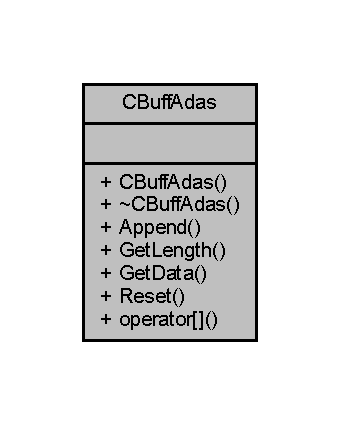
\includegraphics[width=163pt]{class_c_buff_adas__coll__graph}
\end{center}
\end{figure}
\subsection*{Public Member Functions}
\begin{DoxyCompactItemize}
\item 
\mbox{\hyperlink{class_c_buff_adas_a7491e123b003457b2565435ae7ac9ce4}{C\+Buff\+Adas}} (\mbox{\hyperlink{_a_d_a_s___types_8h_aba7bc1797add20fe3efdf37ced1182c5}{uint8\+\_\+t}} $\ast$data, const \mbox{\hyperlink{_a_d_a_s___types_8h_a1f1825b69244eb3ad2c7165ddc99c956}{uint16\+\_\+t}} len)
\begin{DoxyCompactList}\small\item\em Cbuffer constructor. \end{DoxyCompactList}\item 
\mbox{\hyperlink{class_c_buff_adas_a55af513577ba8522492fff4db85da247}{$\sim$\+C\+Buff\+Adas}} ()
\begin{DoxyCompactList}\small\item\em Cbuffer destructor. \end{DoxyCompactList}\item 
void \mbox{\hyperlink{class_c_buff_adas_aceac4b71872e406861286959f578c89b}{Append}} (const \mbox{\hyperlink{_a_d_a_s___types_8h_aba7bc1797add20fe3efdf37ced1182c5}{uint8\+\_\+t}} data)
\begin{DoxyCompactList}\small\item\em Append data. \end{DoxyCompactList}\item 
\mbox{\hyperlink{_a_d_a_s___types_8h_a1f1825b69244eb3ad2c7165ddc99c956}{uint16\+\_\+t}} \mbox{\hyperlink{class_c_buff_adas_a493f61488df8ac9f7e942af1a2fbdbf3}{Get\+Length}} ()
\begin{DoxyCompactList}\small\item\em get lenght \end{DoxyCompactList}\item 
\mbox{\hyperlink{_a_d_a_s___types_8h_aba7bc1797add20fe3efdf37ced1182c5}{uint8\+\_\+t}} $\ast$ \mbox{\hyperlink{class_c_buff_adas_a56fdcdc9766874d3a6fef04119ee91f9}{Get\+Data}} ()
\begin{DoxyCompactList}\small\item\em get buffer pointer \end{DoxyCompactList}\item 
void \mbox{\hyperlink{class_c_buff_adas_a2ff1ee5f1dfa56117d76b17027d7b7e8}{Reset}} ()
\begin{DoxyCompactList}\small\item\em reset buffer \end{DoxyCompactList}\item 
\mbox{\hyperlink{_a_d_a_s___types_8h_a06896e8c53f721507066c079052171f8}{uint32\+\_\+t}} \mbox{\hyperlink{class_c_buff_adas_ae1a6aa5f049b0e1e04950af1c55df3d7}{operator\mbox{[}$\,$\mbox{]}}} (const \mbox{\hyperlink{_a_d_a_s___types_8h_a06896e8c53f721507066c079052171f8}{uint32\+\_\+t}} index)
\begin{DoxyCompactList}\small\item\em operator overloading \mbox{[}\mbox{]} \end{DoxyCompactList}\end{DoxyCompactItemize}


\subsection{Detailed Description}


Definition at line 13 of file Cbuffer.\+h.



\subsection{Constructor \& Destructor Documentation}
\mbox{\Hypertarget{class_c_buff_adas_a7491e123b003457b2565435ae7ac9ce4}\label{class_c_buff_adas_a7491e123b003457b2565435ae7ac9ce4}} 
\index{C\+Buff\+Adas@{C\+Buff\+Adas}!C\+Buff\+Adas@{C\+Buff\+Adas}}
\index{C\+Buff\+Adas@{C\+Buff\+Adas}!C\+Buff\+Adas@{C\+Buff\+Adas}}
\subsubsection{\texorpdfstring{C\+Buff\+Adas()}{CBuffAdas()}}
{\footnotesize\ttfamily C\+Buff\+Adas\+::\+C\+Buff\+Adas (\begin{DoxyParamCaption}\item[{\mbox{\hyperlink{_a_d_a_s___types_8h_aba7bc1797add20fe3efdf37ced1182c5}{uint8\+\_\+t}} $\ast$}]{data,  }\item[{const \mbox{\hyperlink{_a_d_a_s___types_8h_a1f1825b69244eb3ad2c7165ddc99c956}{uint16\+\_\+t}}}]{len }\end{DoxyParamCaption})}



Cbuffer constructor. 

Instantiation and initialization 
\begin{DoxyParams}[1]{Parameters}
\mbox{\tt in}  & {\em data} & buffer memory pointer \\
\hline
\mbox{\tt in}  & {\em len} & length of buffer memory \\
\hline
\end{DoxyParams}


Definition at line 4 of file Cbuffer.\+cpp.

\mbox{\Hypertarget{class_c_buff_adas_a55af513577ba8522492fff4db85da247}\label{class_c_buff_adas_a55af513577ba8522492fff4db85da247}} 
\index{C\+Buff\+Adas@{C\+Buff\+Adas}!````~C\+Buff\+Adas@{$\sim$\+C\+Buff\+Adas}}
\index{````~C\+Buff\+Adas@{$\sim$\+C\+Buff\+Adas}!C\+Buff\+Adas@{C\+Buff\+Adas}}
\subsubsection{\texorpdfstring{$\sim$\+C\+Buff\+Adas()}{~CBuffAdas()}}
{\footnotesize\ttfamily C\+Buff\+Adas\+::$\sim$\+C\+Buff\+Adas (\begin{DoxyParamCaption}{ }\end{DoxyParamCaption})}



Cbuffer destructor. 



Definition at line 12 of file Cbuffer.\+cpp.



\subsection{Member Function Documentation}
\mbox{\Hypertarget{class_c_buff_adas_aceac4b71872e406861286959f578c89b}\label{class_c_buff_adas_aceac4b71872e406861286959f578c89b}} 
\index{C\+Buff\+Adas@{C\+Buff\+Adas}!Append@{Append}}
\index{Append@{Append}!C\+Buff\+Adas@{C\+Buff\+Adas}}
\subsubsection{\texorpdfstring{Append()}{Append()}}
{\footnotesize\ttfamily void C\+Buff\+Adas\+::\+Append (\begin{DoxyParamCaption}\item[{const \mbox{\hyperlink{_a_d_a_s___types_8h_aba7bc1797add20fe3efdf37ced1182c5}{uint8\+\_\+t}}}]{data }\end{DoxyParamCaption})}



Append data. 


\begin{DoxyParams}[1]{Parameters}
\mbox{\tt in}  & {\em data} & byte to be appended \\
\hline
\end{DoxyParams}


Definition at line 18 of file Cbuffer.\+cpp.

\mbox{\Hypertarget{class_c_buff_adas_a56fdcdc9766874d3a6fef04119ee91f9}\label{class_c_buff_adas_a56fdcdc9766874d3a6fef04119ee91f9}} 
\index{C\+Buff\+Adas@{C\+Buff\+Adas}!Get\+Data@{Get\+Data}}
\index{Get\+Data@{Get\+Data}!C\+Buff\+Adas@{C\+Buff\+Adas}}
\subsubsection{\texorpdfstring{Get\+Data()}{GetData()}}
{\footnotesize\ttfamily \mbox{\hyperlink{_a_d_a_s___types_8h_aba7bc1797add20fe3efdf37ced1182c5}{uint8\+\_\+t}} $\ast$ C\+Buff\+Adas\+::\+Get\+Data (\begin{DoxyParamCaption}{ }\end{DoxyParamCaption})}



get buffer pointer 

\begin{DoxyReturn}{Returns}
pointer to buffer 
\end{DoxyReturn}


Definition at line 31 of file Cbuffer.\+cpp.

\mbox{\Hypertarget{class_c_buff_adas_a493f61488df8ac9f7e942af1a2fbdbf3}\label{class_c_buff_adas_a493f61488df8ac9f7e942af1a2fbdbf3}} 
\index{C\+Buff\+Adas@{C\+Buff\+Adas}!Get\+Length@{Get\+Length}}
\index{Get\+Length@{Get\+Length}!C\+Buff\+Adas@{C\+Buff\+Adas}}
\subsubsection{\texorpdfstring{Get\+Length()}{GetLength()}}
{\footnotesize\ttfamily \mbox{\hyperlink{_a_d_a_s___types_8h_a1f1825b69244eb3ad2c7165ddc99c956}{uint16\+\_\+t}} C\+Buff\+Adas\+::\+Get\+Length (\begin{DoxyParamCaption}{ }\end{DoxyParamCaption})}



get lenght 

\begin{DoxyReturn}{Returns}
length of used buffer 
\end{DoxyReturn}


Definition at line 26 of file Cbuffer.\+cpp.

\mbox{\Hypertarget{class_c_buff_adas_ae1a6aa5f049b0e1e04950af1c55df3d7}\label{class_c_buff_adas_ae1a6aa5f049b0e1e04950af1c55df3d7}} 
\index{C\+Buff\+Adas@{C\+Buff\+Adas}!operator\mbox{[}\mbox{]}@{operator[]}}
\index{operator\mbox{[}\mbox{]}@{operator[]}!C\+Buff\+Adas@{C\+Buff\+Adas}}
\subsubsection{\texorpdfstring{operator[]()}{operator[]()}}
{\footnotesize\ttfamily \mbox{\hyperlink{_a_d_a_s___types_8h_a06896e8c53f721507066c079052171f8}{uint32\+\_\+t}} C\+Buff\+Adas\+::operator\mbox{[}$\,$\mbox{]} (\begin{DoxyParamCaption}\item[{const \mbox{\hyperlink{_a_d_a_s___types_8h_a06896e8c53f721507066c079052171f8}{uint32\+\_\+t}}}]{index }\end{DoxyParamCaption})}



operator overloading \mbox{[}\mbox{]} 


\begin{DoxyParams}{Parameters}
{\em index} & index \\
\hline
\end{DoxyParams}
\begin{DoxyReturn}{Returns}
uint32\+\_\+t 
\end{DoxyReturn}


Definition at line 41 of file Cbuffer.\+cpp.

\mbox{\Hypertarget{class_c_buff_adas_a2ff1ee5f1dfa56117d76b17027d7b7e8}\label{class_c_buff_adas_a2ff1ee5f1dfa56117d76b17027d7b7e8}} 
\index{C\+Buff\+Adas@{C\+Buff\+Adas}!Reset@{Reset}}
\index{Reset@{Reset}!C\+Buff\+Adas@{C\+Buff\+Adas}}
\subsubsection{\texorpdfstring{Reset()}{Reset()}}
{\footnotesize\ttfamily void C\+Buff\+Adas\+::\+Reset (\begin{DoxyParamCaption}{ }\end{DoxyParamCaption})}



reset buffer 



Definition at line 36 of file Cbuffer.\+cpp.

Here is the caller graph for this function\+:
\nopagebreak
\begin{figure}[H]
\begin{center}
\leavevmode
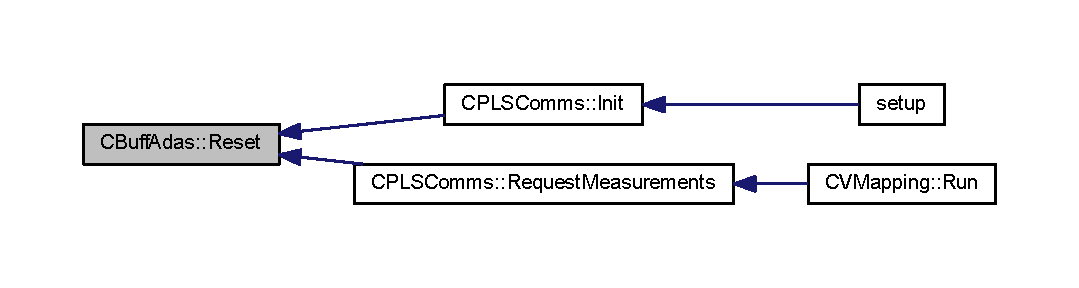
\includegraphics[width=350pt]{class_c_buff_adas_a2ff1ee5f1dfa56117d76b17027d7b7e8_icgraph}
\end{center}
\end{figure}


The documentation for this class was generated from the following files\+:\begin{DoxyCompactItemize}
\item 
\mbox{\hyperlink{_cbuffer_8h}{Cbuffer.\+h}}\item 
\mbox{\hyperlink{_cbuffer_8cpp}{Cbuffer.\+cpp}}\end{DoxyCompactItemize}

\hypertarget{class_c_drive_unit}{}\section{C\+Drive\+Unit Class Reference}
\label{class_c_drive_unit}\index{CDriveUnit@{CDriveUnit}}


{\ttfamily \#include $<$H\+A\+L\+\_\+\+Drive\+Unit.\+h$>$}



Collaboration diagram for C\+Drive\+Unit\+:
% FIG 0
\subsection*{Public Types}
\begin{DoxyCompactItemize}
\item 
enum \mbox{\hyperlink{class_c_drive_unit_a4edb3384824cee71b23c42025b689d4e}{Drive\+I\+D\+\_\+e}} \{ \mbox{\hyperlink{class_c_drive_unit_a4edb3384824cee71b23c42025b689d4ea5069438f822a5eb645aa78d8e4b461dd}{Drive1}}, 
\mbox{\hyperlink{class_c_drive_unit_a4edb3384824cee71b23c42025b689d4eaf18a8a2892d6497a0d3697e22848dfe0}{Drive2}}
 \}
\end{DoxyCompactItemize}
\subsection*{Public Member Functions}
\begin{DoxyCompactItemize}
\item 
\mbox{\hyperlink{class_c_drive_unit_aee1e28a6ee6956b8b2a01f09cfc102ee}{C\+Drive\+Unit}} (\mbox{\hyperlink{class_c_drive_unit_a4edb3384824cee71b23c42025b689d4e}{Drive\+I\+D\+\_\+e}} ID)
\item 
\mbox{\hyperlink{class_c_drive_unit_add2dcafc20d8e30ddc8ee2affb5085ee}{$\sim$\+C\+Drive\+Unit}} ()
\item 
void \mbox{\hyperlink{class_c_drive_unit_ab7b775c0f68db1490ecf8a726dbe786d}{Init}} (void)
\item 
bool \mbox{\hyperlink{class_c_drive_unit_a06ffeb71565bc8edabadae09157c705e}{Set\+Speed}} (\mbox{\hyperlink{_a_d_a_s___types_8h_aba7bc1797add20fe3efdf37ced1182c5}{uint8\+\_\+t}} speed)
\end{DoxyCompactItemize}


\subsection{Detailed Description}


Definition at line 11 of file H\+A\+L\+\_\+\+Drive\+Unit.\+h.



\subsection{Member Enumeration Documentation}
\mbox{\Hypertarget{class_c_drive_unit_a4edb3384824cee71b23c42025b689d4e}\label{class_c_drive_unit_a4edb3384824cee71b23c42025b689d4e}} 
\index{CDriveUnit@{CDriveUnit}!DriveID\_e@{DriveID\_e}}
\index{DriveID\_e@{DriveID\_e}!CDriveUnit@{CDriveUnit}}
\subsubsection{\texorpdfstring{DriveID\_e}{DriveID\_e}}
{\footnotesize\ttfamily enum \mbox{\hyperlink{class_c_drive_unit_a4edb3384824cee71b23c42025b689d4e}{C\+Drive\+Unit\+::\+Drive\+I\+D\+\_\+e}}}

\begin{DoxyEnumFields}{Enumerator}
\raisebox{\heightof{T}}[0pt][0pt]{\index{Drive1@{Drive1}!CDriveUnit@{CDriveUnit}}\index{CDriveUnit@{CDriveUnit}!Drive1@{Drive1}}}\mbox{\Hypertarget{class_c_drive_unit_a4edb3384824cee71b23c42025b689d4ea5069438f822a5eb645aa78d8e4b461dd}\label{class_c_drive_unit_a4edb3384824cee71b23c42025b689d4ea5069438f822a5eb645aa78d8e4b461dd}} 
Drive1&\\
\hline

\raisebox{\heightof{T}}[0pt][0pt]{\index{Drive2@{Drive2}!CDriveUnit@{CDriveUnit}}\index{CDriveUnit@{CDriveUnit}!Drive2@{Drive2}}}\mbox{\Hypertarget{class_c_drive_unit_a4edb3384824cee71b23c42025b689d4eaf18a8a2892d6497a0d3697e22848dfe0}\label{class_c_drive_unit_a4edb3384824cee71b23c42025b689d4eaf18a8a2892d6497a0d3697e22848dfe0}} 
Drive2&\\
\hline

\end{DoxyEnumFields}


Definition at line 13 of file H\+A\+L\+\_\+\+Drive\+Unit.\+h.



\subsection{Constructor \& Destructor Documentation}
\mbox{\Hypertarget{class_c_drive_unit_aee1e28a6ee6956b8b2a01f09cfc102ee}\label{class_c_drive_unit_aee1e28a6ee6956b8b2a01f09cfc102ee}} 
\index{CDriveUnit@{CDriveUnit}!CDriveUnit@{CDriveUnit}}
\index{CDriveUnit@{CDriveUnit}!CDriveUnit@{CDriveUnit}}
\subsubsection{\texorpdfstring{CDriveUnit()}{CDriveUnit()}}
{\footnotesize\ttfamily C\+Drive\+Unit\+::\+C\+Drive\+Unit (\begin{DoxyParamCaption}\item[{\mbox{\hyperlink{class_c_drive_unit_a4edb3384824cee71b23c42025b689d4e}{Drive\+I\+D\+\_\+e}}}]{ID }\end{DoxyParamCaption})}



Definition at line 4 of file H\+A\+L\+\_\+\+Drive\+Unit.\+cpp.

\mbox{\Hypertarget{class_c_drive_unit_add2dcafc20d8e30ddc8ee2affb5085ee}\label{class_c_drive_unit_add2dcafc20d8e30ddc8ee2affb5085ee}} 
\index{CDriveUnit@{CDriveUnit}!````~CDriveUnit@{$\sim$CDriveUnit}}
\index{````~CDriveUnit@{$\sim$CDriveUnit}!CDriveUnit@{CDriveUnit}}
\subsubsection{\texorpdfstring{$\sim$CDriveUnit()}{~CDriveUnit()}}
{\footnotesize\ttfamily C\+Drive\+Unit\+::$\sim$\+C\+Drive\+Unit (\begin{DoxyParamCaption}{ }\end{DoxyParamCaption})}



Definition at line 9 of file H\+A\+L\+\_\+\+Drive\+Unit.\+cpp.



\subsection{Member Function Documentation}
\mbox{\Hypertarget{class_c_drive_unit_ab7b775c0f68db1490ecf8a726dbe786d}\label{class_c_drive_unit_ab7b775c0f68db1490ecf8a726dbe786d}} 
\index{CDriveUnit@{CDriveUnit}!Init@{Init}}
\index{Init@{Init}!CDriveUnit@{CDriveUnit}}
\subsubsection{\texorpdfstring{Init()}{Init()}}
{\footnotesize\ttfamily void C\+Drive\+Unit\+::\+Init (\begin{DoxyParamCaption}\item[{void}]{ }\end{DoxyParamCaption})}



Definition at line 13 of file H\+A\+L\+\_\+\+Drive\+Unit.\+cpp.

\mbox{\Hypertarget{class_c_drive_unit_a06ffeb71565bc8edabadae09157c705e}\label{class_c_drive_unit_a06ffeb71565bc8edabadae09157c705e}} 
\index{CDriveUnit@{CDriveUnit}!SetSpeed@{SetSpeed}}
\index{SetSpeed@{SetSpeed}!CDriveUnit@{CDriveUnit}}
\subsubsection{\texorpdfstring{SetSpeed()}{SetSpeed()}}
{\footnotesize\ttfamily bool C\+Drive\+Unit\+::\+Set\+Speed (\begin{DoxyParamCaption}\item[{\mbox{\hyperlink{_a_d_a_s___types_8h_aba7bc1797add20fe3efdf37ced1182c5}{uint8\+\_\+t}}}]{speed }\end{DoxyParamCaption})}



Definition at line 17 of file H\+A\+L\+\_\+\+Drive\+Unit.\+cpp.



The documentation for this class was generated from the following files\+:\begin{DoxyCompactItemize}
\item 
\mbox{\hyperlink{_h_a_l___drive_unit_8h}{H\+A\+L\+\_\+\+Drive\+Unit.\+h}}\item 
\mbox{\hyperlink{_h_a_l___drive_unit_8cpp}{H\+A\+L\+\_\+\+Drive\+Unit.\+cpp}}\end{DoxyCompactItemize}

\hypertarget{class_c_encoder}{}\section{C\+Encoder Class Reference}
\label{class_c_encoder}\index{C\+Encoder@{C\+Encoder}}


{\ttfamily \#include $<$H\+A\+L\+\_\+\+Encoder.\+h$>$}



Collaboration diagram for C\+Encoder\+:
\nopagebreak
\begin{figure}[H]
\begin{center}
\leavevmode
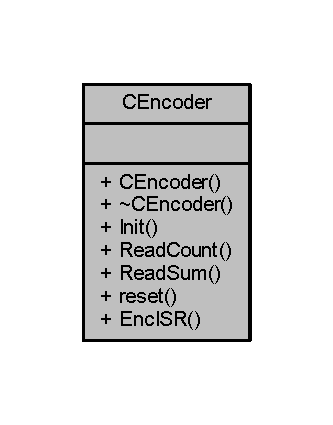
\includegraphics[width=160pt]{class_c_encoder__coll__graph}
\end{center}
\end{figure}
\subsection*{Public Types}
\begin{DoxyCompactItemize}
\item 
enum \mbox{\hyperlink{class_c_encoder_a49810cc352199fb02a60e2ef8ac6cbc3}{Encoder\+I\+D\+\_\+e}} \{ \mbox{\hyperlink{class_c_encoder_a49810cc352199fb02a60e2ef8ac6cbc3a8f0ceb6874e0c79b53bf26fa42a1b652}{E1}} = P\+I\+N\+\_\+\+E\+N\+C\+\_\+R, 
\mbox{\hyperlink{class_c_encoder_a49810cc352199fb02a60e2ef8ac6cbc3aaa314a69656e242defabd33eb8e90284}{E2}} = P\+I\+N\+\_\+\+E\+N\+C\+\_\+L
 \}
\end{DoxyCompactItemize}
\subsection*{Public Member Functions}
\begin{DoxyCompactItemize}
\item 
\mbox{\hyperlink{class_c_encoder_ab63d860ef36a6b121ab3007f70743de7}{C\+Encoder}} (\mbox{\hyperlink{class_c_encoder_a49810cc352199fb02a60e2ef8ac6cbc3}{Encoder\+I\+D\+\_\+e}} ID)
\begin{DoxyCompactList}\small\item\em Constructor of \mbox{\hyperlink{class_c_encoder}{C\+Encoder}}. \end{DoxyCompactList}\item 
\mbox{\hyperlink{class_c_encoder_aa6b7126b6e24bd115348fa6243756f47}{$\sim$\+C\+Encoder}} ()
\item 
void \mbox{\hyperlink{class_c_encoder_a99a1c676b3fd3e6f253b273b2d740aab}{Init}} ()
\begin{DoxyCompactList}\small\item\em Initialization of \mbox{\hyperlink{class_c_encoder}{C\+Encoder}}. \end{DoxyCompactList}\item 
\mbox{\hyperlink{_a_d_a_s___types_8h_a1f1825b69244eb3ad2c7165ddc99c956}{uint16\+\_\+t}} \mbox{\hyperlink{class_c_encoder_a5911a289a7ed8a32e0a89e6191e1651c}{Read\+Count}} ()
\begin{DoxyCompactList}\small\item\em Function to read out the peak count per 150ms. \end{DoxyCompactList}\item 
\mbox{\hyperlink{_a_d_a_s___types_8h_a1f1825b69244eb3ad2c7165ddc99c956}{uint16\+\_\+t}} \mbox{\hyperlink{class_c_encoder_aa38f17afea1ce9b6efd9d95335a95d26}{Read\+Sum}} ()
\begin{DoxyCompactList}\small\item\em Function to sum up the counted peaks. \end{DoxyCompactList}\item 
void \mbox{\hyperlink{class_c_encoder_ab71d6281e3f4d9f875f45368a3434980}{reset}} (void)
\begin{DoxyCompactList}\small\item\em Function to reset all values of the encoder. \end{DoxyCompactList}\item 
void \mbox{\hyperlink{class_c_encoder_aa64baac0c38ee19af8572e8da4838582}{Enc\+I\+SR}} (void)
\begin{DoxyCompactList}\small\item\em Interrupt Service Routine of the encoder. \end{DoxyCompactList}\end{DoxyCompactItemize}


\subsection{Detailed Description}


Definition at line 20 of file H\+A\+L\+\_\+\+Encoder.\+h.



\subsection{Member Enumeration Documentation}
\mbox{\Hypertarget{class_c_encoder_a49810cc352199fb02a60e2ef8ac6cbc3}\label{class_c_encoder_a49810cc352199fb02a60e2ef8ac6cbc3}} 
\index{C\+Encoder@{C\+Encoder}!Encoder\+I\+D\+\_\+e@{Encoder\+I\+D\+\_\+e}}
\index{Encoder\+I\+D\+\_\+e@{Encoder\+I\+D\+\_\+e}!C\+Encoder@{C\+Encoder}}
\subsubsection{\texorpdfstring{Encoder\+I\+D\+\_\+e}{EncoderID\_e}}
{\footnotesize\ttfamily enum \mbox{\hyperlink{class_c_encoder_a49810cc352199fb02a60e2ef8ac6cbc3}{C\+Encoder\+::\+Encoder\+I\+D\+\_\+e}}}

\begin{DoxyEnumFields}{Enumerator}
\raisebox{\heightof{T}}[0pt][0pt]{\index{E1@{E1}!C\+Encoder@{C\+Encoder}}\index{C\+Encoder@{C\+Encoder}!E1@{E1}}}\mbox{\Hypertarget{class_c_encoder_a49810cc352199fb02a60e2ef8ac6cbc3a8f0ceb6874e0c79b53bf26fa42a1b652}\label{class_c_encoder_a49810cc352199fb02a60e2ef8ac6cbc3a8f0ceb6874e0c79b53bf26fa42a1b652}} 
E1&\\
\hline

\raisebox{\heightof{T}}[0pt][0pt]{\index{E2@{E2}!C\+Encoder@{C\+Encoder}}\index{C\+Encoder@{C\+Encoder}!E2@{E2}}}\mbox{\Hypertarget{class_c_encoder_a49810cc352199fb02a60e2ef8ac6cbc3aaa314a69656e242defabd33eb8e90284}\label{class_c_encoder_a49810cc352199fb02a60e2ef8ac6cbc3aaa314a69656e242defabd33eb8e90284}} 
E2&\\
\hline

\end{DoxyEnumFields}


Definition at line 22 of file H\+A\+L\+\_\+\+Encoder.\+h.



\subsection{Constructor \& Destructor Documentation}
\mbox{\Hypertarget{class_c_encoder_ab63d860ef36a6b121ab3007f70743de7}\label{class_c_encoder_ab63d860ef36a6b121ab3007f70743de7}} 
\index{C\+Encoder@{C\+Encoder}!C\+Encoder@{C\+Encoder}}
\index{C\+Encoder@{C\+Encoder}!C\+Encoder@{C\+Encoder}}
\subsubsection{\texorpdfstring{C\+Encoder()}{CEncoder()}}
{\footnotesize\ttfamily C\+Encoder\+::\+C\+Encoder (\begin{DoxyParamCaption}\item[{\mbox{\hyperlink{class_c_encoder_a49810cc352199fb02a60e2ef8ac6cbc3}{Encoder\+I\+D\+\_\+e}}}]{ID }\end{DoxyParamCaption})}



Constructor of \mbox{\hyperlink{class_c_encoder}{C\+Encoder}}. 

Destructor of \mbox{\hyperlink{class_c_encoder}{C\+Encoder}} 

Definition at line 8 of file H\+A\+L\+\_\+\+Encoder.\+cpp.

\mbox{\Hypertarget{class_c_encoder_aa6b7126b6e24bd115348fa6243756f47}\label{class_c_encoder_aa6b7126b6e24bd115348fa6243756f47}} 
\index{C\+Encoder@{C\+Encoder}!````~C\+Encoder@{$\sim$\+C\+Encoder}}
\index{````~C\+Encoder@{$\sim$\+C\+Encoder}!C\+Encoder@{C\+Encoder}}
\subsubsection{\texorpdfstring{$\sim$\+C\+Encoder()}{~CEncoder()}}
{\footnotesize\ttfamily C\+Encoder\+::$\sim$\+C\+Encoder (\begin{DoxyParamCaption}{ }\end{DoxyParamCaption})}



Definition at line 16 of file H\+A\+L\+\_\+\+Encoder.\+cpp.



\subsection{Member Function Documentation}
\mbox{\Hypertarget{class_c_encoder_aa64baac0c38ee19af8572e8da4838582}\label{class_c_encoder_aa64baac0c38ee19af8572e8da4838582}} 
\index{C\+Encoder@{C\+Encoder}!Enc\+I\+SR@{Enc\+I\+SR}}
\index{Enc\+I\+SR@{Enc\+I\+SR}!C\+Encoder@{C\+Encoder}}
\subsubsection{\texorpdfstring{Enc\+I\+S\+R()}{EncISR()}}
{\footnotesize\ttfamily void C\+Encoder\+::\+Enc\+I\+SR (\begin{DoxyParamCaption}\item[{void}]{ }\end{DoxyParamCaption})}



Interrupt Service Routine of the encoder. 

In this I\+SR the peaks of the left encoder are counted. 

Definition at line 63 of file H\+A\+L\+\_\+\+Encoder.\+cpp.

Here is the caller graph for this function\+:
\nopagebreak
\begin{figure}[H]
\begin{center}
\leavevmode
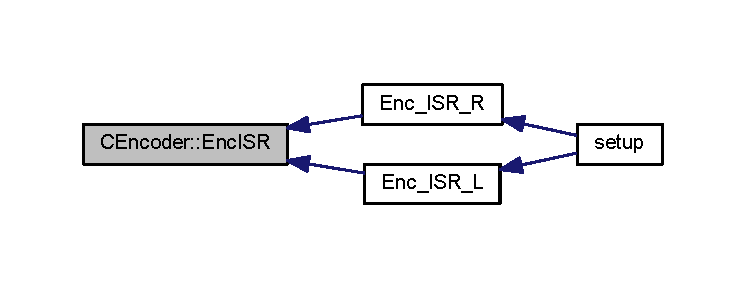
\includegraphics[width=350pt]{class_c_encoder_aa64baac0c38ee19af8572e8da4838582_icgraph}
\end{center}
\end{figure}
\mbox{\Hypertarget{class_c_encoder_a99a1c676b3fd3e6f253b273b2d740aab}\label{class_c_encoder_a99a1c676b3fd3e6f253b273b2d740aab}} 
\index{C\+Encoder@{C\+Encoder}!Init@{Init}}
\index{Init@{Init}!C\+Encoder@{C\+Encoder}}
\subsubsection{\texorpdfstring{Init()}{Init()}}
{\footnotesize\ttfamily void C\+Encoder\+::\+Init (\begin{DoxyParamCaption}\item[{void}]{ }\end{DoxyParamCaption})}



Initialization of \mbox{\hyperlink{class_c_encoder}{C\+Encoder}}. 

The pin of the encoder is initialized 

Definition at line 24 of file H\+A\+L\+\_\+\+Encoder.\+cpp.

\mbox{\Hypertarget{class_c_encoder_a5911a289a7ed8a32e0a89e6191e1651c}\label{class_c_encoder_a5911a289a7ed8a32e0a89e6191e1651c}} 
\index{C\+Encoder@{C\+Encoder}!Read\+Count@{Read\+Count}}
\index{Read\+Count@{Read\+Count}!C\+Encoder@{C\+Encoder}}
\subsubsection{\texorpdfstring{Read\+Count()}{ReadCount()}}
{\footnotesize\ttfamily \mbox{\hyperlink{_a_d_a_s___types_8h_a1f1825b69244eb3ad2c7165ddc99c956}{uint16\+\_\+t}} C\+Encoder\+::\+Read\+Count (\begin{DoxyParamCaption}{ }\end{DoxyParamCaption})}



Function to read out the peak count per 150ms. 

In this function the peaks are counted. It is called by the M\+CU every 150ms, which defines the counting time of the peaks. 

Definition at line 35 of file H\+A\+L\+\_\+\+Encoder.\+cpp.

Here is the caller graph for this function\+:
\nopagebreak
\begin{figure}[H]
\begin{center}
\leavevmode
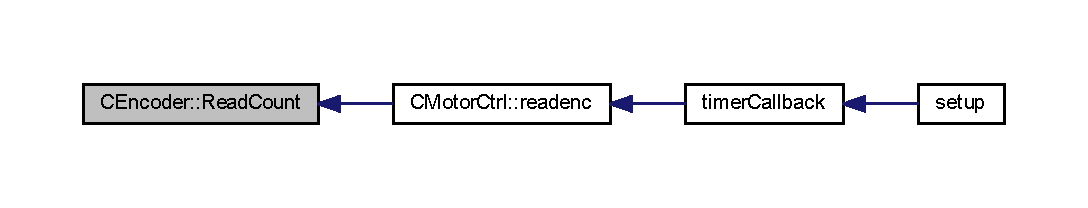
\includegraphics[width=350pt]{class_c_encoder_a5911a289a7ed8a32e0a89e6191e1651c_icgraph}
\end{center}
\end{figure}
\mbox{\Hypertarget{class_c_encoder_aa38f17afea1ce9b6efd9d95335a95d26}\label{class_c_encoder_aa38f17afea1ce9b6efd9d95335a95d26}} 
\index{C\+Encoder@{C\+Encoder}!Read\+Sum@{Read\+Sum}}
\index{Read\+Sum@{Read\+Sum}!C\+Encoder@{C\+Encoder}}
\subsubsection{\texorpdfstring{Read\+Sum()}{ReadSum()}}
{\footnotesize\ttfamily \mbox{\hyperlink{_a_d_a_s___types_8h_a1f1825b69244eb3ad2c7165ddc99c956}{uint16\+\_\+t}} C\+Encoder\+::\+Read\+Sum (\begin{DoxyParamCaption}{ }\end{DoxyParamCaption})}



Function to sum up the counted peaks. 

In this function the counted peaks per 150ms are summed up. It is called by the M\+CU every 150ms. 

Definition at line 46 of file H\+A\+L\+\_\+\+Encoder.\+cpp.

Here is the caller graph for this function\+:
\nopagebreak
\begin{figure}[H]
\begin{center}
\leavevmode
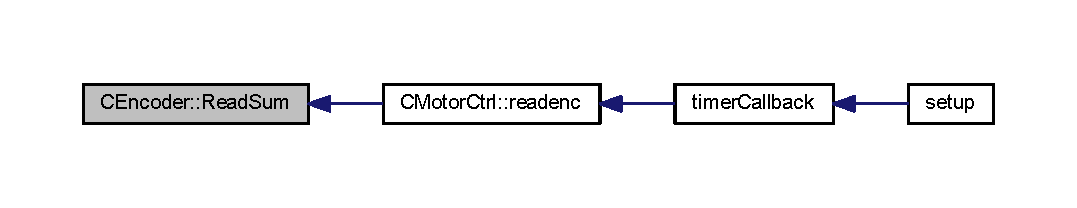
\includegraphics[width=350pt]{class_c_encoder_aa38f17afea1ce9b6efd9d95335a95d26_icgraph}
\end{center}
\end{figure}
\mbox{\Hypertarget{class_c_encoder_ab71d6281e3f4d9f875f45368a3434980}\label{class_c_encoder_ab71d6281e3f4d9f875f45368a3434980}} 
\index{C\+Encoder@{C\+Encoder}!reset@{reset}}
\index{reset@{reset}!C\+Encoder@{C\+Encoder}}
\subsubsection{\texorpdfstring{reset()}{reset()}}
{\footnotesize\ttfamily void C\+Encoder\+::reset (\begin{DoxyParamCaption}\item[{void}]{ }\end{DoxyParamCaption})}



Function to reset all values of the encoder. 



Definition at line 54 of file H\+A\+L\+\_\+\+Encoder.\+cpp.

Here is the caller graph for this function\+:
\nopagebreak
\begin{figure}[H]
\begin{center}
\leavevmode
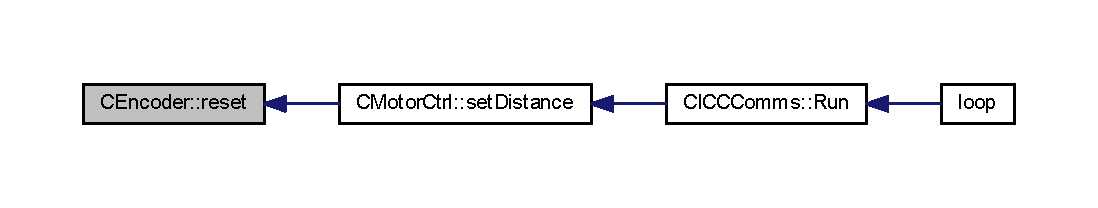
\includegraphics[width=350pt]{class_c_encoder_ab71d6281e3f4d9f875f45368a3434980_icgraph}
\end{center}
\end{figure}


The documentation for this class was generated from the following files\+:\begin{DoxyCompactItemize}
\item 
\mbox{\hyperlink{_h_a_l___encoder_8h}{H\+A\+L\+\_\+\+Encoder.\+h}}\item 
\mbox{\hyperlink{_h_a_l___encoder_8cpp}{H\+A\+L\+\_\+\+Encoder.\+cpp}}\end{DoxyCompactItemize}

\hypertarget{class_c_encoedr}{}\section{C\+Encoedr Class Reference}
\label{class_c_encoedr}\index{C\+Encoedr@{C\+Encoedr}}


Encoder Class.  




{\ttfamily \#include $<$H\+A\+L\+\_\+\+Encoder.\+h$>$}



Collaboration diagram for C\+Encoedr\+:
\nopagebreak
\begin{figure}[H]
\begin{center}
\leavevmode
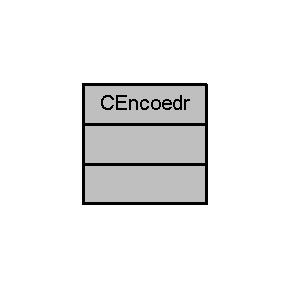
\includegraphics[width=139pt]{class_c_encoedr__coll__graph}
\end{center}
\end{figure}


\subsection{Detailed Description}
Encoder Class. 

Class declaration for the encoder 

The documentation for this class was generated from the following file\+:\begin{DoxyCompactItemize}
\item 
\mbox{\hyperlink{_h_a_l___encoder_8h}{H\+A\+L\+\_\+\+Encoder.\+h}}\end{DoxyCompactItemize}

\hypertarget{class_chart_model_class}{}\section{Chart\+Model\+Class Class Reference}
\label{class_chart_model_class}\index{ChartModelClass@{ChartModelClass}}


Class declaration of the chart model.  




{\ttfamily \#include $<$App\+\_\+\+Stateflow.\+h$>$}



Collaboration diagram for Chart\+Model\+Class\+:
% FIG 0
\subsection*{Public Member Functions}
\begin{DoxyCompactItemize}
\item 
void \mbox{\hyperlink{class_chart_model_class_ab32e055f4e5692dd69685b4befbea75d}{initialize}} ()
\begin{DoxyCompactList}\small\item\em model initialize function \end{DoxyCompactList}\item 
void \mbox{\hyperlink{class_chart_model_class_ab729e721b38bcedeed5b39c2de387413}{step}} ()
\begin{DoxyCompactList}\small\item\em model step function \end{DoxyCompactList}\item 
\mbox{\hyperlink{class_chart_model_class_ac943318da1975acdd0bee749a1372c47}{Chart\+Model\+Class}} ()
\begin{DoxyCompactList}\small\item\em Constructor. \end{DoxyCompactList}\item 
\mbox{\hyperlink{class_chart_model_class_a7b8440da4a5cbe07a6b0433db9a69f99}{$\sim$\+Chart\+Model\+Class}} ()
\begin{DoxyCompactList}\small\item\em Destructor. \end{DoxyCompactList}\item 
\mbox{\hyperlink{_app___stateflow_8h_a6f32dbbab0d15102b3fe6ec3fe6a72ba}{R\+T\+\_\+\+M\+O\+D\+EL}} $\ast$ \mbox{\hyperlink{class_chart_model_class_a77ef9eda8f1e119f93ad3c87b3a54bbd}{get\+R\+TM}} ()
\begin{DoxyCompactList}\small\item\em Real-\/\+Time Model get method. \end{DoxyCompactList}\end{DoxyCompactItemize}
\subsection*{Public Attributes}
\begin{DoxyCompactItemize}
\item 
\mbox{\hyperlink{struct_d_w}{DW}} \mbox{\hyperlink{class_chart_model_class_a1c2dcf4c77e74c040501b76bd18eebf8}{rt\+DW}}
\begin{DoxyCompactList}\small\item\em public data and function members \end{DoxyCompactList}\item 
\mbox{\hyperlink{struct_ext_u}{ExtU}} \mbox{\hyperlink{class_chart_model_class_aa557038e416c73872f813e4206084532}{rtU}}
\begin{DoxyCompactList}\small\item\em External inputs. \end{DoxyCompactList}\item 
\mbox{\hyperlink{struct_ext_y}{ExtY}} \mbox{\hyperlink{class_chart_model_class_ac7425d26c91af4aaed697e7ac65b46fa}{rtY}}
\begin{DoxyCompactList}\small\item\em External outputs. \end{DoxyCompactList}\end{DoxyCompactItemize}


\subsection{Detailed Description}
Class declaration of the chart model. 

Definition at line 110 of file App\+\_\+\+Stateflow.\+h.



\subsection{Constructor \& Destructor Documentation}
\mbox{\Hypertarget{class_chart_model_class_ac943318da1975acdd0bee749a1372c47}\label{class_chart_model_class_ac943318da1975acdd0bee749a1372c47}} 
\index{ChartModelClass@{ChartModelClass}!ChartModelClass@{ChartModelClass}}
\index{ChartModelClass@{ChartModelClass}!ChartModelClass@{ChartModelClass}}
\subsubsection{\texorpdfstring{ChartModelClass()}{ChartModelClass()}}
{\footnotesize\ttfamily Chart\+Model\+Class\+::\+Chart\+Model\+Class (\begin{DoxyParamCaption}{ }\end{DoxyParamCaption})}



Constructor. 



Definition at line 425 of file App\+\_\+\+Stateflow.\+cpp.

\mbox{\Hypertarget{class_chart_model_class_a7b8440da4a5cbe07a6b0433db9a69f99}\label{class_chart_model_class_a7b8440da4a5cbe07a6b0433db9a69f99}} 
\index{ChartModelClass@{ChartModelClass}!````~ChartModelClass@{$\sim$ChartModelClass}}
\index{````~ChartModelClass@{$\sim$ChartModelClass}!ChartModelClass@{ChartModelClass}}
\subsubsection{\texorpdfstring{$\sim$ChartModelClass()}{~ChartModelClass()}}
{\footnotesize\ttfamily Chart\+Model\+Class\+::$\sim$\+Chart\+Model\+Class (\begin{DoxyParamCaption}{ }\end{DoxyParamCaption})}



Destructor. 



Definition at line 430 of file App\+\_\+\+Stateflow.\+cpp.



\subsection{Member Function Documentation}
\mbox{\Hypertarget{class_chart_model_class_a77ef9eda8f1e119f93ad3c87b3a54bbd}\label{class_chart_model_class_a77ef9eda8f1e119f93ad3c87b3a54bbd}} 
\index{ChartModelClass@{ChartModelClass}!getRTM@{getRTM}}
\index{getRTM@{getRTM}!ChartModelClass@{ChartModelClass}}
\subsubsection{\texorpdfstring{getRTM()}{getRTM()}}
{\footnotesize\ttfamily \mbox{\hyperlink{_app___stateflow_8h_a6f32dbbab0d15102b3fe6ec3fe6a72ba}{R\+T\+\_\+\+M\+O\+D\+EL}} $\ast$ Chart\+Model\+Class\+::get\+R\+TM (\begin{DoxyParamCaption}{ }\end{DoxyParamCaption})}



Real-\/\+Time Model get method. 



Definition at line 436 of file App\+\_\+\+Stateflow.\+cpp.

Here is the caller graph for this function\+:
% FIG 1
\mbox{\Hypertarget{class_chart_model_class_ab32e055f4e5692dd69685b4befbea75d}\label{class_chart_model_class_ab32e055f4e5692dd69685b4befbea75d}} 
\index{ChartModelClass@{ChartModelClass}!initialize@{initialize}}
\index{initialize@{initialize}!ChartModelClass@{ChartModelClass}}
\subsubsection{\texorpdfstring{initialize()}{initialize()}}
{\footnotesize\ttfamily void Chart\+Model\+Class\+::initialize (\begin{DoxyParamCaption}{ }\end{DoxyParamCaption})}



model initialize function 



Definition at line 418 of file App\+\_\+\+Stateflow.\+cpp.

Here is the caller graph for this function\+:
% FIG 2
\mbox{\Hypertarget{class_chart_model_class_ab729e721b38bcedeed5b39c2de387413}\label{class_chart_model_class_ab729e721b38bcedeed5b39c2de387413}} 
\index{ChartModelClass@{ChartModelClass}!step@{step}}
\index{step@{step}!ChartModelClass@{ChartModelClass}}
\subsubsection{\texorpdfstring{step()}{step()}}
{\footnotesize\ttfamily void Chart\+Model\+Class\+::step (\begin{DoxyParamCaption}{ }\end{DoxyParamCaption})}



model step function 

Model step function. 

Definition at line 29 of file App\+\_\+\+Stateflow.\+cpp.



\subsection{Member Data Documentation}
\mbox{\Hypertarget{class_chart_model_class_a1c2dcf4c77e74c040501b76bd18eebf8}\label{class_chart_model_class_a1c2dcf4c77e74c040501b76bd18eebf8}} 
\index{ChartModelClass@{ChartModelClass}!rtDW@{rtDW}}
\index{rtDW@{rtDW}!ChartModelClass@{ChartModelClass}}
\subsubsection{\texorpdfstring{rtDW}{rtDW}}
{\footnotesize\ttfamily \mbox{\hyperlink{struct_d_w}{DW}} Chart\+Model\+Class\+::rt\+DW}



public data and function members 

Block signals and states 

Definition at line 114 of file App\+\_\+\+Stateflow.\+h.

\mbox{\Hypertarget{class_chart_model_class_aa557038e416c73872f813e4206084532}\label{class_chart_model_class_aa557038e416c73872f813e4206084532}} 
\index{ChartModelClass@{ChartModelClass}!rtU@{rtU}}
\index{rtU@{rtU}!ChartModelClass@{ChartModelClass}}
\subsubsection{\texorpdfstring{rtU}{rtU}}
{\footnotesize\ttfamily \mbox{\hyperlink{struct_ext_u}{ExtU}} Chart\+Model\+Class\+::rtU}



External inputs. 



Definition at line 116 of file App\+\_\+\+Stateflow.\+h.

\mbox{\Hypertarget{class_chart_model_class_ac7425d26c91af4aaed697e7ac65b46fa}\label{class_chart_model_class_ac7425d26c91af4aaed697e7ac65b46fa}} 
\index{ChartModelClass@{ChartModelClass}!rtY@{rtY}}
\index{rtY@{rtY}!ChartModelClass@{ChartModelClass}}
\subsubsection{\texorpdfstring{rtY}{rtY}}
{\footnotesize\ttfamily \mbox{\hyperlink{struct_ext_y}{ExtY}} Chart\+Model\+Class\+::rtY}



External outputs. 



Definition at line 119 of file App\+\_\+\+Stateflow.\+h.



The documentation for this class was generated from the following files\+:\begin{DoxyCompactItemize}
\item 
\mbox{\hyperlink{_app___stateflow_8h}{App\+\_\+\+Stateflow.\+h}}\item 
\mbox{\hyperlink{_app___stateflow_8cpp}{App\+\_\+\+Stateflow.\+cpp}}\end{DoxyCompactItemize}

\hypertarget{class_c_i_c_c_comms}{}\section{C\+I\+C\+C\+Comms Class Reference}
\label{class_c_i_c_c_comms}\index{CICCComms@{CICCComms}}


{\ttfamily \#include $<$Comm\+\_\+\+I\+C\+C.\+h$>$}



Collaboration diagram for C\+I\+C\+C\+Comms\+:
% FIG 0
\subsection*{Classes}
\begin{DoxyCompactItemize}
\item 
struct \mbox{\hyperlink{struct_c_i_c_c_comms_1_1_message__t}{Message\+\_\+t}}
\end{DoxyCompactItemize}
\subsection*{Public Member Functions}
\begin{DoxyCompactItemize}
\item 
\mbox{\hyperlink{class_c_i_c_c_comms_af2cb9bb6ab473bc5ea2b4aa2f98084ff}{C\+I\+C\+C\+Comms}} (\mbox{\hyperlink{class_c_serial}{C\+Serial}} \&ser\+Port)
\item 
\mbox{\hyperlink{class_c_i_c_c_comms_a951ae11fd2024309bd4ecf67981287e7}{$\sim$\+C\+I\+C\+C\+Comms}} ()
\item 
virtual void \mbox{\hyperlink{class_c_i_c_c_comms_a56fc0858965ed1f1f9b3295602472c7e}{Init}} (\mbox{\hyperlink{class_c_motor_ctrl}{C\+Motor\+Ctrl}} $\ast$\mbox{\hyperlink{_a_d_a_s___m_c_u_8ino_ab618fa643b3224c905b4fcbd074fb481}{m\+Ctrl\+\_\+o}})
\item 
virtual void \mbox{\hyperlink{class_c_i_c_c_comms_a8b3fa81307b3b9ba0e72b4aee8279c56}{Run}} (void)
\item 
virtual void \mbox{\hyperlink{class_c_i_c_c_comms_ab925dd7ff82f30ccd9f770ab2281b3ab}{add\+Tx\+Msg}} (\mbox{\hyperlink{_a_d_a_s___types_8h_aba7bc1797add20fe3efdf37ced1182c5}{uint8\+\_\+t}} cmd, signed int data)
\end{DoxyCompactItemize}
\subsection*{Public Attributes}
\begin{DoxyCompactItemize}
\item 
\mbox{\hyperlink{struct_c_i_c_c_comms_1_1_message__t}{Message\+\_\+t}} \mbox{\hyperlink{class_c_i_c_c_comms_a35a59d11110d830b70ab5e2a5644bbb9}{msg}}
\end{DoxyCompactItemize}


\subsection{Detailed Description}


Definition at line 17 of file Comm\+\_\+\+I\+C\+C.\+h.



\subsection{Constructor \& Destructor Documentation}
\mbox{\Hypertarget{class_c_i_c_c_comms_af2cb9bb6ab473bc5ea2b4aa2f98084ff}\label{class_c_i_c_c_comms_af2cb9bb6ab473bc5ea2b4aa2f98084ff}} 
\index{CICCComms@{CICCComms}!CICCComms@{CICCComms}}
\index{CICCComms@{CICCComms}!CICCComms@{CICCComms}}
\subsubsection{\texorpdfstring{CICCComms()}{CICCComms()}}
{\footnotesize\ttfamily C\+I\+C\+C\+Comms\+::\+C\+I\+C\+C\+Comms (\begin{DoxyParamCaption}\item[{\mbox{\hyperlink{class_c_serial}{C\+Serial}} \&}]{ser\+Port }\end{DoxyParamCaption})}



Definition at line 6 of file Comm\+\_\+\+I\+C\+C.\+cpp.

\mbox{\Hypertarget{class_c_i_c_c_comms_a951ae11fd2024309bd4ecf67981287e7}\label{class_c_i_c_c_comms_a951ae11fd2024309bd4ecf67981287e7}} 
\index{CICCComms@{CICCComms}!````~CICCComms@{$\sim$CICCComms}}
\index{````~CICCComms@{$\sim$CICCComms}!CICCComms@{CICCComms}}
\subsubsection{\texorpdfstring{$\sim$CICCComms()}{~CICCComms()}}
{\footnotesize\ttfamily C\+I\+C\+C\+Comms\+::$\sim$\+C\+I\+C\+C\+Comms (\begin{DoxyParamCaption}{ }\end{DoxyParamCaption})}



Definition at line 11 of file Comm\+\_\+\+I\+C\+C.\+cpp.



\subsection{Member Function Documentation}
\mbox{\Hypertarget{class_c_i_c_c_comms_ab925dd7ff82f30ccd9f770ab2281b3ab}\label{class_c_i_c_c_comms_ab925dd7ff82f30ccd9f770ab2281b3ab}} 
\index{CICCComms@{CICCComms}!addTxMsg@{addTxMsg}}
\index{addTxMsg@{addTxMsg}!CICCComms@{CICCComms}}
\subsubsection{\texorpdfstring{addTxMsg()}{addTxMsg()}}
{\footnotesize\ttfamily void C\+I\+C\+C\+Comms\+::add\+Tx\+Msg (\begin{DoxyParamCaption}\item[{\mbox{\hyperlink{_a_d_a_s___types_8h_aba7bc1797add20fe3efdf37ced1182c5}{uint8\+\_\+t}}}]{cmd,  }\item[{signed int}]{data }\end{DoxyParamCaption})\hspace{0.3cm}{\ttfamily [virtual]}}



Definition at line 107 of file Comm\+\_\+\+I\+C\+C.\+cpp.

\mbox{\Hypertarget{class_c_i_c_c_comms_a56fc0858965ed1f1f9b3295602472c7e}\label{class_c_i_c_c_comms_a56fc0858965ed1f1f9b3295602472c7e}} 
\index{CICCComms@{CICCComms}!Init@{Init}}
\index{Init@{Init}!CICCComms@{CICCComms}}
\subsubsection{\texorpdfstring{Init()}{Init()}}
{\footnotesize\ttfamily void C\+I\+C\+C\+Comms\+::\+Init (\begin{DoxyParamCaption}\item[{\mbox{\hyperlink{class_c_motor_ctrl}{C\+Motor\+Ctrl}} $\ast$}]{m\+Ctrl\+\_\+o }\end{DoxyParamCaption})\hspace{0.3cm}{\ttfamily [virtual]}}



Definition at line 16 of file Comm\+\_\+\+I\+C\+C.\+cpp.

Here is the caller graph for this function\+:
% FIG 1
\mbox{\Hypertarget{class_c_i_c_c_comms_a8b3fa81307b3b9ba0e72b4aee8279c56}\label{class_c_i_c_c_comms_a8b3fa81307b3b9ba0e72b4aee8279c56}} 
\index{CICCComms@{CICCComms}!Run@{Run}}
\index{Run@{Run}!CICCComms@{CICCComms}}
\subsubsection{\texorpdfstring{Run()}{Run()}}
{\footnotesize\ttfamily void C\+I\+C\+C\+Comms\+::\+Run (\begin{DoxyParamCaption}\item[{void}]{ }\end{DoxyParamCaption})\hspace{0.3cm}{\ttfamily [virtual]}}



Definition at line 21 of file Comm\+\_\+\+I\+C\+C.\+cpp.

Here is the call graph for this function\+:
% FIG 2
Here is the caller graph for this function\+:
% FIG 3


\subsection{Member Data Documentation}
\mbox{\Hypertarget{class_c_i_c_c_comms_a35a59d11110d830b70ab5e2a5644bbb9}\label{class_c_i_c_c_comms_a35a59d11110d830b70ab5e2a5644bbb9}} 
\index{CICCComms@{CICCComms}!msg@{msg}}
\index{msg@{msg}!CICCComms@{CICCComms}}
\subsubsection{\texorpdfstring{msg}{msg}}
{\footnotesize\ttfamily \mbox{\hyperlink{struct_c_i_c_c_comms_1_1_message__t}{Message\+\_\+t}} C\+I\+C\+C\+Comms\+::msg}



Definition at line 45 of file Comm\+\_\+\+I\+C\+C.\+h.



The documentation for this class was generated from the following files\+:\begin{DoxyCompactItemize}
\item 
\mbox{\hyperlink{_comm___i_c_c_8h}{Comm\+\_\+\+I\+C\+C.\+h}}\item 
\mbox{\hyperlink{_comm___i_c_c_8cpp}{Comm\+\_\+\+I\+C\+C.\+cpp}}\end{DoxyCompactItemize}

\hypertarget{class_c_i_m_u_unit}{}\section{C\+I\+M\+U\+Unit Class Reference}
\label{class_c_i_m_u_unit}\index{CIMUUnit@{CIMUUnit}}


Define class for I\+MU Unit.  




{\ttfamily \#include $<$H\+A\+L\+\_\+\+I\+M\+U.\+h$>$}



Collaboration diagram for C\+I\+M\+U\+Unit\+:
% FIG 0
\subsection*{Public Member Functions}
\begin{DoxyCompactItemize}
\item 
\mbox{\hyperlink{class_c_i_m_u_unit_a642610dac7cbec756f3ef51c5d77c344}{C\+I\+M\+U\+Unit}} ()
\begin{DoxyCompactList}\small\item\em Constructor of \mbox{\hyperlink{class_c_i_m_u_unit}{C\+I\+M\+U\+Unit}}. \end{DoxyCompactList}\item 
\mbox{\hyperlink{class_c_i_m_u_unit_ad1b0755d9d3f7f25abc660562eba6dfa}{$\sim$\+C\+I\+M\+U\+Unit}} ()
\begin{DoxyCompactList}\small\item\em Destructor of \mbox{\hyperlink{class_c_i_m_u_unit}{C\+I\+M\+U\+Unit}}. \end{DoxyCompactList}\item 
void \mbox{\hyperlink{class_c_i_m_u_unit_a589ccc2afbaadbdf9dbef34c5025a42f}{Init}} (void)
\begin{DoxyCompactList}\small\item\em Intitialization function of I\+MU Unit. \end{DoxyCompactList}\item 
\mbox{\hyperlink{_a_d_a_s___types_8h_a1f1825b69244eb3ad2c7165ddc99c956}{uint16\+\_\+t}} \mbox{\hyperlink{class_c_i_m_u_unit_a396b045fac007e169289409ca213ac39}{Return\+Gyro}} (void)
\begin{DoxyCompactList}\small\item\em Return function of I\+MU Unit Return Gyro Signal. \end{DoxyCompactList}\end{DoxyCompactItemize}


\subsection{Detailed Description}
Define class for I\+MU Unit. 

Definition at line 23 of file H\+A\+L\+\_\+\+I\+M\+U.\+h.



\subsection{Constructor \& Destructor Documentation}
\mbox{\Hypertarget{class_c_i_m_u_unit_a642610dac7cbec756f3ef51c5d77c344}\label{class_c_i_m_u_unit_a642610dac7cbec756f3ef51c5d77c344}} 
\index{CIMUUnit@{CIMUUnit}!CIMUUnit@{CIMUUnit}}
\index{CIMUUnit@{CIMUUnit}!CIMUUnit@{CIMUUnit}}
\subsubsection{\texorpdfstring{CIMUUnit()}{CIMUUnit()}}
{\footnotesize\ttfamily C\+I\+M\+U\+Unit\+::\+C\+I\+M\+U\+Unit (\begin{DoxyParamCaption}{ }\end{DoxyParamCaption})}



Constructor of \mbox{\hyperlink{class_c_i_m_u_unit}{C\+I\+M\+U\+Unit}}. 



Definition at line 22 of file H\+A\+L\+\_\+\+I\+M\+U.\+cpp.

\mbox{\Hypertarget{class_c_i_m_u_unit_ad1b0755d9d3f7f25abc660562eba6dfa}\label{class_c_i_m_u_unit_ad1b0755d9d3f7f25abc660562eba6dfa}} 
\index{CIMUUnit@{CIMUUnit}!````~CIMUUnit@{$\sim$CIMUUnit}}
\index{````~CIMUUnit@{$\sim$CIMUUnit}!CIMUUnit@{CIMUUnit}}
\subsubsection{\texorpdfstring{$\sim$CIMUUnit()}{~CIMUUnit()}}
{\footnotesize\ttfamily C\+I\+M\+U\+Unit\+::$\sim$\+C\+I\+M\+U\+Unit (\begin{DoxyParamCaption}{ }\end{DoxyParamCaption})}



Destructor of \mbox{\hyperlink{class_c_i_m_u_unit}{C\+I\+M\+U\+Unit}}. 



Definition at line 27 of file H\+A\+L\+\_\+\+I\+M\+U.\+cpp.



\subsection{Member Function Documentation}
\mbox{\Hypertarget{class_c_i_m_u_unit_a589ccc2afbaadbdf9dbef34c5025a42f}\label{class_c_i_m_u_unit_a589ccc2afbaadbdf9dbef34c5025a42f}} 
\index{CIMUUnit@{CIMUUnit}!Init@{Init}}
\index{Init@{Init}!CIMUUnit@{CIMUUnit}}
\subsubsection{\texorpdfstring{Init()}{Init()}}
{\footnotesize\ttfamily void C\+I\+M\+U\+Unit\+::\+Init (\begin{DoxyParamCaption}\item[{void}]{ }\end{DoxyParamCaption})}



Intitialization function of I\+MU Unit. 

Function checks if the sensor ready to communicate 

Definition at line 34 of file H\+A\+L\+\_\+\+I\+M\+U.\+cpp.

Here is the caller graph for this function\+:
% FIG 1
\mbox{\Hypertarget{class_c_i_m_u_unit_a396b045fac007e169289409ca213ac39}\label{class_c_i_m_u_unit_a396b045fac007e169289409ca213ac39}} 
\index{CIMUUnit@{CIMUUnit}!ReturnGyro@{ReturnGyro}}
\index{ReturnGyro@{ReturnGyro}!CIMUUnit@{CIMUUnit}}
\subsubsection{\texorpdfstring{ReturnGyro()}{ReturnGyro()}}
{\footnotesize\ttfamily \mbox{\hyperlink{_a_d_a_s___types_8h_a1f1825b69244eb3ad2c7165ddc99c956}{uint16\+\_\+t}} C\+I\+M\+U\+Unit\+::\+Return\+Gyro (\begin{DoxyParamCaption}\item[{void}]{ }\end{DoxyParamCaption})}



Return function of I\+MU Unit Return Gyro Signal. 

Function get the angles of the 3-\/axis from the gyro in degree and return the angle from x-\/axis back 

Definition at line 52 of file H\+A\+L\+\_\+\+I\+M\+U.\+cpp.

Here is the caller graph for this function\+:
% FIG 2


The documentation for this class was generated from the following files\+:\begin{DoxyCompactItemize}
\item 
\mbox{\hyperlink{_h_a_l___i_m_u_8h}{H\+A\+L\+\_\+\+I\+M\+U.\+h}}\item 
\mbox{\hyperlink{_h_a_l___i_m_u_8cpp}{H\+A\+L\+\_\+\+I\+M\+U.\+cpp}}\end{DoxyCompactItemize}

\hypertarget{class_c_inertial_comm}{}\section{C\+Inertial\+Comm Class Reference}
\label{class_c_inertial_comm}\index{CInertialComm@{CInertialComm}}


Define class for Inertial Communication.  




{\ttfamily \#include $<$Comm\+\_\+\+Inertial.\+h$>$}



Collaboration diagram for C\+Inertial\+Comm\+:
% FIG 0
\subsection*{Public Member Functions}
\begin{DoxyCompactItemize}
\item 
\mbox{\hyperlink{class_c_inertial_comm_a86917a157b0acfa80c9f178f18d882fc}{C\+Inertial\+Comm}} ()
\begin{DoxyCompactList}\small\item\em Constructor. \end{DoxyCompactList}\item 
\mbox{\hyperlink{class_c_inertial_comm_a7673549eec2f597714a39b2c4f5ab3ae}{$\sim$\+C\+Inertial\+Comm}} ()
\begin{DoxyCompactList}\small\item\em Destructor. \end{DoxyCompactList}\item 
void \mbox{\hyperlink{class_c_inertial_comm_aa8c4c1dc4ca32817bb51c520c052b4c3}{Init}} (void)
\begin{DoxyCompactList}\small\item\em Intitialization function of Inertial Communication. \end{DoxyCompactList}\item 
bool \mbox{\hyperlink{class_c_inertial_comm_ad40aa8ed083373c27fdc1aa11dfc319e}{send}} (\mbox{\hyperlink{_a_d_a_s___types_8h_aba7bc1797add20fe3efdf37ced1182c5}{uint8\+\_\+t}} buff\mbox{[}$\,$\mbox{]}, \mbox{\hyperlink{_a_d_a_s___types_8h_aba7bc1797add20fe3efdf37ced1182c5}{uint8\+\_\+t}} len)
\begin{DoxyCompactList}\small\item\em Send function of Inertial Communication. \end{DoxyCompactList}\item 
\mbox{\hyperlink{_a_d_a_s___types_8h_aba7bc1797add20fe3efdf37ced1182c5}{uint8\+\_\+t}} \mbox{\hyperlink{class_c_inertial_comm_abaed54099a0192df5a9318dc99de3668}{recieve}} (\mbox{\hyperlink{_a_d_a_s___types_8h_aba7bc1797add20fe3efdf37ced1182c5}{uint8\+\_\+t}} buff\mbox{[}$\,$\mbox{]}, \mbox{\hyperlink{_a_d_a_s___types_8h_aba7bc1797add20fe3efdf37ced1182c5}{uint8\+\_\+t}} len)
\begin{DoxyCompactList}\small\item\em Receive function of Inertial Communication. \end{DoxyCompactList}\end{DoxyCompactItemize}


\subsection{Detailed Description}
Define class for Inertial Communication. 

Definition at line 21 of file Comm\+\_\+\+Inertial.\+h.



\subsection{Constructor \& Destructor Documentation}
\mbox{\Hypertarget{class_c_inertial_comm_a86917a157b0acfa80c9f178f18d882fc}\label{class_c_inertial_comm_a86917a157b0acfa80c9f178f18d882fc}} 
\index{CInertialComm@{CInertialComm}!CInertialComm@{CInertialComm}}
\index{CInertialComm@{CInertialComm}!CInertialComm@{CInertialComm}}
\subsubsection{\texorpdfstring{CInertialComm()}{CInertialComm()}}
{\footnotesize\ttfamily C\+Inertial\+Comm\+::\+C\+Inertial\+Comm (\begin{DoxyParamCaption}{ }\end{DoxyParamCaption})}



Constructor. 

Constructor of \mbox{\hyperlink{class_c_inertial_comm}{C\+Inertial\+Comm}}. 

Definition at line 18 of file Comm\+\_\+\+Inertial.\+cpp.

\mbox{\Hypertarget{class_c_inertial_comm_a7673549eec2f597714a39b2c4f5ab3ae}\label{class_c_inertial_comm_a7673549eec2f597714a39b2c4f5ab3ae}} 
\index{CInertialComm@{CInertialComm}!````~CInertialComm@{$\sim$CInertialComm}}
\index{````~CInertialComm@{$\sim$CInertialComm}!CInertialComm@{CInertialComm}}
\subsubsection{\texorpdfstring{$\sim$CInertialComm()}{~CInertialComm()}}
{\footnotesize\ttfamily C\+Inertial\+Comm\+::$\sim$\+C\+Inertial\+Comm (\begin{DoxyParamCaption}{ }\end{DoxyParamCaption})}



Destructor. 

Destructor of \mbox{\hyperlink{class_c_inertial_comm}{C\+Inertial\+Comm}}. 

Definition at line 24 of file Comm\+\_\+\+Inertial.\+cpp.



\subsection{Member Function Documentation}
\mbox{\Hypertarget{class_c_inertial_comm_aa8c4c1dc4ca32817bb51c520c052b4c3}\label{class_c_inertial_comm_aa8c4c1dc4ca32817bb51c520c052b4c3}} 
\index{CInertialComm@{CInertialComm}!Init@{Init}}
\index{Init@{Init}!CInertialComm@{CInertialComm}}
\subsubsection{\texorpdfstring{Init()}{Init()}}
{\footnotesize\ttfamily void C\+Inertial\+Comm\+::\+Init (\begin{DoxyParamCaption}\item[{void}]{ }\end{DoxyParamCaption})}



Intitialization function of Inertial Communication. 



Definition at line 29 of file Comm\+\_\+\+Inertial.\+cpp.

\mbox{\Hypertarget{class_c_inertial_comm_abaed54099a0192df5a9318dc99de3668}\label{class_c_inertial_comm_abaed54099a0192df5a9318dc99de3668}} 
\index{CInertialComm@{CInertialComm}!recieve@{recieve}}
\index{recieve@{recieve}!CInertialComm@{CInertialComm}}
\subsubsection{\texorpdfstring{recieve()}{recieve()}}
{\footnotesize\ttfamily \mbox{\hyperlink{_a_d_a_s___types_8h_aba7bc1797add20fe3efdf37ced1182c5}{uint8\+\_\+t}} C\+Inertial\+Comm\+::recieve (\begin{DoxyParamCaption}\item[{\mbox{\hyperlink{_a_d_a_s___types_8h_aba7bc1797add20fe3efdf37ced1182c5}{uint8\+\_\+t}}}]{buff\mbox{[}$\,$\mbox{]},  }\item[{\mbox{\hyperlink{_a_d_a_s___types_8h_aba7bc1797add20fe3efdf37ced1182c5}{uint8\+\_\+t}}}]{len }\end{DoxyParamCaption})}



Receive function of Inertial Communication. 



Definition at line 40 of file Comm\+\_\+\+Inertial.\+cpp.

\mbox{\Hypertarget{class_c_inertial_comm_ad40aa8ed083373c27fdc1aa11dfc319e}\label{class_c_inertial_comm_ad40aa8ed083373c27fdc1aa11dfc319e}} 
\index{CInertialComm@{CInertialComm}!send@{send}}
\index{send@{send}!CInertialComm@{CInertialComm}}
\subsubsection{\texorpdfstring{send()}{send()}}
{\footnotesize\ttfamily bool C\+Inertial\+Comm\+::send (\begin{DoxyParamCaption}\item[{\mbox{\hyperlink{_a_d_a_s___types_8h_aba7bc1797add20fe3efdf37ced1182c5}{uint8\+\_\+t}}}]{buff\mbox{[}$\,$\mbox{]},  }\item[{\mbox{\hyperlink{_a_d_a_s___types_8h_aba7bc1797add20fe3efdf37ced1182c5}{uint8\+\_\+t}}}]{len }\end{DoxyParamCaption})}



Send function of Inertial Communication. 



Definition at line 34 of file Comm\+\_\+\+Inertial.\+cpp.



The documentation for this class was generated from the following files\+:\begin{DoxyCompactItemize}
\item 
\mbox{\hyperlink{_comm___inertial_8h}{Comm\+\_\+\+Inertial.\+h}}\item 
\mbox{\hyperlink{_comm___inertial_8cpp}{Comm\+\_\+\+Inertial.\+cpp}}\end{DoxyCompactItemize}

\hypertarget{class_c_motor_ctrl}{}\section{C\+Motor\+Ctrl Class Reference}
\label{class_c_motor_ctrl}\index{C\+Motor\+Ctrl@{C\+Motor\+Ctrl}}


Motor Control Unit Class.  




{\ttfamily \#include $<$App\+\_\+\+Motor\+Ctrl.\+h$>$}



Collaboration diagram for C\+Motor\+Ctrl\+:
\nopagebreak
\begin{figure}[H]
\begin{center}
\leavevmode
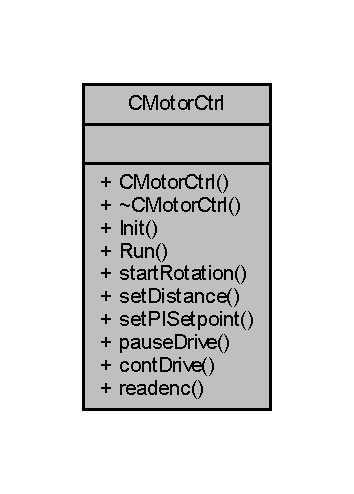
\includegraphics[width=170pt]{class_c_motor_ctrl__coll__graph}
\end{center}
\end{figure}
\subsection*{Public Member Functions}
\begin{DoxyCompactItemize}
\item 
\mbox{\hyperlink{class_c_motor_ctrl_ae51b58d3d46f718599ae4971fad86749}{C\+Motor\+Ctrl}} (\mbox{\hyperlink{class_c_i_m_u_unit}{C\+I\+M\+U\+Unit}} \&\mbox{\hyperlink{_a_d_a_s___m_c_u_8ino_ae51e36f83228f859afeb8a72e60339a6}{imu\+\_\+o}}, \mbox{\hyperlink{class_c_p_w_m_unit}{C\+P\+W\+M\+Unit}} \&\mbox{\hyperlink{_a_d_a_s___m_c_u_8ino_a10a570a59ef56c08699c4fec61d47d16}{pwm\+Unit\+Left\+\_\+o}}, \mbox{\hyperlink{class_c_p_w_m_unit}{C\+P\+W\+M\+Unit}} \&\mbox{\hyperlink{_a_d_a_s___m_c_u_8ino_a49af1ef8724d9cb785e37641bb0cdc6b}{pwm\+Unit\+Right\+\_\+o}}, \mbox{\hyperlink{class_c_encoder}{C\+Encoder}} \&\mbox{\hyperlink{_a_d_a_s___m_c_u_8ino_ad90699f8fbb0fa8f734ae5c30885ee3b}{enc1\+\_\+o}}, \mbox{\hyperlink{class_c_encoder}{C\+Encoder}} \&\mbox{\hyperlink{_a_d_a_s___m_c_u_8ino_a54cfc96aae4913b87ab356a0665557a5}{enc2\+\_\+o}}, \mbox{\hyperlink{class_c_i_c_c_comms}{C\+I\+C\+C\+Comms}} \&\mbox{\hyperlink{_a_d_a_s___m_c_u_8ino_a62ef6b3308259edb69af585549178324}{icc\+Comms\+\_\+o}})
\begin{DoxyCompactList}\small\item\em Constructor of \mbox{\hyperlink{class_c_motor_ctrl}{C\+Motor\+Ctrl}}. \end{DoxyCompactList}\item 
\mbox{\hyperlink{class_c_motor_ctrl_a97e5fbdf11c6562a7895cf4079003132}{$\sim$\+C\+Motor\+Ctrl}} ()
\begin{DoxyCompactList}\small\item\em Desctructor of \mbox{\hyperlink{class_c_motor_ctrl}{C\+Motor\+Ctrl}}. \end{DoxyCompactList}\item 
void \mbox{\hyperlink{class_c_motor_ctrl_af4b1bec8e07e766aa2537d966f025e7a}{Init}} (void)
\begin{DoxyCompactList}\small\item\em Initialization function of \mbox{\hyperlink{class_c_motor_ctrl}{C\+Motor\+Ctrl}}. \end{DoxyCompactList}\item 
void \mbox{\hyperlink{class_c_motor_ctrl_a63e5dd36be027fe8a5e1acee5c1322c8}{Run}} (void)
\begin{DoxyCompactList}\small\item\em Run function of \mbox{\hyperlink{class_c_motor_ctrl}{C\+Motor\+Ctrl}} which is executed in every loop. \end{DoxyCompactList}\item 
void \mbox{\hyperlink{class_c_motor_ctrl_a1ee991f9511437a2e64ee75161063020}{start\+Rotation}} (\mbox{\hyperlink{_a_d_a_s___types_8h_ae4c9b951dbb7355563c313abca5e2e75}{sint16\+\_\+t}} angle)
\begin{DoxyCompactList}\small\item\em A\+PI Function of the \mbox{\hyperlink{class_c_motor_ctrl}{C\+Motor\+Ctrl}} to start a rotation. \end{DoxyCompactList}\item 
void \mbox{\hyperlink{class_c_motor_ctrl_a0ae095bb6003ee63086361661f32ad3a}{set\+Distance}} (\mbox{\hyperlink{_a_d_a_s___types_8h_ae4c9b951dbb7355563c313abca5e2e75}{sint16\+\_\+t}} dist)
\begin{DoxyCompactList}\small\item\em A\+PI Function of the \mbox{\hyperlink{class_c_motor_ctrl}{C\+Motor\+Ctrl}} to start driving. \end{DoxyCompactList}\item 
void \mbox{\hyperlink{class_c_motor_ctrl_a5c6d49d9b407e46aad0abe84bcaf16ec}{set\+P\+I\+Setpoint}} (\mbox{\hyperlink{_a_d_a_s___types_8h_a1f1825b69244eb3ad2c7165ddc99c956}{uint16\+\_\+t}} setpnt)
\begin{DoxyCompactList}\small\item\em A\+PI Function of the \mbox{\hyperlink{class_c_motor_ctrl}{C\+Motor\+Ctrl}} to set a speed for the motors. \end{DoxyCompactList}\item 
void \mbox{\hyperlink{class_c_motor_ctrl_af3e047be659fb9f49f1644ba2eca4684}{pause\+Drive}} (void)
\begin{DoxyCompactList}\small\item\em A\+PI Function of the \mbox{\hyperlink{class_c_motor_ctrl}{C\+Motor\+Ctrl}} to pause the current action of the motor control. \end{DoxyCompactList}\item 
void \mbox{\hyperlink{class_c_motor_ctrl_a6b67180c355c2acf76d641f2817db66d}{cont\+Drive}} (void)
\begin{DoxyCompactList}\small\item\em A\+PI Function of the \mbox{\hyperlink{class_c_motor_ctrl}{C\+Motor\+Ctrl}} to continue the previously paused action of the motor control. \end{DoxyCompactList}\item 
void \mbox{\hyperlink{class_c_motor_ctrl_a8a76501cf8eaa85c5131bde5f33b6699}{readenc}} (void)
\begin{DoxyCompactList}\small\item\em Function of the \mbox{\hyperlink{class_c_motor_ctrl}{C\+Motor\+Ctrl}} where the sum of all peaks and the peaks per 150ms are read out. \end{DoxyCompactList}\end{DoxyCompactItemize}


\subsection{Detailed Description}
Motor Control Unit Class. 

Class declaration for motor control 

Definition at line 40 of file App\+\_\+\+Motor\+Ctrl.\+h.



\subsection{Constructor \& Destructor Documentation}
\mbox{\Hypertarget{class_c_motor_ctrl_ae51b58d3d46f718599ae4971fad86749}\label{class_c_motor_ctrl_ae51b58d3d46f718599ae4971fad86749}} 
\index{C\+Motor\+Ctrl@{C\+Motor\+Ctrl}!C\+Motor\+Ctrl@{C\+Motor\+Ctrl}}
\index{C\+Motor\+Ctrl@{C\+Motor\+Ctrl}!C\+Motor\+Ctrl@{C\+Motor\+Ctrl}}
\subsubsection{\texorpdfstring{C\+Motor\+Ctrl()}{CMotorCtrl()}}
{\footnotesize\ttfamily C\+Motor\+Ctrl\+::\+C\+Motor\+Ctrl (\begin{DoxyParamCaption}\item[{\mbox{\hyperlink{class_c_i_m_u_unit}{C\+I\+M\+U\+Unit}} \&}]{imu\+\_\+o,  }\item[{\mbox{\hyperlink{class_c_p_w_m_unit}{C\+P\+W\+M\+Unit}} \&}]{pwm\+Unit\+Left\+\_\+o,  }\item[{\mbox{\hyperlink{class_c_p_w_m_unit}{C\+P\+W\+M\+Unit}} \&}]{pwm\+Unit\+Right\+\_\+o,  }\item[{\mbox{\hyperlink{class_c_encoder}{C\+Encoder}} \&}]{enc1\+\_\+o,  }\item[{\mbox{\hyperlink{class_c_encoder}{C\+Encoder}} \&}]{enc2\+\_\+o,  }\item[{\mbox{\hyperlink{class_c_i_c_c_comms}{C\+I\+C\+C\+Comms}} \&}]{icc\+Comms\+\_\+o }\end{DoxyParamCaption})}



Constructor of \mbox{\hyperlink{class_c_motor_ctrl}{C\+Motor\+Ctrl}}. 



Definition at line 23 of file App\+\_\+\+Motor\+Ctrl.\+cpp.

\mbox{\Hypertarget{class_c_motor_ctrl_a97e5fbdf11c6562a7895cf4079003132}\label{class_c_motor_ctrl_a97e5fbdf11c6562a7895cf4079003132}} 
\index{C\+Motor\+Ctrl@{C\+Motor\+Ctrl}!````~C\+Motor\+Ctrl@{$\sim$\+C\+Motor\+Ctrl}}
\index{````~C\+Motor\+Ctrl@{$\sim$\+C\+Motor\+Ctrl}!C\+Motor\+Ctrl@{C\+Motor\+Ctrl}}
\subsubsection{\texorpdfstring{$\sim$\+C\+Motor\+Ctrl()}{~CMotorCtrl()}}
{\footnotesize\ttfamily C\+Motor\+Ctrl\+::$\sim$\+C\+Motor\+Ctrl (\begin{DoxyParamCaption}{ }\end{DoxyParamCaption})}



Desctructor of \mbox{\hyperlink{class_c_motor_ctrl}{C\+Motor\+Ctrl}}. 



Definition at line 41 of file App\+\_\+\+Motor\+Ctrl.\+cpp.



\subsection{Member Function Documentation}
\mbox{\Hypertarget{class_c_motor_ctrl_a6b67180c355c2acf76d641f2817db66d}\label{class_c_motor_ctrl_a6b67180c355c2acf76d641f2817db66d}} 
\index{C\+Motor\+Ctrl@{C\+Motor\+Ctrl}!cont\+Drive@{cont\+Drive}}
\index{cont\+Drive@{cont\+Drive}!C\+Motor\+Ctrl@{C\+Motor\+Ctrl}}
\subsubsection{\texorpdfstring{cont\+Drive()}{contDrive()}}
{\footnotesize\ttfamily void C\+Motor\+Ctrl\+::cont\+Drive (\begin{DoxyParamCaption}\item[{void}]{ }\end{DoxyParamCaption})}



A\+PI Function of the \mbox{\hyperlink{class_c_motor_ctrl}{C\+Motor\+Ctrl}} to continue the previously paused action of the motor control. 

Function sets the pause variable to false and the motor control will continue with the present action. 

Definition at line 382 of file App\+\_\+\+Motor\+Ctrl.\+cpp.

Here is the caller graph for this function\+:
\nopagebreak
\begin{figure}[H]
\begin{center}
\leavevmode
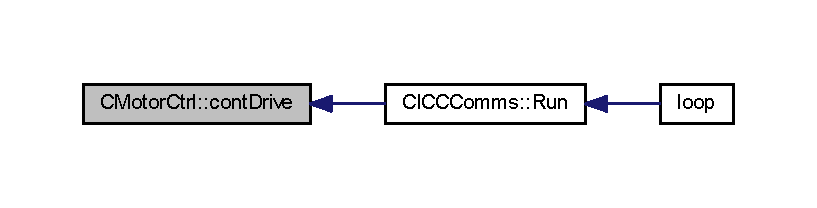
\includegraphics[width=350pt]{class_c_motor_ctrl_a6b67180c355c2acf76d641f2817db66d_icgraph}
\end{center}
\end{figure}
\mbox{\Hypertarget{class_c_motor_ctrl_af4b1bec8e07e766aa2537d966f025e7a}\label{class_c_motor_ctrl_af4b1bec8e07e766aa2537d966f025e7a}} 
\index{C\+Motor\+Ctrl@{C\+Motor\+Ctrl}!Init@{Init}}
\index{Init@{Init}!C\+Motor\+Ctrl@{C\+Motor\+Ctrl}}
\subsubsection{\texorpdfstring{Init()}{Init()}}
{\footnotesize\ttfamily void C\+Motor\+Ctrl\+::\+Init (\begin{DoxyParamCaption}\item[{void}]{ }\end{DoxyParamCaption})}



Initialization function of \mbox{\hyperlink{class_c_motor_ctrl}{C\+Motor\+Ctrl}}. 

Function set up the P\+WM signal, the I\+MU, initializes the stateflow, and initiaizes the encoder interrupts. Furthermore a timer is activated which reads out the counted peaks of the encoders every 150ms. 

Definition at line 50 of file App\+\_\+\+Motor\+Ctrl.\+cpp.

Here is the call graph for this function\+:
\nopagebreak
\begin{figure}[H]
\begin{center}
\leavevmode
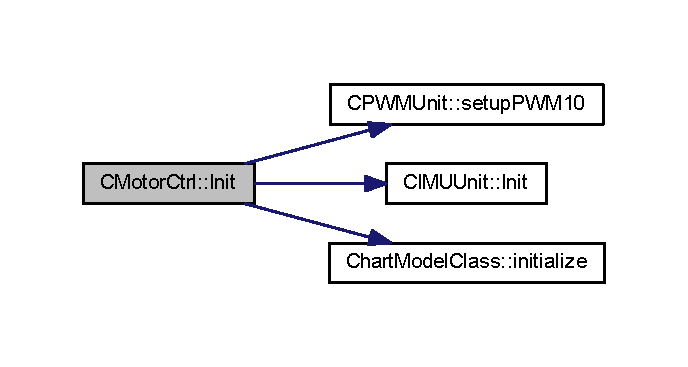
\includegraphics[width=330pt]{class_c_motor_ctrl_af4b1bec8e07e766aa2537d966f025e7a_cgraph}
\end{center}
\end{figure}
Here is the caller graph for this function\+:
\nopagebreak
\begin{figure}[H]
\begin{center}
\leavevmode
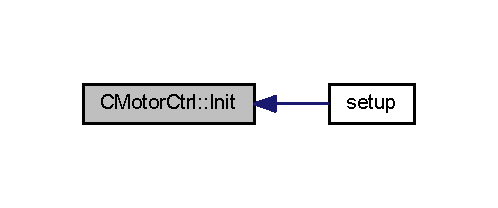
\includegraphics[width=239pt]{class_c_motor_ctrl_af4b1bec8e07e766aa2537d966f025e7a_icgraph}
\end{center}
\end{figure}
\mbox{\Hypertarget{class_c_motor_ctrl_af3e047be659fb9f49f1644ba2eca4684}\label{class_c_motor_ctrl_af3e047be659fb9f49f1644ba2eca4684}} 
\index{C\+Motor\+Ctrl@{C\+Motor\+Ctrl}!pause\+Drive@{pause\+Drive}}
\index{pause\+Drive@{pause\+Drive}!C\+Motor\+Ctrl@{C\+Motor\+Ctrl}}
\subsubsection{\texorpdfstring{pause\+Drive()}{pauseDrive()}}
{\footnotesize\ttfamily void C\+Motor\+Ctrl\+::pause\+Drive (\begin{DoxyParamCaption}\item[{void}]{ }\end{DoxyParamCaption})}



A\+PI Function of the \mbox{\hyperlink{class_c_motor_ctrl}{C\+Motor\+Ctrl}} to pause the current action of the motor control. 

Function stops the DC motors and set a pause variable to true. 

Definition at line 353 of file App\+\_\+\+Motor\+Ctrl.\+cpp.

Here is the call graph for this function\+:
\nopagebreak
\begin{figure}[H]
\begin{center}
\leavevmode
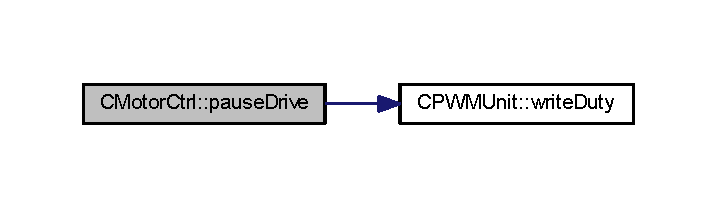
\includegraphics[width=344pt]{class_c_motor_ctrl_af3e047be659fb9f49f1644ba2eca4684_cgraph}
\end{center}
\end{figure}
Here is the caller graph for this function\+:
\nopagebreak
\begin{figure}[H]
\begin{center}
\leavevmode
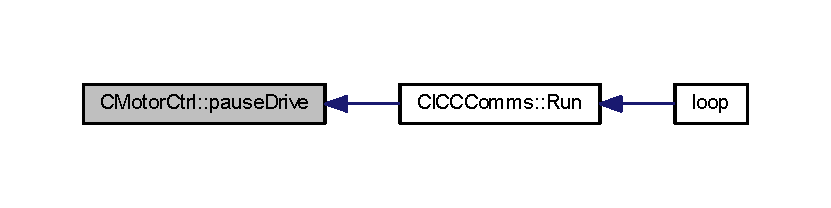
\includegraphics[width=350pt]{class_c_motor_ctrl_af3e047be659fb9f49f1644ba2eca4684_icgraph}
\end{center}
\end{figure}
\mbox{\Hypertarget{class_c_motor_ctrl_a8a76501cf8eaa85c5131bde5f33b6699}\label{class_c_motor_ctrl_a8a76501cf8eaa85c5131bde5f33b6699}} 
\index{C\+Motor\+Ctrl@{C\+Motor\+Ctrl}!readenc@{readenc}}
\index{readenc@{readenc}!C\+Motor\+Ctrl@{C\+Motor\+Ctrl}}
\subsubsection{\texorpdfstring{readenc()}{readenc()}}
{\footnotesize\ttfamily void C\+Motor\+Ctrl\+::readenc (\begin{DoxyParamCaption}\item[{void}]{ }\end{DoxyParamCaption})}



Function of the \mbox{\hyperlink{class_c_motor_ctrl}{C\+Motor\+Ctrl}} where the sum of all peaks and the peaks per 150ms are read out. 

Function is called every 150ms and reads out the count of the peaks per 150ms and sums them up. The control variable is set to true which enables the PI controller. 

Definition at line 279 of file App\+\_\+\+Motor\+Ctrl.\+cpp.

Here is the call graph for this function\+:
\nopagebreak
\begin{figure}[H]
\begin{center}
\leavevmode
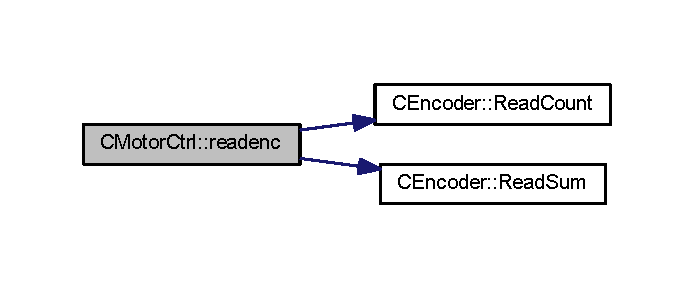
\includegraphics[width=333pt]{class_c_motor_ctrl_a8a76501cf8eaa85c5131bde5f33b6699_cgraph}
\end{center}
\end{figure}
Here is the caller graph for this function\+:
\nopagebreak
\begin{figure}[H]
\begin{center}
\leavevmode
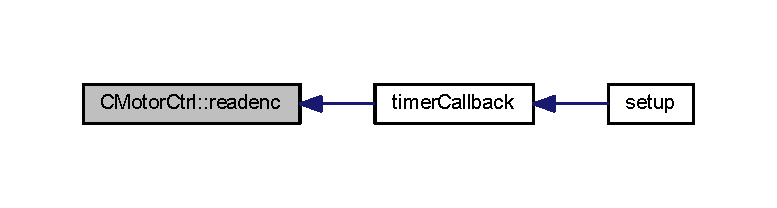
\includegraphics[width=350pt]{class_c_motor_ctrl_a8a76501cf8eaa85c5131bde5f33b6699_icgraph}
\end{center}
\end{figure}
\mbox{\Hypertarget{class_c_motor_ctrl_a63e5dd36be027fe8a5e1acee5c1322c8}\label{class_c_motor_ctrl_a63e5dd36be027fe8a5e1acee5c1322c8}} 
\index{C\+Motor\+Ctrl@{C\+Motor\+Ctrl}!Run@{Run}}
\index{Run@{Run}!C\+Motor\+Ctrl@{C\+Motor\+Ctrl}}
\subsubsection{\texorpdfstring{Run()}{Run()}}
{\footnotesize\ttfamily void C\+Motor\+Ctrl\+::\+Run (\begin{DoxyParamCaption}\item[{void}]{ }\end{DoxyParamCaption})}



Run function of \mbox{\hyperlink{class_c_motor_ctrl}{C\+Motor\+Ctrl}} which is executed in every loop. 

The function checks if the motor control stateflow is valid. If yes it is reading out the gyro sensor and performs a stateflow calculation. If the H-\/bridge is enabled and the start button was pressed it checks for the current state and runs the PI control. At the end of the function the timer for the readout function of the encoder is updated. 

Definition at line 80 of file App\+\_\+\+Motor\+Ctrl.\+cpp.

Here is the call graph for this function\+:
\nopagebreak
\begin{figure}[H]
\begin{center}
\leavevmode
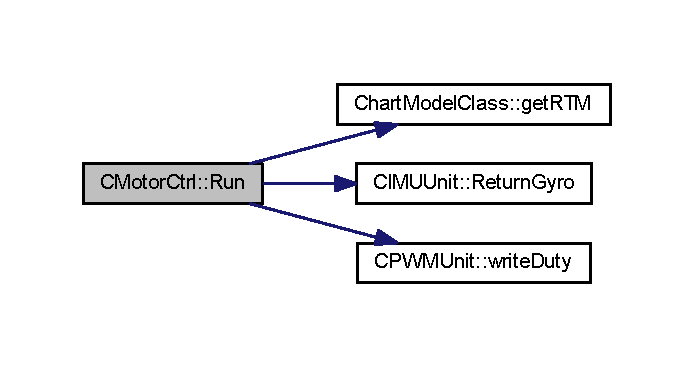
\includegraphics[width=333pt]{class_c_motor_ctrl_a63e5dd36be027fe8a5e1acee5c1322c8_cgraph}
\end{center}
\end{figure}
Here is the caller graph for this function\+:
\nopagebreak
\begin{figure}[H]
\begin{center}
\leavevmode
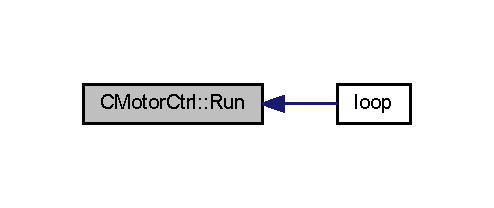
\includegraphics[width=237pt]{class_c_motor_ctrl_a63e5dd36be027fe8a5e1acee5c1322c8_icgraph}
\end{center}
\end{figure}
\mbox{\Hypertarget{class_c_motor_ctrl_a0ae095bb6003ee63086361661f32ad3a}\label{class_c_motor_ctrl_a0ae095bb6003ee63086361661f32ad3a}} 
\index{C\+Motor\+Ctrl@{C\+Motor\+Ctrl}!set\+Distance@{set\+Distance}}
\index{set\+Distance@{set\+Distance}!C\+Motor\+Ctrl@{C\+Motor\+Ctrl}}
\subsubsection{\texorpdfstring{set\+Distance()}{setDistance()}}
{\footnotesize\ttfamily void C\+Motor\+Ctrl\+::set\+Distance (\begin{DoxyParamCaption}\item[{\mbox{\hyperlink{_a_d_a_s___types_8h_ae4c9b951dbb7355563c313abca5e2e75}{sint16\+\_\+t}}}]{dist }\end{DoxyParamCaption})}



A\+PI Function of the \mbox{\hyperlink{class_c_motor_ctrl}{C\+Motor\+Ctrl}} to start driving. 

The function calculates from the transmitted distance in cm, the peaks which have to be summed up to reach the distance. The summation of all peaks are resetted and the turn variable is set to zero. Then the function checks if the distance value of the stateflow was setted previously and if the transmitted distance value is negative or positive. If the setted value is positive and the transmitted one is negative a state change from forward drive to backward drive must be performed. Same if the setted value is negative and the transmitted one is positive. 

Definition at line 309 of file App\+\_\+\+Motor\+Ctrl.\+cpp.

Here is the call graph for this function\+:
\nopagebreak
\begin{figure}[H]
\begin{center}
\leavevmode
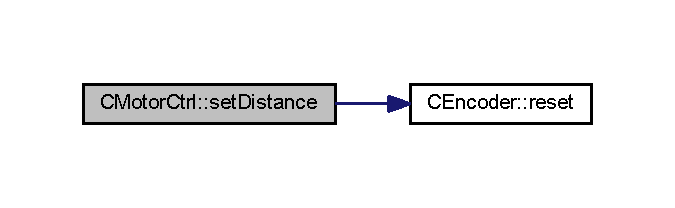
\includegraphics[width=324pt]{class_c_motor_ctrl_a0ae095bb6003ee63086361661f32ad3a_cgraph}
\end{center}
\end{figure}
Here is the caller graph for this function\+:
\nopagebreak
\begin{figure}[H]
\begin{center}
\leavevmode
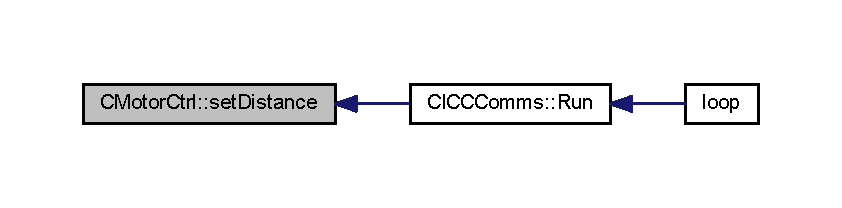
\includegraphics[width=350pt]{class_c_motor_ctrl_a0ae095bb6003ee63086361661f32ad3a_icgraph}
\end{center}
\end{figure}
\mbox{\Hypertarget{class_c_motor_ctrl_a5c6d49d9b407e46aad0abe84bcaf16ec}\label{class_c_motor_ctrl_a5c6d49d9b407e46aad0abe84bcaf16ec}} 
\index{C\+Motor\+Ctrl@{C\+Motor\+Ctrl}!set\+P\+I\+Setpoint@{set\+P\+I\+Setpoint}}
\index{set\+P\+I\+Setpoint@{set\+P\+I\+Setpoint}!C\+Motor\+Ctrl@{C\+Motor\+Ctrl}}
\subsubsection{\texorpdfstring{set\+P\+I\+Setpoint()}{setPISetpoint()}}
{\footnotesize\ttfamily void C\+Motor\+Ctrl\+::set\+P\+I\+Setpoint (\begin{DoxyParamCaption}\item[{\mbox{\hyperlink{_a_d_a_s___types_8h_a1f1825b69244eb3ad2c7165ddc99c956}{uint16\+\_\+t}}}]{setpnt }\end{DoxyParamCaption})}



A\+PI Function of the \mbox{\hyperlink{class_c_motor_ctrl}{C\+Motor\+Ctrl}} to set a speed for the motors. 

Function checks first if the desired speed is too high. If the transmitted setpoint is ok it is converted from mm/s into peaks per 150ms. Then the setpoint of the PI controllers setpoint is changed to this value. 

Definition at line 364 of file App\+\_\+\+Motor\+Ctrl.\+cpp.

\mbox{\Hypertarget{class_c_motor_ctrl_a1ee991f9511437a2e64ee75161063020}\label{class_c_motor_ctrl_a1ee991f9511437a2e64ee75161063020}} 
\index{C\+Motor\+Ctrl@{C\+Motor\+Ctrl}!start\+Rotation@{start\+Rotation}}
\index{start\+Rotation@{start\+Rotation}!C\+Motor\+Ctrl@{C\+Motor\+Ctrl}}
\subsubsection{\texorpdfstring{start\+Rotation()}{startRotation()}}
{\footnotesize\ttfamily void C\+Motor\+Ctrl\+::start\+Rotation (\begin{DoxyParamCaption}\item[{\mbox{\hyperlink{_a_d_a_s___types_8h_ae4c9b951dbb7355563c313abca5e2e75}{sint16\+\_\+t}}}]{angle }\end{DoxyParamCaption})}



A\+PI Function of the \mbox{\hyperlink{class_c_motor_ctrl}{C\+Motor\+Ctrl}} to start a rotation. 

The function sets the turn variable of the motor control stateflow to the transmitted angle and the distance to zero. A negative angle would cause a rotation to the left and a positive angle would cause a rotation to the right. 

Definition at line 295 of file App\+\_\+\+Motor\+Ctrl.\+cpp.

Here is the caller graph for this function\+:
\nopagebreak
\begin{figure}[H]
\begin{center}
\leavevmode
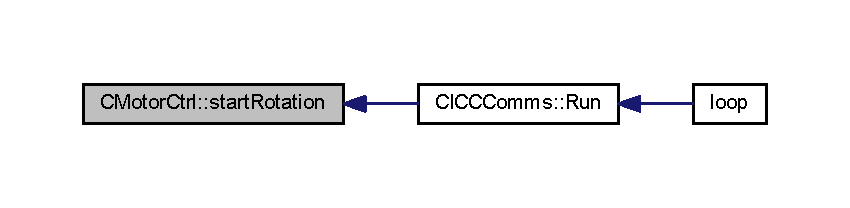
\includegraphics[width=350pt]{class_c_motor_ctrl_a1ee991f9511437a2e64ee75161063020_icgraph}
\end{center}
\end{figure}


The documentation for this class was generated from the following files\+:\begin{DoxyCompactItemize}
\item 
\mbox{\hyperlink{_app___motor_ctrl_8h}{App\+\_\+\+Motor\+Ctrl.\+h}}\item 
\mbox{\hyperlink{_app___motor_ctrl_8cpp}{App\+\_\+\+Motor\+Ctrl.\+cpp}}\end{DoxyCompactItemize}

\hypertarget{class_c_p_w_m_unit}{}\section{C\+P\+W\+M\+Unit Class Reference}
\label{class_c_p_w_m_unit}\index{C\+P\+W\+M\+Unit@{C\+P\+W\+M\+Unit}}


Hardware Abstraction Layer (H\+AL) P\+WM class.  




{\ttfamily \#include $<$H\+A\+L\+\_\+\+P\+W\+M.\+h$>$}



Collaboration diagram for C\+P\+W\+M\+Unit\+:\nopagebreak
\begin{figure}[H]
\begin{center}
\leavevmode
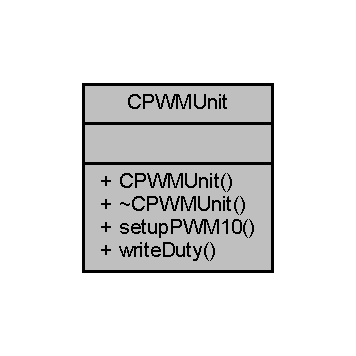
\includegraphics[width=171pt]{class_c_p_w_m_unit__coll__graph}
\end{center}
\end{figure}
\subsection*{Public Types}
\begin{DoxyCompactItemize}
\item 
enum \mbox{\hyperlink{class_c_p_w_m_unit_ad3e55d1df0367d8a090d4b835704be44}{P\+W\+M\+I\+D\+\_\+e}} \{ \mbox{\hyperlink{class_c_p_w_m_unit_ad3e55d1df0367d8a090d4b835704be44a3f6167a7882e80f1ad05c8bff5e538c0}{P\+W\+M1}} =P\+I\+N\+\_\+\+M\+T\+R\+\_\+\+L\+\_\+\+P\+WM, 
\mbox{\hyperlink{class_c_p_w_m_unit_ad3e55d1df0367d8a090d4b835704be44afc7888ea63be5da5551d10db3d676185}{P\+W\+M2}} =P\+I\+N\+\_\+\+M\+T\+R\+\_\+\+R\+\_\+\+P\+WM
 \}
\begin{DoxyCompactList}\small\item\em Enum class for P\+WM pins. \end{DoxyCompactList}\end{DoxyCompactItemize}
\subsection*{Public Member Functions}
\begin{DoxyCompactItemize}
\item 
\mbox{\hyperlink{class_c_p_w_m_unit_a9e68713e9f26f6d36714a58648494afb}{C\+P\+W\+M\+Unit}} (\mbox{\hyperlink{class_c_p_w_m_unit_ad3e55d1df0367d8a090d4b835704be44}{P\+W\+M\+I\+D\+\_\+e}} ID)
\begin{DoxyCompactList}\small\item\em Constructor of \mbox{\hyperlink{class_c_p_w_m_unit}{C\+P\+W\+M\+Unit}}. \end{DoxyCompactList}\item 
\mbox{\hyperlink{class_c_p_w_m_unit_aabfa153a1f1019befa096147428a3822}{$\sim$\+C\+P\+W\+M\+Unit}} ()
\begin{DoxyCompactList}\small\item\em Destructor of \mbox{\hyperlink{class_c_p_w_m_unit}{C\+P\+W\+M\+Unit}}. \end{DoxyCompactList}\item 
void \mbox{\hyperlink{class_c_p_w_m_unit_aa36627883e91d3dec4a76fe187588071}{setup\+P\+W\+M10}} ()
\begin{DoxyCompactList}\small\item\em Function to initialize timers for 10-\/bit P\+WM. \end{DoxyCompactList}\item 
void \mbox{\hyperlink{class_c_p_w_m_unit_a60f8be5eabf779f57e6392a0432bf7f2}{write\+Duty}} (\mbox{\hyperlink{_a_d_a_s___types_8h_a1f1825b69244eb3ad2c7165ddc99c956}{uint16\+\_\+t}} n)
\begin{DoxyCompactList}\small\item\em Function write duty cycle. \end{DoxyCompactList}\end{DoxyCompactItemize}


\subsection{Detailed Description}
Hardware Abstraction Layer (H\+AL) P\+WM class. 

Definition at line 15 of file H\+A\+L\+\_\+\+P\+W\+M.\+h.



\subsection{Member Enumeration Documentation}
\mbox{\Hypertarget{class_c_p_w_m_unit_ad3e55d1df0367d8a090d4b835704be44}\label{class_c_p_w_m_unit_ad3e55d1df0367d8a090d4b835704be44}} 
\index{C\+P\+W\+M\+Unit@{C\+P\+W\+M\+Unit}!P\+W\+M\+I\+D\+\_\+e@{P\+W\+M\+I\+D\+\_\+e}}
\index{P\+W\+M\+I\+D\+\_\+e@{P\+W\+M\+I\+D\+\_\+e}!C\+P\+W\+M\+Unit@{C\+P\+W\+M\+Unit}}
\subsubsection{\texorpdfstring{P\+W\+M\+I\+D\+\_\+e}{PWMID\_e}}
{\footnotesize\ttfamily enum \mbox{\hyperlink{class_c_p_w_m_unit_ad3e55d1df0367d8a090d4b835704be44}{C\+P\+W\+M\+Unit\+::\+P\+W\+M\+I\+D\+\_\+e}}}



Enum class for P\+WM pins. 

\begin{DoxyEnumFields}{Enumerator}
\raisebox{\heightof{T}}[0pt][0pt]{\index{P\+W\+M1@{P\+W\+M1}!C\+P\+W\+M\+Unit@{C\+P\+W\+M\+Unit}}\index{C\+P\+W\+M\+Unit@{C\+P\+W\+M\+Unit}!P\+W\+M1@{P\+W\+M1}}}\mbox{\Hypertarget{class_c_p_w_m_unit_ad3e55d1df0367d8a090d4b835704be44a3f6167a7882e80f1ad05c8bff5e538c0}\label{class_c_p_w_m_unit_ad3e55d1df0367d8a090d4b835704be44a3f6167a7882e80f1ad05c8bff5e538c0}} 
P\+W\+M1&Definition of first P\+WM pin (O\+C1A) \\
\hline

\raisebox{\heightof{T}}[0pt][0pt]{\index{P\+W\+M2@{P\+W\+M2}!C\+P\+W\+M\+Unit@{C\+P\+W\+M\+Unit}}\index{C\+P\+W\+M\+Unit@{C\+P\+W\+M\+Unit}!P\+W\+M2@{P\+W\+M2}}}\mbox{\Hypertarget{class_c_p_w_m_unit_ad3e55d1df0367d8a090d4b835704be44afc7888ea63be5da5551d10db3d676185}\label{class_c_p_w_m_unit_ad3e55d1df0367d8a090d4b835704be44afc7888ea63be5da5551d10db3d676185}} 
P\+W\+M2&Definition of second P\+WM pin (O\+C1B) \\
\hline

\end{DoxyEnumFields}


Definition at line 24 of file H\+A\+L\+\_\+\+P\+W\+M.\+h.



\subsection{Constructor \& Destructor Documentation}
\mbox{\Hypertarget{class_c_p_w_m_unit_a9e68713e9f26f6d36714a58648494afb}\label{class_c_p_w_m_unit_a9e68713e9f26f6d36714a58648494afb}} 
\index{C\+P\+W\+M\+Unit@{C\+P\+W\+M\+Unit}!C\+P\+W\+M\+Unit@{C\+P\+W\+M\+Unit}}
\index{C\+P\+W\+M\+Unit@{C\+P\+W\+M\+Unit}!C\+P\+W\+M\+Unit@{C\+P\+W\+M\+Unit}}
\subsubsection{\texorpdfstring{C\+P\+W\+M\+Unit()}{CPWMUnit()}}
{\footnotesize\ttfamily C\+P\+W\+M\+Unit\+::\+C\+P\+W\+M\+Unit (\begin{DoxyParamCaption}\item[{\mbox{\hyperlink{class_c_p_w_m_unit_ad3e55d1df0367d8a090d4b835704be44}{P\+W\+M\+I\+D\+\_\+e}}}]{ID }\end{DoxyParamCaption})}



Constructor of \mbox{\hyperlink{class_c_p_w_m_unit}{C\+P\+W\+M\+Unit}}. 

Constructor of class


\begin{DoxyParams}{Parameters}
{\em ID} & Pin number \\
\hline
\end{DoxyParams}


Definition at line 19 of file H\+A\+L\+\_\+\+P\+W\+M.\+cpp.

\mbox{\Hypertarget{class_c_p_w_m_unit_aabfa153a1f1019befa096147428a3822}\label{class_c_p_w_m_unit_aabfa153a1f1019befa096147428a3822}} 
\index{C\+P\+W\+M\+Unit@{C\+P\+W\+M\+Unit}!````~C\+P\+W\+M\+Unit@{$\sim$\+C\+P\+W\+M\+Unit}}
\index{````~C\+P\+W\+M\+Unit@{$\sim$\+C\+P\+W\+M\+Unit}!C\+P\+W\+M\+Unit@{C\+P\+W\+M\+Unit}}
\subsubsection{\texorpdfstring{$\sim$\+C\+P\+W\+M\+Unit()}{~CPWMUnit()}}
{\footnotesize\ttfamily C\+P\+W\+M\+Unit\+::$\sim$\+C\+P\+W\+M\+Unit (\begin{DoxyParamCaption}{ }\end{DoxyParamCaption})}



Destructor of \mbox{\hyperlink{class_c_p_w_m_unit}{C\+P\+W\+M\+Unit}}. 

Destructor of class 

Definition at line 25 of file H\+A\+L\+\_\+\+P\+W\+M.\+cpp.



\subsection{Member Function Documentation}
\mbox{\Hypertarget{class_c_p_w_m_unit_aa36627883e91d3dec4a76fe187588071}\label{class_c_p_w_m_unit_aa36627883e91d3dec4a76fe187588071}} 
\index{C\+P\+W\+M\+Unit@{C\+P\+W\+M\+Unit}!setup\+P\+W\+M10@{setup\+P\+W\+M10}}
\index{setup\+P\+W\+M10@{setup\+P\+W\+M10}!C\+P\+W\+M\+Unit@{C\+P\+W\+M\+Unit}}
\subsubsection{\texorpdfstring{setup\+P\+W\+M10()}{setupPWM10()}}
{\footnotesize\ttfamily void C\+P\+W\+M\+Unit\+::setup\+P\+W\+M10 (\begin{DoxyParamCaption}{ }\end{DoxyParamCaption})}



Function to initialize timers for 10-\/bit P\+WM. 



Definition at line 30 of file H\+A\+L\+\_\+\+P\+W\+M.\+cpp.

\mbox{\Hypertarget{class_c_p_w_m_unit_a60f8be5eabf779f57e6392a0432bf7f2}\label{class_c_p_w_m_unit_a60f8be5eabf779f57e6392a0432bf7f2}} 
\index{C\+P\+W\+M\+Unit@{C\+P\+W\+M\+Unit}!write\+Duty@{write\+Duty}}
\index{write\+Duty@{write\+Duty}!C\+P\+W\+M\+Unit@{C\+P\+W\+M\+Unit}}
\subsubsection{\texorpdfstring{write\+Duty()}{writeDuty()}}
{\footnotesize\ttfamily void C\+P\+W\+M\+Unit\+::write\+Duty (\begin{DoxyParamCaption}\item[{\mbox{\hyperlink{_a_d_a_s___types_8h_a1f1825b69244eb3ad2c7165ddc99c956}{uint16\+\_\+t}}}]{n }\end{DoxyParamCaption})}



Function write duty cycle. 


\begin{DoxyParams}{Parameters}
{\em n} & Duty cycle (0 = 0\% and 1023 = 100\%) \\
\hline
\end{DoxyParams}


Definition at line 63 of file H\+A\+L\+\_\+\+P\+W\+M.\+cpp.



The documentation for this class was generated from the following files\+:\begin{DoxyCompactItemize}
\item 
\mbox{\hyperlink{_h_a_l___p_w_m_8h}{H\+A\+L\+\_\+\+P\+W\+M.\+h}}\item 
\mbox{\hyperlink{_h_a_l___p_w_m_8cpp}{H\+A\+L\+\_\+\+P\+W\+M.\+cpp}}\end{DoxyCompactItemize}

\hypertarget{class_c_serial}{}\section{C\+Serial Class Reference}
\label{class_c_serial}\index{CSerial@{CSerial}}


Hardware Abstraction Layer (H\+AL) Serial class.  




{\ttfamily \#include $<$H\+A\+L\+\_\+\+Serial\+\_\+\+I\+F.\+h$>$}



Collaboration diagram for C\+Serial\+:\nopagebreak
\begin{figure}[H]
\begin{center}
\leavevmode
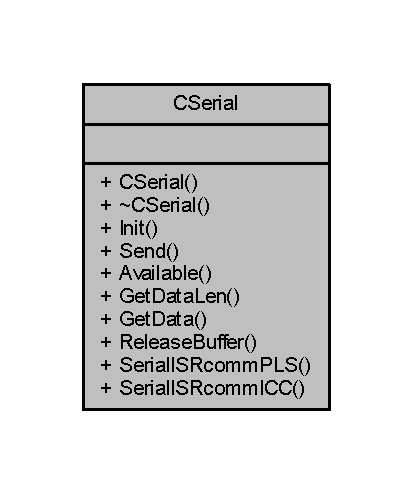
\includegraphics[width=198pt]{class_c_serial__coll__graph}
\end{center}
\end{figure}
\subsection*{Public Types}
\begin{DoxyCompactItemize}
\item 
enum \mbox{\hyperlink{class_c_serial_a000039540cc90b18bafacf5744e7eda2}{Port\+I\+D\+\_\+e}} \{ \mbox{\hyperlink{class_c_serial_a000039540cc90b18bafacf5744e7eda2a2a245d3c55e5b6e7052daf261924ce08}{S1}}, 
\mbox{\hyperlink{class_c_serial_a000039540cc90b18bafacf5744e7eda2a8cc95f4591147b0df028e003f82220a1}{S2}}
 \}
\begin{DoxyCompactList}\small\item\em Serial interface definition. \end{DoxyCompactList}\end{DoxyCompactItemize}
\subsection*{Public Member Functions}
\begin{DoxyCompactItemize}
\item 
\mbox{\hyperlink{class_c_serial_a3b2b31de1529b884b8d5e354586ee981}{C\+Serial}} (\mbox{\hyperlink{class_c_serial_a000039540cc90b18bafacf5744e7eda2}{Port\+I\+D\+\_\+e}} i\+\_\+\+ID, \mbox{\hyperlink{_a_d_a_s___types_8h_a1f1825b69244eb3ad2c7165ddc99c956}{uint16\+\_\+t}} i\+\_\+buf\+Len)
\begin{DoxyCompactList}\small\item\em Constructor of \mbox{\hyperlink{class_c_serial}{C\+Serial}}. \end{DoxyCompactList}\item 
\mbox{\hyperlink{class_c_serial_aff5444dd7e6a9ddc43cbce0e959edf7a}{$\sim$\+C\+Serial}} ()
\begin{DoxyCompactList}\small\item\em Destructor of \mbox{\hyperlink{class_c_serial}{C\+Serial}}. \end{DoxyCompactList}\item 
void \mbox{\hyperlink{class_c_serial_aed500bd204c4b37665d6d228333edafb}{Init}} (void)
\begin{DoxyCompactList}\small\item\em Initialization function of \mbox{\hyperlink{class_c_serial}{C\+Serial}}. \end{DoxyCompactList}\item 
bool \mbox{\hyperlink{class_c_serial_ae5bec6d6a1c75839ae02cf0069d1f08e}{Send}} (char Buff\mbox{[}$\,$\mbox{]}, \mbox{\hyperlink{_a_d_a_s___types_8h_aba7bc1797add20fe3efdf37ced1182c5}{uint8\+\_\+t}} len)
\begin{DoxyCompactList}\small\item\em Function to send data in transmit buffer. \end{DoxyCompactList}\item 
bool \mbox{\hyperlink{class_c_serial_abb43734223d937a86e7616636ea16024}{Available}} (void)
\begin{DoxyCompactList}\small\item\em Function to check availability of received data. \end{DoxyCompactList}\item 
\mbox{\hyperlink{_a_d_a_s___types_8h_a1f1825b69244eb3ad2c7165ddc99c956}{uint16\+\_\+t}} \mbox{\hyperlink{class_c_serial_a4327d6041fe9a390612b214709027cbb}{Get\+Data\+Len}} (void)
\begin{DoxyCompactList}\small\item\em Function to get length of data. \end{DoxyCompactList}\item 
bool \mbox{\hyperlink{class_c_serial_abad86c07f530569b2ceeea75bda485ad}{Get\+Data}} (\mbox{\hyperlink{_a_d_a_s___types_8h_aba7bc1797add20fe3efdf37ced1182c5}{uint8\+\_\+t}} $\ast$data, \mbox{\hyperlink{_a_d_a_s___types_8h_a1f1825b69244eb3ad2c7165ddc99c956}{uint16\+\_\+t}} len)
\begin{DoxyCompactList}\small\item\em Function to read data from buffer. \end{DoxyCompactList}\item 
void \mbox{\hyperlink{class_c_serial_a941e5cae2ca04518925a3b32f51110a6}{Release\+Buffer}} (void)
\begin{DoxyCompactList}\small\item\em Function to release buffer. \end{DoxyCompactList}\item 
void \mbox{\hyperlink{class_c_serial_a707841754d94fc1ab6679f52bf413d85}{Serial\+I\+S\+Rcomm\+P\+LS}} (void)
\begin{DoxyCompactList}\small\item\em Function for I\+SR U\+S\+A\+R\+Tn\+\_\+\+R\+X\+\_\+vect for P\+LS communication. \end{DoxyCompactList}\item 
void \mbox{\hyperlink{class_c_serial_a974812db5ced18cb9a6a73dc9034e7c8}{Serial\+I\+S\+Rcomm\+I\+CC}} (void)
\begin{DoxyCompactList}\small\item\em Function for I\+SR U\+S\+A\+R\+Tn\+\_\+\+R\+X\+\_\+vect for inter-\/controller communication. \end{DoxyCompactList}\end{DoxyCompactItemize}


\subsection{Detailed Description}
Hardware Abstraction Layer (H\+AL) Serial class. 

Definition at line 15 of file H\+A\+L\+\_\+\+Serial\+\_\+\+I\+F.\+h.



\subsection{Member Enumeration Documentation}
\mbox{\Hypertarget{class_c_serial_a000039540cc90b18bafacf5744e7eda2}\label{class_c_serial_a000039540cc90b18bafacf5744e7eda2}} 
\index{CSerial@{CSerial}!PortID\_e@{PortID\_e}}
\index{PortID\_e@{PortID\_e}!CSerial@{CSerial}}
\subsubsection{\texorpdfstring{PortID\_e}{PortID\_e}}
{\footnotesize\ttfamily enum \mbox{\hyperlink{class_c_serial_a000039540cc90b18bafacf5744e7eda2}{C\+Serial\+::\+Port\+I\+D\+\_\+e}}}



Serial interface definition. 

\begin{DoxyEnumFields}{Enumerator}
\raisebox{\heightof{T}}[0pt][0pt]{\index{S1@{S1}!CSerial@{CSerial}}\index{CSerial@{CSerial}!S1@{S1}}}\mbox{\Hypertarget{class_c_serial_a000039540cc90b18bafacf5744e7eda2a2a245d3c55e5b6e7052daf261924ce08}\label{class_c_serial_a000039540cc90b18bafacf5744e7eda2a2a245d3c55e5b6e7052daf261924ce08}} 
S1&Serial interface 1 \\
\hline

\raisebox{\heightof{T}}[0pt][0pt]{\index{S2@{S2}!CSerial@{CSerial}}\index{CSerial@{CSerial}!S2@{S2}}}\mbox{\Hypertarget{class_c_serial_a000039540cc90b18bafacf5744e7eda2a8cc95f4591147b0df028e003f82220a1}\label{class_c_serial_a000039540cc90b18bafacf5744e7eda2a8cc95f4591147b0df028e003f82220a1}} 
S2&Serial interface 2 \\
\hline

\end{DoxyEnumFields}


Definition at line 22 of file H\+A\+L\+\_\+\+Serial\+\_\+\+I\+F.\+h.



\subsection{Constructor \& Destructor Documentation}
\mbox{\Hypertarget{class_c_serial_a3b2b31de1529b884b8d5e354586ee981}\label{class_c_serial_a3b2b31de1529b884b8d5e354586ee981}} 
\index{CSerial@{CSerial}!CSerial@{CSerial}}
\index{CSerial@{CSerial}!CSerial@{CSerial}}
\subsubsection{\texorpdfstring{CSerial()}{CSerial()}}
{\footnotesize\ttfamily C\+Serial\+::\+C\+Serial (\begin{DoxyParamCaption}\item[{\mbox{\hyperlink{class_c_serial_a000039540cc90b18bafacf5744e7eda2}{Port\+I\+D\+\_\+e}}}]{i\+\_\+\+ID,  }\item[{\mbox{\hyperlink{_a_d_a_s___types_8h_a1f1825b69244eb3ad2c7165ddc99c956}{uint16\+\_\+t}}}]{i\+\_\+buf\+Len }\end{DoxyParamCaption})}



Constructor of \mbox{\hyperlink{class_c_serial}{C\+Serial}}. 


\begin{DoxyParams}{Parameters}
{\em i\+\_\+\+ID} & Selection of serial interace e.\+g. S1 for Serial interface 1 \\
\hline
{\em i\+\_\+buf\+Len} & Length of receiving buffer \\
\hline
\end{DoxyParams}


Definition at line 19 of file H\+A\+L\+\_\+\+Serial\+\_\+\+I\+F.\+cpp.

\mbox{\Hypertarget{class_c_serial_aff5444dd7e6a9ddc43cbce0e959edf7a}\label{class_c_serial_aff5444dd7e6a9ddc43cbce0e959edf7a}} 
\index{CSerial@{CSerial}!````~CSerial@{$\sim$CSerial}}
\index{````~CSerial@{$\sim$CSerial}!CSerial@{CSerial}}
\subsubsection{\texorpdfstring{$\sim$CSerial()}{~CSerial()}}
{\footnotesize\ttfamily C\+Serial\+::$\sim$\+C\+Serial (\begin{DoxyParamCaption}{ }\end{DoxyParamCaption})}



Destructor of \mbox{\hyperlink{class_c_serial}{C\+Serial}}. 



Definition at line 30 of file H\+A\+L\+\_\+\+Serial\+\_\+\+I\+F.\+cpp.



\subsection{Member Function Documentation}
\mbox{\Hypertarget{class_c_serial_abb43734223d937a86e7616636ea16024}\label{class_c_serial_abb43734223d937a86e7616636ea16024}} 
\index{CSerial@{CSerial}!Available@{Available}}
\index{Available@{Available}!CSerial@{CSerial}}
\subsubsection{\texorpdfstring{Available()}{Available()}}
{\footnotesize\ttfamily bool C\+Serial\+::\+Available (\begin{DoxyParamCaption}\item[{void}]{ }\end{DoxyParamCaption})}



Function to check availability of received data. 

\begin{DoxyReturn}{Returns}
Returns a true if data in buffer is available 
\end{DoxyReturn}


Definition at line 128 of file H\+A\+L\+\_\+\+Serial\+\_\+\+I\+F.\+cpp.

Here is the caller graph for this function\+:\nopagebreak
\begin{figure}[H]
\begin{center}
\leavevmode
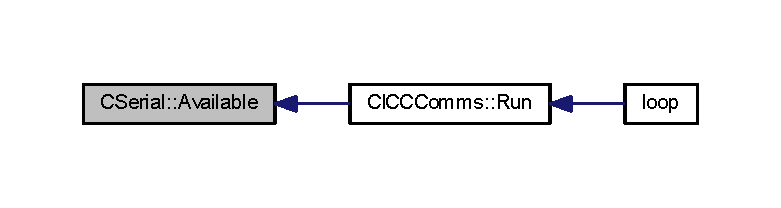
\includegraphics[width=350pt]{class_c_serial_abb43734223d937a86e7616636ea16024_icgraph}
\end{center}
\end{figure}
\mbox{\Hypertarget{class_c_serial_abad86c07f530569b2ceeea75bda485ad}\label{class_c_serial_abad86c07f530569b2ceeea75bda485ad}} 
\index{CSerial@{CSerial}!GetData@{GetData}}
\index{GetData@{GetData}!CSerial@{CSerial}}
\subsubsection{\texorpdfstring{GetData()}{GetData()}}
{\footnotesize\ttfamily bool C\+Serial\+::\+Get\+Data (\begin{DoxyParamCaption}\item[{\mbox{\hyperlink{_a_d_a_s___types_8h_aba7bc1797add20fe3efdf37ced1182c5}{uint8\+\_\+t}} $\ast$}]{data,  }\item[{\mbox{\hyperlink{_a_d_a_s___types_8h_a1f1825b69244eb3ad2c7165ddc99c956}{uint16\+\_\+t}}}]{len }\end{DoxyParamCaption})}



Function to read data from buffer. 


\begin{DoxyParams}{Parameters}
{\em data} & Pointer to destination where data shall be saved \\
\hline
{\em len} & Length of received data \\
\hline
\end{DoxyParams}
\begin{DoxyReturn}{Returns}
Returns a true of data is read 
\end{DoxyReturn}


Definition at line 148 of file H\+A\+L\+\_\+\+Serial\+\_\+\+I\+F.\+cpp.

Here is the call graph for this function\+:\nopagebreak
\begin{figure}[H]
\begin{center}
\leavevmode
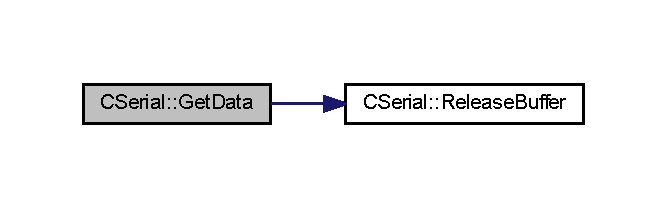
\includegraphics[width=320pt]{class_c_serial_abad86c07f530569b2ceeea75bda485ad_cgraph}
\end{center}
\end{figure}
Here is the caller graph for this function\+:\nopagebreak
\begin{figure}[H]
\begin{center}
\leavevmode
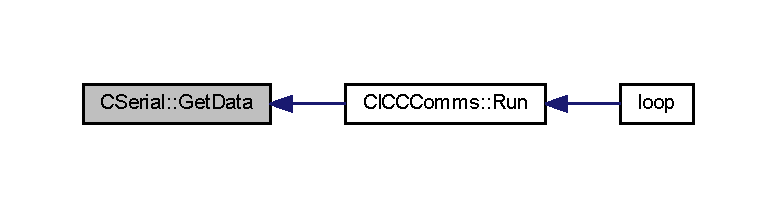
\includegraphics[width=350pt]{class_c_serial_abad86c07f530569b2ceeea75bda485ad_icgraph}
\end{center}
\end{figure}
\mbox{\Hypertarget{class_c_serial_a4327d6041fe9a390612b214709027cbb}\label{class_c_serial_a4327d6041fe9a390612b214709027cbb}} 
\index{CSerial@{CSerial}!GetDataLen@{GetDataLen}}
\index{GetDataLen@{GetDataLen}!CSerial@{CSerial}}
\subsubsection{\texorpdfstring{GetDataLen()}{GetDataLen()}}
{\footnotesize\ttfamily \mbox{\hyperlink{_a_d_a_s___types_8h_a1f1825b69244eb3ad2c7165ddc99c956}{uint16\+\_\+t}} C\+Serial\+::\+Get\+Data\+Len (\begin{DoxyParamCaption}\item[{void}]{ }\end{DoxyParamCaption})}



Function to get length of data. 

\begin{DoxyReturn}{Returns}
Returns length of data 
\end{DoxyReturn}


Definition at line 137 of file H\+A\+L\+\_\+\+Serial\+\_\+\+I\+F.\+cpp.

Here is the caller graph for this function\+:\nopagebreak
\begin{figure}[H]
\begin{center}
\leavevmode
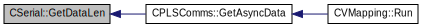
\includegraphics[width=350pt]{class_c_serial_a4327d6041fe9a390612b214709027cbb_icgraph}
\end{center}
\end{figure}
\mbox{\Hypertarget{class_c_serial_aed500bd204c4b37665d6d228333edafb}\label{class_c_serial_aed500bd204c4b37665d6d228333edafb}} 
\index{CSerial@{CSerial}!Init@{Init}}
\index{Init@{Init}!CSerial@{CSerial}}
\subsubsection{\texorpdfstring{Init()}{Init()}}
{\footnotesize\ttfamily void C\+Serial\+::\+Init (\begin{DoxyParamCaption}\item[{void}]{ }\end{DoxyParamCaption})}



Initialization function of \mbox{\hyperlink{class_c_serial}{C\+Serial}}. 



Definition at line 39 of file H\+A\+L\+\_\+\+Serial\+\_\+\+I\+F.\+cpp.

Here is the caller graph for this function\+:\nopagebreak
\begin{figure}[H]
\begin{center}
\leavevmode
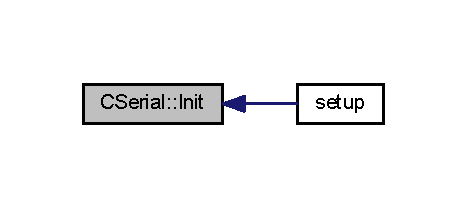
\includegraphics[width=224pt]{class_c_serial_aed500bd204c4b37665d6d228333edafb_icgraph}
\end{center}
\end{figure}
\mbox{\Hypertarget{class_c_serial_a941e5cae2ca04518925a3b32f51110a6}\label{class_c_serial_a941e5cae2ca04518925a3b32f51110a6}} 
\index{CSerial@{CSerial}!ReleaseBuffer@{ReleaseBuffer}}
\index{ReleaseBuffer@{ReleaseBuffer}!CSerial@{CSerial}}
\subsubsection{\texorpdfstring{ReleaseBuffer()}{ReleaseBuffer()}}
{\footnotesize\ttfamily void C\+Serial\+::\+Release\+Buffer (\begin{DoxyParamCaption}\item[{void}]{ }\end{DoxyParamCaption})}



Function to release buffer. 



Definition at line 161 of file H\+A\+L\+\_\+\+Serial\+\_\+\+I\+F.\+cpp.

Here is the caller graph for this function\+:\nopagebreak
\begin{figure}[H]
\begin{center}
\leavevmode
\includegraphics[width=350pt]{class_c_serial_a941e5cae2ca04518925a3b32f51110a6_icgraph}
\end{center}
\end{figure}
\mbox{\Hypertarget{class_c_serial_ae5bec6d6a1c75839ae02cf0069d1f08e}\label{class_c_serial_ae5bec6d6a1c75839ae02cf0069d1f08e}} 
\index{CSerial@{CSerial}!Send@{Send}}
\index{Send@{Send}!CSerial@{CSerial}}
\subsubsection{\texorpdfstring{Send()}{Send()}}
{\footnotesize\ttfamily bool C\+Serial\+::\+Send (\begin{DoxyParamCaption}\item[{char}]{Buff\mbox{[}$\,$\mbox{]},  }\item[{\mbox{\hyperlink{_a_d_a_s___types_8h_aba7bc1797add20fe3efdf37ced1182c5}{uint8\+\_\+t}}}]{len }\end{DoxyParamCaption})}



Function to send data in transmit buffer. 


\begin{DoxyParams}{Parameters}
{\em Buff} & Handover of transmit buffer \\
\hline
{\em len} & Length of data \\
\hline
\end{DoxyParams}
\begin{DoxyReturn}{Returns}
Returns a true if successfully sent 
\end{DoxyReturn}


Definition at line 97 of file H\+A\+L\+\_\+\+Serial\+\_\+\+I\+F.\+cpp.

\mbox{\Hypertarget{class_c_serial_a974812db5ced18cb9a6a73dc9034e7c8}\label{class_c_serial_a974812db5ced18cb9a6a73dc9034e7c8}} 
\index{CSerial@{CSerial}!SerialISRcommICC@{SerialISRcommICC}}
\index{SerialISRcommICC@{SerialISRcommICC}!CSerial@{CSerial}}
\subsubsection{\texorpdfstring{SerialISRcommICC()}{SerialISRcommICC()}}
{\footnotesize\ttfamily void C\+Serial\+::\+Serial\+I\+S\+Rcomm\+I\+CC (\begin{DoxyParamCaption}\item[{void}]{ }\end{DoxyParamCaption})}



Function for I\+SR U\+S\+A\+R\+Tn\+\_\+\+R\+X\+\_\+vect for inter-\/controller communication. 



Definition at line 215 of file H\+A\+L\+\_\+\+Serial\+\_\+\+I\+F.\+cpp.

Here is the caller graph for this function\+:
\nopagebreak
\begin{figure}[H]
\begin{center}
\leavevmode
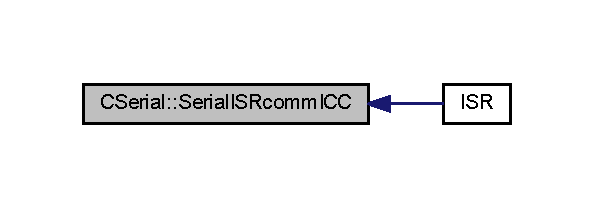
\includegraphics[width=285pt]{class_c_serial_a974812db5ced18cb9a6a73dc9034e7c8_icgraph}
\end{center}
\end{figure}
\mbox{\Hypertarget{class_c_serial_a707841754d94fc1ab6679f52bf413d85}\label{class_c_serial_a707841754d94fc1ab6679f52bf413d85}} 
\index{CSerial@{CSerial}!SerialISRcommPLS@{SerialISRcommPLS}}
\index{SerialISRcommPLS@{SerialISRcommPLS}!CSerial@{CSerial}}
\subsubsection{\texorpdfstring{SerialISRcommPLS()}{SerialISRcommPLS()}}
{\footnotesize\ttfamily void C\+Serial\+::\+Serial\+I\+S\+Rcomm\+P\+LS (\begin{DoxyParamCaption}\item[{void}]{ }\end{DoxyParamCaption})}



Function for I\+SR U\+S\+A\+R\+Tn\+\_\+\+R\+X\+\_\+vect for P\+LS communication. 



Definition at line 169 of file H\+A\+L\+\_\+\+Serial\+\_\+\+I\+F.\+cpp.

Here is the caller graph for this function\+:
\nopagebreak
\begin{figure}[H]
\begin{center}
\leavevmode
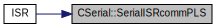
\includegraphics[width=288pt]{class_c_serial_a707841754d94fc1ab6679f52bf413d85_icgraph}
\end{center}
\end{figure}


The documentation for this class was generated from the following files\+:\begin{DoxyCompactItemize}
\item 
\mbox{\hyperlink{_h_a_l___serial___i_f_8h}{H\+A\+L\+\_\+\+Serial\+\_\+\+I\+F.\+h}}\item 
\mbox{\hyperlink{_h_a_l___serial___i_f_8cpp}{H\+A\+L\+\_\+\+Serial\+\_\+\+I\+F.\+cpp}}\end{DoxyCompactItemize}

\hypertarget{struct_d_w}{}\section{DW Struct Reference}
\label{struct_d_w}\index{DW@{DW}}


Local signals for Stateflow.  




{\ttfamily \#include $<$App\+\_\+\+Stateflow.\+h$>$}



Collaboration diagram for DW\+:
\nopagebreak
\begin{figure}[H]
\begin{center}
\leavevmode
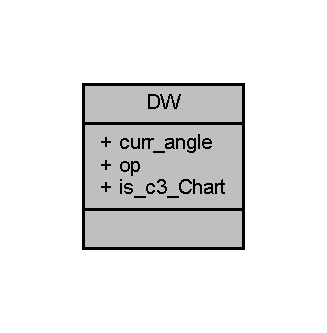
\includegraphics[width=157pt]{struct_d_w__coll__graph}
\end{center}
\end{figure}
\subsection*{Public Attributes}
\begin{DoxyCompactItemize}
\item 
\mbox{\hyperlink{_app___stateflowtypes_8h_ad73c6af88bb2ce70799e51f639309f21}{int16\+\_\+T}} \mbox{\hyperlink{struct_d_w_ab0801640ad5fc131a2c3e085d9986836}{curr\+\_\+angle}}
\begin{DoxyCompactList}\small\item\em Definition of local variable for current angle. \end{DoxyCompactList}\item 
\mbox{\hyperlink{_app___stateflowtypes_8h_ad73c6af88bb2ce70799e51f639309f21}{int16\+\_\+T}} \mbox{\hyperlink{struct_d_w_a2736d80f513d2e420f13698e8baa6c59}{op}}
\begin{DoxyCompactList}\small\item\em Definiton of local variable operation point. \end{DoxyCompactList}\item 
\mbox{\hyperlink{_app___stateflowtypes_8h_a2532a6244e023eee49f315c10f1f7c53}{uint8\+\_\+T}} \mbox{\hyperlink{struct_d_w_a3b1191ce727da1e17f5a8923eb06ae80}{is\+\_\+c3\+\_\+\+Chart}}
\begin{DoxyCompactList}\small\item\em Definiton of local variable to handle stateflow. \end{DoxyCompactList}\end{DoxyCompactItemize}


\subsection{Detailed Description}
Local signals for Stateflow. 

Definition at line 55 of file App\+\_\+\+Stateflow.\+h.



\subsection{Member Data Documentation}
\mbox{\Hypertarget{struct_d_w_ab0801640ad5fc131a2c3e085d9986836}\label{struct_d_w_ab0801640ad5fc131a2c3e085d9986836}} 
\index{DW@{DW}!curr\+\_\+angle@{curr\+\_\+angle}}
\index{curr\+\_\+angle@{curr\+\_\+angle}!DW@{DW}}
\subsubsection{\texorpdfstring{curr\+\_\+angle}{curr\_angle}}
{\footnotesize\ttfamily \mbox{\hyperlink{_app___stateflowtypes_8h_ad73c6af88bb2ce70799e51f639309f21}{int16\+\_\+T}} D\+W\+::curr\+\_\+angle}



Definition of local variable for current angle. 



Definition at line 57 of file App\+\_\+\+Stateflow.\+h.

\mbox{\Hypertarget{struct_d_w_a3b1191ce727da1e17f5a8923eb06ae80}\label{struct_d_w_a3b1191ce727da1e17f5a8923eb06ae80}} 
\index{DW@{DW}!is\+\_\+c3\+\_\+\+Chart@{is\+\_\+c3\+\_\+\+Chart}}
\index{is\+\_\+c3\+\_\+\+Chart@{is\+\_\+c3\+\_\+\+Chart}!DW@{DW}}
\subsubsection{\texorpdfstring{is\+\_\+c3\+\_\+\+Chart}{is\_c3\_Chart}}
{\footnotesize\ttfamily \mbox{\hyperlink{_app___stateflowtypes_8h_a2532a6244e023eee49f315c10f1f7c53}{uint8\+\_\+T}} D\+W\+::is\+\_\+c3\+\_\+\+Chart}



Definiton of local variable to handle stateflow. 



Definition at line 61 of file App\+\_\+\+Stateflow.\+h.

\mbox{\Hypertarget{struct_d_w_a2736d80f513d2e420f13698e8baa6c59}\label{struct_d_w_a2736d80f513d2e420f13698e8baa6c59}} 
\index{DW@{DW}!op@{op}}
\index{op@{op}!DW@{DW}}
\subsubsection{\texorpdfstring{op}{op}}
{\footnotesize\ttfamily \mbox{\hyperlink{_app___stateflowtypes_8h_ad73c6af88bb2ce70799e51f639309f21}{int16\+\_\+T}} D\+W\+::op}



Definiton of local variable operation point. 



Definition at line 59 of file App\+\_\+\+Stateflow.\+h.



The documentation for this struct was generated from the following file\+:\begin{DoxyCompactItemize}
\item 
\mbox{\hyperlink{_app___stateflow_8h}{App\+\_\+\+Stateflow.\+h}}\end{DoxyCompactItemize}

\hypertarget{struct_ext_u}{}\section{ExtU Struct Reference}
\label{struct_ext_u}\index{ExtU@{ExtU}}


External inputs for Stateflow.  




{\ttfamily \#include $<$App\+\_\+\+Stateflow.\+h$>$}



Collaboration diagram for ExtU\+:
\nopagebreak
\begin{figure}[H]
\begin{center}
\leavevmode
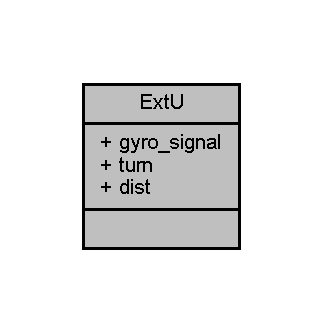
\includegraphics[width=155pt]{struct_ext_u__coll__graph}
\end{center}
\end{figure}
\subsection*{Public Attributes}
\begin{DoxyCompactItemize}
\item 
\mbox{\hyperlink{_app___stateflowtypes_8h_ad73c6af88bb2ce70799e51f639309f21}{int16\+\_\+T}} \mbox{\hyperlink{struct_ext_u_a6c0a282afef47d6b37f84bc45769e69d}{gyro\+\_\+signal}}
\begin{DoxyCompactList}\small\item\em Definition input for the gyro signal. \end{DoxyCompactList}\item 
\mbox{\hyperlink{_app___stateflowtypes_8h_ad73c6af88bb2ce70799e51f639309f21}{int16\+\_\+T}} \mbox{\hyperlink{struct_ext_u_a70e9fe496991f7c0e1fe8f54c5bf4c97}{turn}}
\begin{DoxyCompactList}\small\item\em Definition input for the turn set. \end{DoxyCompactList}\item 
\mbox{\hyperlink{_app___stateflowtypes_8h_ad73c6af88bb2ce70799e51f639309f21}{int16\+\_\+T}} \mbox{\hyperlink{struct_ext_u_a6c69fa6ebe22e9a073888b6b9dce877d}{dist}}
\begin{DoxyCompactList}\small\item\em Definition input for the distance set. \end{DoxyCompactList}\end{DoxyCompactItemize}


\subsection{Detailed Description}
External inputs for Stateflow. 

Definition at line 70 of file App\+\_\+\+Stateflow.\+h.



\subsection{Member Data Documentation}
\mbox{\Hypertarget{struct_ext_u_a6c69fa6ebe22e9a073888b6b9dce877d}\label{struct_ext_u_a6c69fa6ebe22e9a073888b6b9dce877d}} 
\index{ExtU@{ExtU}!dist@{dist}}
\index{dist@{dist}!ExtU@{ExtU}}
\subsubsection{\texorpdfstring{dist}{dist}}
{\footnotesize\ttfamily \mbox{\hyperlink{_app___stateflowtypes_8h_ad73c6af88bb2ce70799e51f639309f21}{int16\+\_\+T}} Ext\+U\+::dist}



Definition input for the distance set. 



Definition at line 76 of file App\+\_\+\+Stateflow.\+h.

\mbox{\Hypertarget{struct_ext_u_a6c0a282afef47d6b37f84bc45769e69d}\label{struct_ext_u_a6c0a282afef47d6b37f84bc45769e69d}} 
\index{ExtU@{ExtU}!gyro\+\_\+signal@{gyro\+\_\+signal}}
\index{gyro\+\_\+signal@{gyro\+\_\+signal}!ExtU@{ExtU}}
\subsubsection{\texorpdfstring{gyro\+\_\+signal}{gyro\_signal}}
{\footnotesize\ttfamily \mbox{\hyperlink{_app___stateflowtypes_8h_ad73c6af88bb2ce70799e51f639309f21}{int16\+\_\+T}} Ext\+U\+::gyro\+\_\+signal}



Definition input for the gyro signal. 



Definition at line 72 of file App\+\_\+\+Stateflow.\+h.

\mbox{\Hypertarget{struct_ext_u_a70e9fe496991f7c0e1fe8f54c5bf4c97}\label{struct_ext_u_a70e9fe496991f7c0e1fe8f54c5bf4c97}} 
\index{ExtU@{ExtU}!turn@{turn}}
\index{turn@{turn}!ExtU@{ExtU}}
\subsubsection{\texorpdfstring{turn}{turn}}
{\footnotesize\ttfamily \mbox{\hyperlink{_app___stateflowtypes_8h_ad73c6af88bb2ce70799e51f639309f21}{int16\+\_\+T}} Ext\+U\+::turn}



Definition input for the turn set. 



Definition at line 74 of file App\+\_\+\+Stateflow.\+h.



The documentation for this struct was generated from the following file\+:\begin{DoxyCompactItemize}
\item 
\mbox{\hyperlink{_app___stateflow_8h}{App\+\_\+\+Stateflow.\+h}}\end{DoxyCompactItemize}

\hypertarget{struct_ext_y}{}\section{ExtY Struct Reference}
\label{struct_ext_y}\index{ExtY@{ExtY}}


External outputs for Stateflow.  




{\ttfamily \#include $<$App\+\_\+\+Stateflow.\+h$>$}



Collaboration diagram for ExtY\+:
% FIG 0
\subsection*{Public Attributes}
\begin{DoxyCompactItemize}
\item 
\mbox{\hyperlink{_app___stateflowtypes_8h_a2532a6244e023eee49f315c10f1f7c53}{uint8\+\_\+T}} \mbox{\hyperlink{struct_ext_y_aa589c8750c337a99456c3e29975ec7fb}{mot\+\_\+r}}
\begin{DoxyCompactList}\small\item\em Definition output power motor right. \end{DoxyCompactList}\item 
\mbox{\hyperlink{_app___stateflowtypes_8h_a2532a6244e023eee49f315c10f1f7c53}{uint8\+\_\+T}} \mbox{\hyperlink{struct_ext_y_a95dca3013d0094be95ffd4af4d1a645e}{dir\+\_\+l}}
\begin{DoxyCompactList}\small\item\em Definition output direction motor left. \end{DoxyCompactList}\item 
\mbox{\hyperlink{_app___stateflowtypes_8h_a2532a6244e023eee49f315c10f1f7c53}{uint8\+\_\+T}} \mbox{\hyperlink{struct_ext_y_abe09271200dc96e32093a19312a23686}{dir\+\_\+r}}
\begin{DoxyCompactList}\small\item\em Definition output direction motor right. \end{DoxyCompactList}\item 
\mbox{\hyperlink{_app___stateflowtypes_8h_a2532a6244e023eee49f315c10f1f7c53}{uint8\+\_\+T}} \mbox{\hyperlink{struct_ext_y_a20f11c28f5b2d9f4a24766c4d56678e9}{mot\+\_\+l}}
\begin{DoxyCompactList}\small\item\em Definition output power motor right. \end{DoxyCompactList}\end{DoxyCompactItemize}


\subsection{Detailed Description}
External outputs for Stateflow. 

Definition at line 85 of file App\+\_\+\+Stateflow.\+h.



\subsection{Member Data Documentation}
\mbox{\Hypertarget{struct_ext_y_a95dca3013d0094be95ffd4af4d1a645e}\label{struct_ext_y_a95dca3013d0094be95ffd4af4d1a645e}} 
\index{ExtY@{ExtY}!dir\_l@{dir\_l}}
\index{dir\_l@{dir\_l}!ExtY@{ExtY}}
\subsubsection{\texorpdfstring{dir\_l}{dir\_l}}
{\footnotesize\ttfamily \mbox{\hyperlink{_app___stateflowtypes_8h_a2532a6244e023eee49f315c10f1f7c53}{uint8\+\_\+T}} Ext\+Y\+::dir\+\_\+l}



Definition output direction motor left. 



Definition at line 89 of file App\+\_\+\+Stateflow.\+h.

\mbox{\Hypertarget{struct_ext_y_abe09271200dc96e32093a19312a23686}\label{struct_ext_y_abe09271200dc96e32093a19312a23686}} 
\index{ExtY@{ExtY}!dir\_r@{dir\_r}}
\index{dir\_r@{dir\_r}!ExtY@{ExtY}}
\subsubsection{\texorpdfstring{dir\_r}{dir\_r}}
{\footnotesize\ttfamily \mbox{\hyperlink{_app___stateflowtypes_8h_a2532a6244e023eee49f315c10f1f7c53}{uint8\+\_\+T}} Ext\+Y\+::dir\+\_\+r}



Definition output direction motor right. 



Definition at line 91 of file App\+\_\+\+Stateflow.\+h.

\mbox{\Hypertarget{struct_ext_y_a20f11c28f5b2d9f4a24766c4d56678e9}\label{struct_ext_y_a20f11c28f5b2d9f4a24766c4d56678e9}} 
\index{ExtY@{ExtY}!mot\_l@{mot\_l}}
\index{mot\_l@{mot\_l}!ExtY@{ExtY}}
\subsubsection{\texorpdfstring{mot\_l}{mot\_l}}
{\footnotesize\ttfamily \mbox{\hyperlink{_app___stateflowtypes_8h_a2532a6244e023eee49f315c10f1f7c53}{uint8\+\_\+T}} Ext\+Y\+::mot\+\_\+l}



Definition output power motor right. 



Definition at line 93 of file App\+\_\+\+Stateflow.\+h.

\mbox{\Hypertarget{struct_ext_y_aa589c8750c337a99456c3e29975ec7fb}\label{struct_ext_y_aa589c8750c337a99456c3e29975ec7fb}} 
\index{ExtY@{ExtY}!mot\_r@{mot\_r}}
\index{mot\_r@{mot\_r}!ExtY@{ExtY}}
\subsubsection{\texorpdfstring{mot\_r}{mot\_r}}
{\footnotesize\ttfamily \mbox{\hyperlink{_app___stateflowtypes_8h_a2532a6244e023eee49f315c10f1f7c53}{uint8\+\_\+T}} Ext\+Y\+::mot\+\_\+r}



Definition output power motor right. 



Definition at line 87 of file App\+\_\+\+Stateflow.\+h.



The documentation for this struct was generated from the following file\+:\begin{DoxyCompactItemize}
\item 
\mbox{\hyperlink{_app___stateflow_8h}{App\+\_\+\+Stateflow.\+h}}\end{DoxyCompactItemize}

\hypertarget{struct_c_i_c_c_comms_1_1_message__t}{}\section{C\+I\+C\+C\+Comms\+::Message\+\_\+t Struct Reference}
\label{struct_c_i_c_c_comms_1_1_message__t}\index{CICCComms::Message\_t@{CICCComms::Message\_t}}


Structure for I\+CC messages.  




{\ttfamily \#include $<$Comm\+\_\+\+I\+C\+C.\+h$>$}



Collaboration diagram for C\+I\+C\+C\+Comms\+::Message\+\_\+t\+:
\nopagebreak
\begin{figure}[H]
\begin{center}
\leavevmode
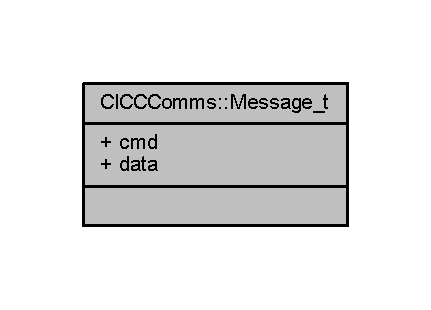
\includegraphics[width=207pt]{struct_c_i_c_c_comms_1_1_message__t__coll__graph}
\end{center}
\end{figure}
\subsection*{Public Attributes}
\begin{DoxyCompactItemize}
\item 
\mbox{\hyperlink{_a_d_a_s___types_8h_aba7bc1797add20fe3efdf37ced1182c5}{uint8\+\_\+t}} \mbox{\hyperlink{struct_c_i_c_c_comms_1_1_message__t_adf3e3290f54ee3997bc837463a340d05}{cmd}}
\item 
signed int \mbox{\hyperlink{struct_c_i_c_c_comms_1_1_message__t_a25cfce11e78d103524b695b281629d75}{data}}
\end{DoxyCompactItemize}


\subsection{Detailed Description}
Structure for I\+CC messages. 

Definition at line 26 of file Comm\+\_\+\+I\+C\+C.\+h.



\subsection{Member Data Documentation}
\mbox{\Hypertarget{struct_c_i_c_c_comms_1_1_message__t_adf3e3290f54ee3997bc837463a340d05}\label{struct_c_i_c_c_comms_1_1_message__t_adf3e3290f54ee3997bc837463a340d05}} 
\index{CICCComms::Message\_t@{CICCComms::Message\_t}!cmd@{cmd}}
\index{cmd@{cmd}!CICCComms::Message\_t@{CICCComms::Message\_t}}
\subsubsection{\texorpdfstring{cmd}{cmd}}
{\footnotesize\ttfamily \mbox{\hyperlink{_a_d_a_s___types_8h_aba7bc1797add20fe3efdf37ced1182c5}{uint8\+\_\+t}} C\+I\+C\+C\+Comms\+::\+Message\+\_\+t\+::cmd}

Command as uint8\+\_\+t 

Definition at line 27 of file Comm\+\_\+\+I\+C\+C.\+h.

\mbox{\Hypertarget{struct_c_i_c_c_comms_1_1_message__t_a25cfce11e78d103524b695b281629d75}\label{struct_c_i_c_c_comms_1_1_message__t_a25cfce11e78d103524b695b281629d75}} 
\index{CICCComms::Message\_t@{CICCComms::Message\_t}!data@{data}}
\index{data@{data}!CICCComms::Message\_t@{CICCComms::Message\_t}}
\subsubsection{\texorpdfstring{data}{data}}
{\footnotesize\ttfamily signed int C\+I\+C\+C\+Comms\+::\+Message\+\_\+t\+::data}

Data as signed int 

Definition at line 28 of file Comm\+\_\+\+I\+C\+C.\+h.



The documentation for this struct was generated from the following file\+:\begin{DoxyCompactItemize}
\item 
\mbox{\hyperlink{_comm___i_c_c_8h}{Comm\+\_\+\+I\+C\+C.\+h}}\end{DoxyCompactItemize}

\hypertarget{structtag___r_t_m}{}\section{tag\+\_\+\+R\+TM Struct Reference}
\label{structtag___r_t_m}\index{tag\_RTM@{tag\_RTM}}


Forward declaration for rt\+Model.  




{\ttfamily \#include $<$App\+\_\+\+Stateflow.\+h$>$}



Collaboration diagram for tag\+\_\+\+R\+TM\+:
% FIG 0
\subsection*{Public Attributes}
\begin{DoxyCompactItemize}
\item 
const \mbox{\hyperlink{_app___stateflowtypes_8h_a0fd897430c65dad7d2638a12bc4ea8b5}{char\+\_\+T}} $\ast$volatile \mbox{\hyperlink{structtag___r_t_m_ad977c2bc0327f9acb30208f4dc6acffe}{error\+Status}}
\end{DoxyCompactItemize}


\subsection{Detailed Description}
Forward declaration for rt\+Model. 

Real-\/time Model Data Structure for Stateflow. 

Definition at line 103 of file App\+\_\+\+Stateflow.\+h.



\subsection{Member Data Documentation}
\mbox{\Hypertarget{structtag___r_t_m_ad977c2bc0327f9acb30208f4dc6acffe}\label{structtag___r_t_m_ad977c2bc0327f9acb30208f4dc6acffe}} 
\index{tag\_RTM@{tag\_RTM}!errorStatus@{errorStatus}}
\index{errorStatus@{errorStatus}!tag\_RTM@{tag\_RTM}}
\subsubsection{\texorpdfstring{errorStatus}{errorStatus}}
{\footnotesize\ttfamily const \mbox{\hyperlink{_app___stateflowtypes_8h_a0fd897430c65dad7d2638a12bc4ea8b5}{char\+\_\+T}}$\ast$ volatile tag\+\_\+\+R\+T\+M\+::error\+Status}



Definition at line 104 of file App\+\_\+\+Stateflow.\+h.



The documentation for this struct was generated from the following file\+:\begin{DoxyCompactItemize}
\item 
\mbox{\hyperlink{_app___stateflow_8h}{App\+\_\+\+Stateflow.\+h}}\end{DoxyCompactItemize}

\chapter{File Documentation}
\hypertarget{_a_d_a_s___cfg_8h}{}\section{A\+D\+A\+S\+\_\+\+Cfg.\+h File Reference}
\label{_a_d_a_s___cfg_8h}\index{A\+D\+A\+S\+\_\+\+Cfg.\+h@{A\+D\+A\+S\+\_\+\+Cfg.\+h}}


This file contains the configuration of the vehicle.  


This graph shows which files directly or indirectly include this file\+:
\nopagebreak
\begin{figure}[H]
\begin{center}
\leavevmode
\includegraphics[width=350pt]{_a_d_a_s___cfg_8h__dep__incl}
\end{center}
\end{figure}
\subsection*{Macros}
\begin{DoxyCompactItemize}
\item 
\#define \mbox{\hyperlink{_a_d_a_s___cfg_8h_af1b7294cc1d532b3a1ab577b76852a39}{A\+D\+A\+S\+\_\+\+D\+E\+B\+U\+G2}}
\item 
\#define \mbox{\hyperlink{_a_d_a_s___cfg_8h_a00f72db64cf681b08d61977df126ec76}{P\+L\+S\+\_\+\+R\+C\+V\+\_\+\+B\+U\+F\+F\+\_\+\+S\+I\+ZE}}~500U
\item 
\#define \mbox{\hyperlink{_a_d_a_s___cfg_8h_ae3bd6bba60bc1008c82fe66f80428908}{P\+L\+S\+\_\+\+S\+N\+D\+\_\+\+B\+U\+F\+F\+\_\+\+S\+I\+ZE}}~50U
\item 
\#define \mbox{\hyperlink{_a_d_a_s___cfg_8h_abf41bed56ee0b2a8858687c4420bb110}{I\+C\+C\+\_\+\+R\+C\+V\+\_\+\+B\+U\+F\+F\+\_\+\+S\+I\+ZE}}~\mbox{\hyperlink{_a_d_a_s___cfg_8h_a17a000e80a2ce1e3be945f5484ff3dd7}{I\+C\+C\+\_\+\+L\+EN}}
\item 
\#define \mbox{\hyperlink{_a_d_a_s___cfg_8h_a5affc93ec51434d8a95645b2e3928148}{I\+C\+C\+\_\+\+S\+N\+D\+\_\+\+B\+U\+F\+F\+\_\+\+S\+I\+ZE}}~\mbox{\hyperlink{_a_d_a_s___cfg_8h_a17a000e80a2ce1e3be945f5484ff3dd7}{I\+C\+C\+\_\+\+L\+EN}}$\ast$10
\item 
\#define \mbox{\hyperlink{_a_d_a_s___cfg_8h_a4b4b233b2211ae3acf6ecf7c41f8acbb}{M\+A\+X\+\_\+\+N\+U\+M\+\_\+\+T\+A\+SK}}~5U
\item 
\#define \mbox{\hyperlink{_a_d_a_s___cfg_8h_a5ddc3cfb86290bdf3c976fc1ce56fa47}{S\+E\+R\+I\+A\+L1\+\_\+\+B\+A\+UD}}~9600
\item 
\#define \mbox{\hyperlink{_a_d_a_s___cfg_8h_ab7c4f69dae56ab78e8fb4e2c81701e77}{S\+E\+R\+I\+A\+L1\+\_\+\+B\+A\+U\+D\+\_\+\+P\+R\+E\+S\+C\+A\+LE}}~(((F\+\_\+\+C\+PU / (\mbox{\hyperlink{_a_d_a_s___cfg_8h_a5ddc3cfb86290bdf3c976fc1ce56fa47}{S\+E\+R\+I\+A\+L1\+\_\+\+B\+A\+UD}} $\ast$ 16\+U\+L))) -\/ 1)
\item 
\#define \mbox{\hyperlink{_a_d_a_s___cfg_8h_a62d0cbd008700f38d8a4fdd9aec2c554}{S\+E\+R\+I\+A\+L2\+\_\+\+B\+A\+UD}}~9600
\item 
\#define \mbox{\hyperlink{_a_d_a_s___cfg_8h_aaac720d7fe05f2b696f15ea9b2b56c7d}{S\+E\+R\+I\+A\+L2\+\_\+\+B\+A\+U\+D\+\_\+\+P\+R\+E\+S\+C\+A\+LE}}~(((F\+\_\+\+C\+PU / (\mbox{\hyperlink{_a_d_a_s___cfg_8h_a62d0cbd008700f38d8a4fdd9aec2c554}{S\+E\+R\+I\+A\+L2\+\_\+\+B\+A\+UD}} $\ast$ 16\+U\+L))) -\/ 1)
\item 
\#define \mbox{\hyperlink{_a_d_a_s___cfg_8h_aaf1f5bdadcf76f17d3f715fbbb78d567}{P\+L\+S\+\_\+\+W\+F\+\_\+\+S\+E\+G\+E\+M\+E\+N\+T\+S\+\_\+\+R\+I\+G\+HT}}~63U
\item 
\#define \mbox{\hyperlink{_a_d_a_s___cfg_8h_ad07418028b07fac4b1a3a2cc8a01a74e}{P\+L\+S\+\_\+\+W\+F\+\_\+\+S\+E\+G\+E\+M\+E\+N\+T\+S\+\_\+\+L\+E\+F\+T\+\_\+\+C\+O\+R\+N\+ER}}~117U
\item 
\#define \mbox{\hyperlink{_a_d_a_s___cfg_8h_a56c71db74384511c149652d598bf1795}{P\+L\+S\+\_\+\+W\+A\+L\+L\+\_\+\+D\+E\+T\+E\+C\+T\+I\+O\+N\+\_\+2\+\_\+\+P\+O\+I\+NT}}~45U
\item 
\#define \mbox{\hyperlink{_a_d_a_s___cfg_8h_a47e1f95a0e565aaa08112811fe539950}{P\+L\+S\+\_\+\+M\+A\+X\+\_\+\+V\+E\+R\+T\+I\+C\+A\+L\+\_\+\+D\+I\+ST}}~100U
\item 
\#define \mbox{\hyperlink{_a_d_a_s___cfg_8h_acca40b422775f8a03cd98a2e4326d906}{P\+L\+S\+\_\+\+R\+I\+G\+H\+T\+\_\+\+O\+F\+F\+S\+E\+T\+\_\+\+T\+O\+L\+E\+R\+A\+N\+CE}}~5U
\item 
\#define \mbox{\hyperlink{_a_d_a_s___cfg_8h_aedea30baea3703d1140bb971f7d1de8a}{P\+L\+S\+\_\+\+W\+F\+\_\+\+S\+E\+G\+E\+M\+E\+N\+T\+S\+\_\+\+M\+AX}}~180U
\item 
\#define \mbox{\hyperlink{_a_d_a_s___cfg_8h_a8c52736558ce47242a7c679123df76a0}{S\+I\+C\+K\+\_\+\+S\+TX}}~0x02
\item 
\#define \mbox{\hyperlink{_a_d_a_s___cfg_8h_a4ae91f90fd4b33d0bc454db3d90cf700}{S\+I\+C\+K\+\_\+\+D\+E\+S\+TR}}~0x80
\item 
\#define \mbox{\hyperlink{_a_d_a_s___cfg_8h_aa170bc1a99d2c608d5508e9b66566695}{S\+I\+C\+K\+\_\+\+A\+CK}}~0x06
\item 
\#define \mbox{\hyperlink{_a_d_a_s___cfg_8h_a6e34ca003e6bdfd81d05bcb8ea3c5eb2}{S\+I\+C\+K\+\_\+\+N\+AK}}~0x15
\item 
\#define \mbox{\hyperlink{_a_d_a_s___cfg_8h_ad9c869803f9fc9e3ffc9e962c19f028d}{P\+I\+N\+\_\+\+V\+B\+AT}}~A0
\item 
\#define \mbox{\hyperlink{_a_d_a_s___cfg_8h_a403f98f6cd7185fbd3da8bebe3406b98}{N\+A\+V\+\_\+\+S\+E\+T\+\_\+\+O\+F\+F\+S\+ET}}~80
\item 
\#define \mbox{\hyperlink{_a_d_a_s___cfg_8h_a3418793fa8fb8fe470c736d2c277e8fb}{N\+A\+V\+\_\+\+T\+O\+L\+\_\+\+O\+F\+F\+S\+ET}}~5
\item 
\#define \mbox{\hyperlink{_a_d_a_s___cfg_8h_a7ae3d3ce8d10e859369508ecb496ac07}{N\+A\+V\+\_\+\+T\+O\+L\+\_\+\+A\+N\+G\+L\+E\+\_\+\+D\+R\+I\+VE}}~5
\item 
\#define \mbox{\hyperlink{_a_d_a_s___cfg_8h_ad37cb9fe48a2b3eef8b01ec7c25d2dfc}{I\+C\+C\+\_\+\+S\+T\+X1}}~0xff
\item 
\#define \mbox{\hyperlink{_a_d_a_s___cfg_8h_a68e8b24c1a01472ef62c60e9d934f63c}{I\+C\+C\+\_\+\+S\+T\+X2}}~0xff
\item 
\#define \mbox{\hyperlink{_a_d_a_s___cfg_8h_ac9943f1124269cb02f9317d42991c503}{I\+C\+C\+\_\+\+T\+TX}}~0xee
\item 
\#define \mbox{\hyperlink{_a_d_a_s___cfg_8h_a17a000e80a2ce1e3be945f5484ff3dd7}{I\+C\+C\+\_\+\+L\+EN}}~6U
\item 
\#define \mbox{\hyperlink{_a_d_a_s___cfg_8h_a40d2abfed1ddd75059dcf6cb22827768}{I\+C\+C\+\_\+\+C\+M\+D\+\_\+\+C\+O\+N\+T\+\_\+\+D\+R\+I\+V\+E\+\_\+\+IN}}~0x01
\item 
\#define \mbox{\hyperlink{_a_d_a_s___cfg_8h_aedeacd8d3824162ab6e36fb5daf98a63}{I\+C\+C\+\_\+\+C\+M\+D\+\_\+\+E\+M\+E\+R\+\_\+\+S\+T\+OP}}~0x02
\item 
\#define \mbox{\hyperlink{_a_d_a_s___cfg_8h_a6b04b7f091aca78258644ae59974760b}{I\+C\+C\+\_\+\+C\+M\+D\+\_\+\+S\+O\+F\+T\+\_\+\+S\+T\+OP}}~0x03
\item 
\#define \mbox{\hyperlink{_a_d_a_s___cfg_8h_afdd598eb4bc8932a5361cad0bda4ce8b}{I\+C\+C\+\_\+\+C\+M\+D\+\_\+\+D\+R\+I\+V\+E\+\_\+\+D\+I\+ST}}~0x04
\item 
\#define \mbox{\hyperlink{_a_d_a_s___cfg_8h_a959554139978e2a4ac7ee923a8c0caa9}{I\+C\+C\+\_\+\+C\+M\+D\+\_\+\+R\+O\+T\+\_\+\+A\+N\+G\+LE}}~0x05
\item 
\#define \mbox{\hyperlink{_a_d_a_s___cfg_8h_aec8c3e01e4c00ebf2a58554fe92de7cd}{I\+C\+C\+\_\+\+C\+M\+D\+\_\+\+S\+E\+T\+\_\+\+S\+P\+E\+ED}}~0x06
\item 
\#define \mbox{\hyperlink{_a_d_a_s___cfg_8h_ab485c094bfdf623f14b0905c50056971}{I\+C\+C\+\_\+\+C\+M\+D\+\_\+\+P\+A\+U\+S\+E\+\_\+\+D\+R\+I\+VE}}~0x07
\item 
\#define \mbox{\hyperlink{_a_d_a_s___cfg_8h_a6ca365181dee48355653abc899f323ef}{I\+C\+C\+\_\+\+C\+M\+D\+\_\+\+C\+O\+N\+T\+\_\+\+D\+R\+I\+VE}}~0x08
\item 
\#define \mbox{\hyperlink{_a_d_a_s___cfg_8h_a9c53df5529ba6243219b7339e850b44e}{I\+C\+C\+\_\+\+C\+M\+D\+\_\+\+F\+B\+\_\+\+A\+CK}}~0x01
\item 
\#define \mbox{\hyperlink{_a_d_a_s___cfg_8h_a747531d8f8f667e12901b8cfe38c6590}{I\+C\+C\+\_\+\+C\+M\+D\+\_\+\+F\+B\+\_\+\+D\+I\+ST}}~0x02
\item 
\#define \mbox{\hyperlink{_a_d_a_s___cfg_8h_afce5749f1ae59adc2b3ac85f2a624213}{I\+C\+C\+\_\+\+C\+M\+D\+\_\+\+F\+B\+\_\+\+R\+OT}}~0x03
\item 
\#define \mbox{\hyperlink{_a_d_a_s___cfg_8h_a9b007d258cc627ea79aa06cef42c0851}{E\+N\+V\+\_\+\+V\+B\+A\+T\+\_\+\+G\+A\+IN}}~32
\item 
\#define \mbox{\hyperlink{_a_d_a_s___cfg_8h_a60f7517e6d36bf5703fc24eacb2f17ed}{E\+N\+V\+\_\+\+V\+B\+A\+T\+\_\+\+O\+FF}}~0
\item 
\#define \mbox{\hyperlink{_a_d_a_s___cfg_8h_a6975af7b117810195e5c85c0f0352474}{E\+N\+V\+\_\+\+V\+B\+A\+T\+\_\+\+L\+OW}}~22000
\item 
\#define \mbox{\hyperlink{_a_d_a_s___cfg_8h_a3b11384d6b643ae55afe2904de70a208}{E\+N\+V\+\_\+\+V\+B\+A\+T\+\_\+\+C\+RI}}~20000
\end{DoxyCompactItemize}


\subsection{Detailed Description}
This file contains the configuration of the vehicle. 

\begin{DoxyAuthor}{Author}
Christoph Jurczyk 
\end{DoxyAuthor}
\begin{DoxyDate}{Date}
January 30, 2019 
\end{DoxyDate}


\subsection{Macro Definition Documentation}
\mbox{\Hypertarget{_a_d_a_s___cfg_8h_af1b7294cc1d532b3a1ab577b76852a39}\label{_a_d_a_s___cfg_8h_af1b7294cc1d532b3a1ab577b76852a39}} 
\index{A\+D\+A\+S\+\_\+\+Cfg.\+h@{A\+D\+A\+S\+\_\+\+Cfg.\+h}!A\+D\+A\+S\+\_\+\+D\+E\+B\+U\+G2@{A\+D\+A\+S\+\_\+\+D\+E\+B\+U\+G2}}
\index{A\+D\+A\+S\+\_\+\+D\+E\+B\+U\+G2@{A\+D\+A\+S\+\_\+\+D\+E\+B\+U\+G2}!A\+D\+A\+S\+\_\+\+Cfg.\+h@{A\+D\+A\+S\+\_\+\+Cfg.\+h}}
\subsubsection{\texorpdfstring{A\+D\+A\+S\+\_\+\+D\+E\+B\+U\+G2}{ADAS\_DEBUG2}}
{\footnotesize\ttfamily \#define A\+D\+A\+S\+\_\+\+D\+E\+B\+U\+G2}

Enable this definition for debug print outs Enable this definition for debug2 print outs 

Definition at line 15 of file A\+D\+A\+S\+\_\+\+Cfg.\+h.

\mbox{\Hypertarget{_a_d_a_s___cfg_8h_a3b11384d6b643ae55afe2904de70a208}\label{_a_d_a_s___cfg_8h_a3b11384d6b643ae55afe2904de70a208}} 
\index{A\+D\+A\+S\+\_\+\+Cfg.\+h@{A\+D\+A\+S\+\_\+\+Cfg.\+h}!E\+N\+V\+\_\+\+V\+B\+A\+T\+\_\+\+C\+RI@{E\+N\+V\+\_\+\+V\+B\+A\+T\+\_\+\+C\+RI}}
\index{E\+N\+V\+\_\+\+V\+B\+A\+T\+\_\+\+C\+RI@{E\+N\+V\+\_\+\+V\+B\+A\+T\+\_\+\+C\+RI}!A\+D\+A\+S\+\_\+\+Cfg.\+h@{A\+D\+A\+S\+\_\+\+Cfg.\+h}}
\subsubsection{\texorpdfstring{E\+N\+V\+\_\+\+V\+B\+A\+T\+\_\+\+C\+RI}{ENV\_VBAT\_CRI}}
{\footnotesize\ttfamily \#define E\+N\+V\+\_\+\+V\+B\+A\+T\+\_\+\+C\+RI~20000}

Definition of critical voltage battery value 

Definition at line 119 of file A\+D\+A\+S\+\_\+\+Cfg.\+h.

\mbox{\Hypertarget{_a_d_a_s___cfg_8h_a9b007d258cc627ea79aa06cef42c0851}\label{_a_d_a_s___cfg_8h_a9b007d258cc627ea79aa06cef42c0851}} 
\index{A\+D\+A\+S\+\_\+\+Cfg.\+h@{A\+D\+A\+S\+\_\+\+Cfg.\+h}!E\+N\+V\+\_\+\+V\+B\+A\+T\+\_\+\+G\+A\+IN@{E\+N\+V\+\_\+\+V\+B\+A\+T\+\_\+\+G\+A\+IN}}
\index{E\+N\+V\+\_\+\+V\+B\+A\+T\+\_\+\+G\+A\+IN@{E\+N\+V\+\_\+\+V\+B\+A\+T\+\_\+\+G\+A\+IN}!A\+D\+A\+S\+\_\+\+Cfg.\+h@{A\+D\+A\+S\+\_\+\+Cfg.\+h}}
\subsubsection{\texorpdfstring{E\+N\+V\+\_\+\+V\+B\+A\+T\+\_\+\+G\+A\+IN}{ENV\_VBAT\_GAIN}}
{\footnotesize\ttfamily \#define E\+N\+V\+\_\+\+V\+B\+A\+T\+\_\+\+G\+A\+IN~32}

Definition of gain of the battery voltage monitor in m\+V/sample 

Definition at line 113 of file A\+D\+A\+S\+\_\+\+Cfg.\+h.

\mbox{\Hypertarget{_a_d_a_s___cfg_8h_a6975af7b117810195e5c85c0f0352474}\label{_a_d_a_s___cfg_8h_a6975af7b117810195e5c85c0f0352474}} 
\index{A\+D\+A\+S\+\_\+\+Cfg.\+h@{A\+D\+A\+S\+\_\+\+Cfg.\+h}!E\+N\+V\+\_\+\+V\+B\+A\+T\+\_\+\+L\+OW@{E\+N\+V\+\_\+\+V\+B\+A\+T\+\_\+\+L\+OW}}
\index{E\+N\+V\+\_\+\+V\+B\+A\+T\+\_\+\+L\+OW@{E\+N\+V\+\_\+\+V\+B\+A\+T\+\_\+\+L\+OW}!A\+D\+A\+S\+\_\+\+Cfg.\+h@{A\+D\+A\+S\+\_\+\+Cfg.\+h}}
\subsubsection{\texorpdfstring{E\+N\+V\+\_\+\+V\+B\+A\+T\+\_\+\+L\+OW}{ENV\_VBAT\_LOW}}
{\footnotesize\ttfamily \#define E\+N\+V\+\_\+\+V\+B\+A\+T\+\_\+\+L\+OW~22000}

Definition of low voltage battery value 

Definition at line 117 of file A\+D\+A\+S\+\_\+\+Cfg.\+h.

\mbox{\Hypertarget{_a_d_a_s___cfg_8h_a60f7517e6d36bf5703fc24eacb2f17ed}\label{_a_d_a_s___cfg_8h_a60f7517e6d36bf5703fc24eacb2f17ed}} 
\index{A\+D\+A\+S\+\_\+\+Cfg.\+h@{A\+D\+A\+S\+\_\+\+Cfg.\+h}!E\+N\+V\+\_\+\+V\+B\+A\+T\+\_\+\+O\+FF@{E\+N\+V\+\_\+\+V\+B\+A\+T\+\_\+\+O\+FF}}
\index{E\+N\+V\+\_\+\+V\+B\+A\+T\+\_\+\+O\+FF@{E\+N\+V\+\_\+\+V\+B\+A\+T\+\_\+\+O\+FF}!A\+D\+A\+S\+\_\+\+Cfg.\+h@{A\+D\+A\+S\+\_\+\+Cfg.\+h}}
\subsubsection{\texorpdfstring{E\+N\+V\+\_\+\+V\+B\+A\+T\+\_\+\+O\+FF}{ENV\_VBAT\_OFF}}
{\footnotesize\ttfamily \#define E\+N\+V\+\_\+\+V\+B\+A\+T\+\_\+\+O\+FF~0}

Definition of offset of battery voltage in mV 

Definition at line 115 of file A\+D\+A\+S\+\_\+\+Cfg.\+h.

\mbox{\Hypertarget{_a_d_a_s___cfg_8h_a6ca365181dee48355653abc899f323ef}\label{_a_d_a_s___cfg_8h_a6ca365181dee48355653abc899f323ef}} 
\index{A\+D\+A\+S\+\_\+\+Cfg.\+h@{A\+D\+A\+S\+\_\+\+Cfg.\+h}!I\+C\+C\+\_\+\+C\+M\+D\+\_\+\+C\+O\+N\+T\+\_\+\+D\+R\+I\+VE@{I\+C\+C\+\_\+\+C\+M\+D\+\_\+\+C\+O\+N\+T\+\_\+\+D\+R\+I\+VE}}
\index{I\+C\+C\+\_\+\+C\+M\+D\+\_\+\+C\+O\+N\+T\+\_\+\+D\+R\+I\+VE@{I\+C\+C\+\_\+\+C\+M\+D\+\_\+\+C\+O\+N\+T\+\_\+\+D\+R\+I\+VE}!A\+D\+A\+S\+\_\+\+Cfg.\+h@{A\+D\+A\+S\+\_\+\+Cfg.\+h}}
\subsubsection{\texorpdfstring{I\+C\+C\+\_\+\+C\+M\+D\+\_\+\+C\+O\+N\+T\+\_\+\+D\+R\+I\+VE}{ICC\_CMD\_CONT\_DRIVE}}
{\footnotesize\ttfamily \#define I\+C\+C\+\_\+\+C\+M\+D\+\_\+\+C\+O\+N\+T\+\_\+\+D\+R\+I\+VE~0x08}

Inter-\/\+Controller Communication\+: Command to continue movement 

Definition at line 103 of file A\+D\+A\+S\+\_\+\+Cfg.\+h.

\mbox{\Hypertarget{_a_d_a_s___cfg_8h_a40d2abfed1ddd75059dcf6cb22827768}\label{_a_d_a_s___cfg_8h_a40d2abfed1ddd75059dcf6cb22827768}} 
\index{A\+D\+A\+S\+\_\+\+Cfg.\+h@{A\+D\+A\+S\+\_\+\+Cfg.\+h}!I\+C\+C\+\_\+\+C\+M\+D\+\_\+\+C\+O\+N\+T\+\_\+\+D\+R\+I\+V\+E\+\_\+\+IN@{I\+C\+C\+\_\+\+C\+M\+D\+\_\+\+C\+O\+N\+T\+\_\+\+D\+R\+I\+V\+E\+\_\+\+IN}}
\index{I\+C\+C\+\_\+\+C\+M\+D\+\_\+\+C\+O\+N\+T\+\_\+\+D\+R\+I\+V\+E\+\_\+\+IN@{I\+C\+C\+\_\+\+C\+M\+D\+\_\+\+C\+O\+N\+T\+\_\+\+D\+R\+I\+V\+E\+\_\+\+IN}!A\+D\+A\+S\+\_\+\+Cfg.\+h@{A\+D\+A\+S\+\_\+\+Cfg.\+h}}
\subsubsection{\texorpdfstring{I\+C\+C\+\_\+\+C\+M\+D\+\_\+\+C\+O\+N\+T\+\_\+\+D\+R\+I\+V\+E\+\_\+\+IN}{ICC\_CMD\_CONT\_DRIVE\_IN}}
{\footnotesize\ttfamily \#define I\+C\+C\+\_\+\+C\+M\+D\+\_\+\+C\+O\+N\+T\+\_\+\+D\+R\+I\+V\+E\+\_\+\+IN~0x01}

Inter-\/\+Controller Communication\+: Command to drive continuous 

Definition at line 89 of file A\+D\+A\+S\+\_\+\+Cfg.\+h.

\mbox{\Hypertarget{_a_d_a_s___cfg_8h_afdd598eb4bc8932a5361cad0bda4ce8b}\label{_a_d_a_s___cfg_8h_afdd598eb4bc8932a5361cad0bda4ce8b}} 
\index{A\+D\+A\+S\+\_\+\+Cfg.\+h@{A\+D\+A\+S\+\_\+\+Cfg.\+h}!I\+C\+C\+\_\+\+C\+M\+D\+\_\+\+D\+R\+I\+V\+E\+\_\+\+D\+I\+ST@{I\+C\+C\+\_\+\+C\+M\+D\+\_\+\+D\+R\+I\+V\+E\+\_\+\+D\+I\+ST}}
\index{I\+C\+C\+\_\+\+C\+M\+D\+\_\+\+D\+R\+I\+V\+E\+\_\+\+D\+I\+ST@{I\+C\+C\+\_\+\+C\+M\+D\+\_\+\+D\+R\+I\+V\+E\+\_\+\+D\+I\+ST}!A\+D\+A\+S\+\_\+\+Cfg.\+h@{A\+D\+A\+S\+\_\+\+Cfg.\+h}}
\subsubsection{\texorpdfstring{I\+C\+C\+\_\+\+C\+M\+D\+\_\+\+D\+R\+I\+V\+E\+\_\+\+D\+I\+ST}{ICC\_CMD\_DRIVE\_DIST}}
{\footnotesize\ttfamily \#define I\+C\+C\+\_\+\+C\+M\+D\+\_\+\+D\+R\+I\+V\+E\+\_\+\+D\+I\+ST~0x04}

Inter-\/\+Controller Communication\+: Command to drive a distance 

Definition at line 95 of file A\+D\+A\+S\+\_\+\+Cfg.\+h.

\mbox{\Hypertarget{_a_d_a_s___cfg_8h_aedeacd8d3824162ab6e36fb5daf98a63}\label{_a_d_a_s___cfg_8h_aedeacd8d3824162ab6e36fb5daf98a63}} 
\index{A\+D\+A\+S\+\_\+\+Cfg.\+h@{A\+D\+A\+S\+\_\+\+Cfg.\+h}!I\+C\+C\+\_\+\+C\+M\+D\+\_\+\+E\+M\+E\+R\+\_\+\+S\+T\+OP@{I\+C\+C\+\_\+\+C\+M\+D\+\_\+\+E\+M\+E\+R\+\_\+\+S\+T\+OP}}
\index{I\+C\+C\+\_\+\+C\+M\+D\+\_\+\+E\+M\+E\+R\+\_\+\+S\+T\+OP@{I\+C\+C\+\_\+\+C\+M\+D\+\_\+\+E\+M\+E\+R\+\_\+\+S\+T\+OP}!A\+D\+A\+S\+\_\+\+Cfg.\+h@{A\+D\+A\+S\+\_\+\+Cfg.\+h}}
\subsubsection{\texorpdfstring{I\+C\+C\+\_\+\+C\+M\+D\+\_\+\+E\+M\+E\+R\+\_\+\+S\+T\+OP}{ICC\_CMD\_EMER\_STOP}}
{\footnotesize\ttfamily \#define I\+C\+C\+\_\+\+C\+M\+D\+\_\+\+E\+M\+E\+R\+\_\+\+S\+T\+OP~0x02}

Inter-\/\+Controller Communication\+: Command to do an emergency stop 

Definition at line 91 of file A\+D\+A\+S\+\_\+\+Cfg.\+h.

\mbox{\Hypertarget{_a_d_a_s___cfg_8h_a9c53df5529ba6243219b7339e850b44e}\label{_a_d_a_s___cfg_8h_a9c53df5529ba6243219b7339e850b44e}} 
\index{A\+D\+A\+S\+\_\+\+Cfg.\+h@{A\+D\+A\+S\+\_\+\+Cfg.\+h}!I\+C\+C\+\_\+\+C\+M\+D\+\_\+\+F\+B\+\_\+\+A\+CK@{I\+C\+C\+\_\+\+C\+M\+D\+\_\+\+F\+B\+\_\+\+A\+CK}}
\index{I\+C\+C\+\_\+\+C\+M\+D\+\_\+\+F\+B\+\_\+\+A\+CK@{I\+C\+C\+\_\+\+C\+M\+D\+\_\+\+F\+B\+\_\+\+A\+CK}!A\+D\+A\+S\+\_\+\+Cfg.\+h@{A\+D\+A\+S\+\_\+\+Cfg.\+h}}
\subsubsection{\texorpdfstring{I\+C\+C\+\_\+\+C\+M\+D\+\_\+\+F\+B\+\_\+\+A\+CK}{ICC\_CMD\_FB\_ACK}}
{\footnotesize\ttfamily \#define I\+C\+C\+\_\+\+C\+M\+D\+\_\+\+F\+B\+\_\+\+A\+CK~0x01}

Inter-\/\+Controller Communication\+: Command to acknowledge message 

Definition at line 105 of file A\+D\+A\+S\+\_\+\+Cfg.\+h.

\mbox{\Hypertarget{_a_d_a_s___cfg_8h_a747531d8f8f667e12901b8cfe38c6590}\label{_a_d_a_s___cfg_8h_a747531d8f8f667e12901b8cfe38c6590}} 
\index{A\+D\+A\+S\+\_\+\+Cfg.\+h@{A\+D\+A\+S\+\_\+\+Cfg.\+h}!I\+C\+C\+\_\+\+C\+M\+D\+\_\+\+F\+B\+\_\+\+D\+I\+ST@{I\+C\+C\+\_\+\+C\+M\+D\+\_\+\+F\+B\+\_\+\+D\+I\+ST}}
\index{I\+C\+C\+\_\+\+C\+M\+D\+\_\+\+F\+B\+\_\+\+D\+I\+ST@{I\+C\+C\+\_\+\+C\+M\+D\+\_\+\+F\+B\+\_\+\+D\+I\+ST}!A\+D\+A\+S\+\_\+\+Cfg.\+h@{A\+D\+A\+S\+\_\+\+Cfg.\+h}}
\subsubsection{\texorpdfstring{I\+C\+C\+\_\+\+C\+M\+D\+\_\+\+F\+B\+\_\+\+D\+I\+ST}{ICC\_CMD\_FB\_DIST}}
{\footnotesize\ttfamily \#define I\+C\+C\+\_\+\+C\+M\+D\+\_\+\+F\+B\+\_\+\+D\+I\+ST~0x02}

Inter-\/\+Controller Communication\+: Command to acknowledge reached distance 

Definition at line 107 of file A\+D\+A\+S\+\_\+\+Cfg.\+h.

\mbox{\Hypertarget{_a_d_a_s___cfg_8h_afce5749f1ae59adc2b3ac85f2a624213}\label{_a_d_a_s___cfg_8h_afce5749f1ae59adc2b3ac85f2a624213}} 
\index{A\+D\+A\+S\+\_\+\+Cfg.\+h@{A\+D\+A\+S\+\_\+\+Cfg.\+h}!I\+C\+C\+\_\+\+C\+M\+D\+\_\+\+F\+B\+\_\+\+R\+OT@{I\+C\+C\+\_\+\+C\+M\+D\+\_\+\+F\+B\+\_\+\+R\+OT}}
\index{I\+C\+C\+\_\+\+C\+M\+D\+\_\+\+F\+B\+\_\+\+R\+OT@{I\+C\+C\+\_\+\+C\+M\+D\+\_\+\+F\+B\+\_\+\+R\+OT}!A\+D\+A\+S\+\_\+\+Cfg.\+h@{A\+D\+A\+S\+\_\+\+Cfg.\+h}}
\subsubsection{\texorpdfstring{I\+C\+C\+\_\+\+C\+M\+D\+\_\+\+F\+B\+\_\+\+R\+OT}{ICC\_CMD\_FB\_ROT}}
{\footnotesize\ttfamily \#define I\+C\+C\+\_\+\+C\+M\+D\+\_\+\+F\+B\+\_\+\+R\+OT~0x03}

Inter-\/\+Controller Communication\+: Command to acknowledge reached rotation 

Definition at line 109 of file A\+D\+A\+S\+\_\+\+Cfg.\+h.

\mbox{\Hypertarget{_a_d_a_s___cfg_8h_ab485c094bfdf623f14b0905c50056971}\label{_a_d_a_s___cfg_8h_ab485c094bfdf623f14b0905c50056971}} 
\index{A\+D\+A\+S\+\_\+\+Cfg.\+h@{A\+D\+A\+S\+\_\+\+Cfg.\+h}!I\+C\+C\+\_\+\+C\+M\+D\+\_\+\+P\+A\+U\+S\+E\+\_\+\+D\+R\+I\+VE@{I\+C\+C\+\_\+\+C\+M\+D\+\_\+\+P\+A\+U\+S\+E\+\_\+\+D\+R\+I\+VE}}
\index{I\+C\+C\+\_\+\+C\+M\+D\+\_\+\+P\+A\+U\+S\+E\+\_\+\+D\+R\+I\+VE@{I\+C\+C\+\_\+\+C\+M\+D\+\_\+\+P\+A\+U\+S\+E\+\_\+\+D\+R\+I\+VE}!A\+D\+A\+S\+\_\+\+Cfg.\+h@{A\+D\+A\+S\+\_\+\+Cfg.\+h}}
\subsubsection{\texorpdfstring{I\+C\+C\+\_\+\+C\+M\+D\+\_\+\+P\+A\+U\+S\+E\+\_\+\+D\+R\+I\+VE}{ICC\_CMD\_PAUSE\_DRIVE}}
{\footnotesize\ttfamily \#define I\+C\+C\+\_\+\+C\+M\+D\+\_\+\+P\+A\+U\+S\+E\+\_\+\+D\+R\+I\+VE~0x07}

Inter-\/\+Controller Communication\+: Command to pause movement 

Definition at line 101 of file A\+D\+A\+S\+\_\+\+Cfg.\+h.

\mbox{\Hypertarget{_a_d_a_s___cfg_8h_a959554139978e2a4ac7ee923a8c0caa9}\label{_a_d_a_s___cfg_8h_a959554139978e2a4ac7ee923a8c0caa9}} 
\index{A\+D\+A\+S\+\_\+\+Cfg.\+h@{A\+D\+A\+S\+\_\+\+Cfg.\+h}!I\+C\+C\+\_\+\+C\+M\+D\+\_\+\+R\+O\+T\+\_\+\+A\+N\+G\+LE@{I\+C\+C\+\_\+\+C\+M\+D\+\_\+\+R\+O\+T\+\_\+\+A\+N\+G\+LE}}
\index{I\+C\+C\+\_\+\+C\+M\+D\+\_\+\+R\+O\+T\+\_\+\+A\+N\+G\+LE@{I\+C\+C\+\_\+\+C\+M\+D\+\_\+\+R\+O\+T\+\_\+\+A\+N\+G\+LE}!A\+D\+A\+S\+\_\+\+Cfg.\+h@{A\+D\+A\+S\+\_\+\+Cfg.\+h}}
\subsubsection{\texorpdfstring{I\+C\+C\+\_\+\+C\+M\+D\+\_\+\+R\+O\+T\+\_\+\+A\+N\+G\+LE}{ICC\_CMD\_ROT\_ANGLE}}
{\footnotesize\ttfamily \#define I\+C\+C\+\_\+\+C\+M\+D\+\_\+\+R\+O\+T\+\_\+\+A\+N\+G\+LE~0x05}

Inter-\/\+Controller Communication\+: Command to rotate by angle 

Definition at line 97 of file A\+D\+A\+S\+\_\+\+Cfg.\+h.

\mbox{\Hypertarget{_a_d_a_s___cfg_8h_aec8c3e01e4c00ebf2a58554fe92de7cd}\label{_a_d_a_s___cfg_8h_aec8c3e01e4c00ebf2a58554fe92de7cd}} 
\index{A\+D\+A\+S\+\_\+\+Cfg.\+h@{A\+D\+A\+S\+\_\+\+Cfg.\+h}!I\+C\+C\+\_\+\+C\+M\+D\+\_\+\+S\+E\+T\+\_\+\+S\+P\+E\+ED@{I\+C\+C\+\_\+\+C\+M\+D\+\_\+\+S\+E\+T\+\_\+\+S\+P\+E\+ED}}
\index{I\+C\+C\+\_\+\+C\+M\+D\+\_\+\+S\+E\+T\+\_\+\+S\+P\+E\+ED@{I\+C\+C\+\_\+\+C\+M\+D\+\_\+\+S\+E\+T\+\_\+\+S\+P\+E\+ED}!A\+D\+A\+S\+\_\+\+Cfg.\+h@{A\+D\+A\+S\+\_\+\+Cfg.\+h}}
\subsubsection{\texorpdfstring{I\+C\+C\+\_\+\+C\+M\+D\+\_\+\+S\+E\+T\+\_\+\+S\+P\+E\+ED}{ICC\_CMD\_SET\_SPEED}}
{\footnotesize\ttfamily \#define I\+C\+C\+\_\+\+C\+M\+D\+\_\+\+S\+E\+T\+\_\+\+S\+P\+E\+ED~0x06}

Inter-\/\+Controller Communication\+: Command to set speed 

Definition at line 99 of file A\+D\+A\+S\+\_\+\+Cfg.\+h.

\mbox{\Hypertarget{_a_d_a_s___cfg_8h_a6b04b7f091aca78258644ae59974760b}\label{_a_d_a_s___cfg_8h_a6b04b7f091aca78258644ae59974760b}} 
\index{A\+D\+A\+S\+\_\+\+Cfg.\+h@{A\+D\+A\+S\+\_\+\+Cfg.\+h}!I\+C\+C\+\_\+\+C\+M\+D\+\_\+\+S\+O\+F\+T\+\_\+\+S\+T\+OP@{I\+C\+C\+\_\+\+C\+M\+D\+\_\+\+S\+O\+F\+T\+\_\+\+S\+T\+OP}}
\index{I\+C\+C\+\_\+\+C\+M\+D\+\_\+\+S\+O\+F\+T\+\_\+\+S\+T\+OP@{I\+C\+C\+\_\+\+C\+M\+D\+\_\+\+S\+O\+F\+T\+\_\+\+S\+T\+OP}!A\+D\+A\+S\+\_\+\+Cfg.\+h@{A\+D\+A\+S\+\_\+\+Cfg.\+h}}
\subsubsection{\texorpdfstring{I\+C\+C\+\_\+\+C\+M\+D\+\_\+\+S\+O\+F\+T\+\_\+\+S\+T\+OP}{ICC\_CMD\_SOFT\_STOP}}
{\footnotesize\ttfamily \#define I\+C\+C\+\_\+\+C\+M\+D\+\_\+\+S\+O\+F\+T\+\_\+\+S\+T\+OP~0x03}

Inter-\/\+Controller Communication\+: Command to do a soft stop 

Definition at line 93 of file A\+D\+A\+S\+\_\+\+Cfg.\+h.

\mbox{\Hypertarget{_a_d_a_s___cfg_8h_a17a000e80a2ce1e3be945f5484ff3dd7}\label{_a_d_a_s___cfg_8h_a17a000e80a2ce1e3be945f5484ff3dd7}} 
\index{A\+D\+A\+S\+\_\+\+Cfg.\+h@{A\+D\+A\+S\+\_\+\+Cfg.\+h}!I\+C\+C\+\_\+\+L\+EN@{I\+C\+C\+\_\+\+L\+EN}}
\index{I\+C\+C\+\_\+\+L\+EN@{I\+C\+C\+\_\+\+L\+EN}!A\+D\+A\+S\+\_\+\+Cfg.\+h@{A\+D\+A\+S\+\_\+\+Cfg.\+h}}
\subsubsection{\texorpdfstring{I\+C\+C\+\_\+\+L\+EN}{ICC\_LEN}}
{\footnotesize\ttfamily \#define I\+C\+C\+\_\+\+L\+EN~6U}

Inter-\/\+Controller Communication\+: Definition of length of message (including S\+T\+Xs and T\+TX) 

Definition at line 87 of file A\+D\+A\+S\+\_\+\+Cfg.\+h.

\mbox{\Hypertarget{_a_d_a_s___cfg_8h_abf41bed56ee0b2a8858687c4420bb110}\label{_a_d_a_s___cfg_8h_abf41bed56ee0b2a8858687c4420bb110}} 
\index{A\+D\+A\+S\+\_\+\+Cfg.\+h@{A\+D\+A\+S\+\_\+\+Cfg.\+h}!I\+C\+C\+\_\+\+R\+C\+V\+\_\+\+B\+U\+F\+F\+\_\+\+S\+I\+ZE@{I\+C\+C\+\_\+\+R\+C\+V\+\_\+\+B\+U\+F\+F\+\_\+\+S\+I\+ZE}}
\index{I\+C\+C\+\_\+\+R\+C\+V\+\_\+\+B\+U\+F\+F\+\_\+\+S\+I\+ZE@{I\+C\+C\+\_\+\+R\+C\+V\+\_\+\+B\+U\+F\+F\+\_\+\+S\+I\+ZE}!A\+D\+A\+S\+\_\+\+Cfg.\+h@{A\+D\+A\+S\+\_\+\+Cfg.\+h}}
\subsubsection{\texorpdfstring{I\+C\+C\+\_\+\+R\+C\+V\+\_\+\+B\+U\+F\+F\+\_\+\+S\+I\+ZE}{ICC\_RCV\_BUFF\_SIZE}}
{\footnotesize\ttfamily \#define I\+C\+C\+\_\+\+R\+C\+V\+\_\+\+B\+U\+F\+F\+\_\+\+S\+I\+ZE~\mbox{\hyperlink{_a_d_a_s___cfg_8h_a17a000e80a2ce1e3be945f5484ff3dd7}{I\+C\+C\+\_\+\+L\+EN}}}

Size of I\+CC receiving buffer in bytes 

Definition at line 25 of file A\+D\+A\+S\+\_\+\+Cfg.\+h.

\mbox{\Hypertarget{_a_d_a_s___cfg_8h_a5affc93ec51434d8a95645b2e3928148}\label{_a_d_a_s___cfg_8h_a5affc93ec51434d8a95645b2e3928148}} 
\index{A\+D\+A\+S\+\_\+\+Cfg.\+h@{A\+D\+A\+S\+\_\+\+Cfg.\+h}!I\+C\+C\+\_\+\+S\+N\+D\+\_\+\+B\+U\+F\+F\+\_\+\+S\+I\+ZE@{I\+C\+C\+\_\+\+S\+N\+D\+\_\+\+B\+U\+F\+F\+\_\+\+S\+I\+ZE}}
\index{I\+C\+C\+\_\+\+S\+N\+D\+\_\+\+B\+U\+F\+F\+\_\+\+S\+I\+ZE@{I\+C\+C\+\_\+\+S\+N\+D\+\_\+\+B\+U\+F\+F\+\_\+\+S\+I\+ZE}!A\+D\+A\+S\+\_\+\+Cfg.\+h@{A\+D\+A\+S\+\_\+\+Cfg.\+h}}
\subsubsection{\texorpdfstring{I\+C\+C\+\_\+\+S\+N\+D\+\_\+\+B\+U\+F\+F\+\_\+\+S\+I\+ZE}{ICC\_SND\_BUFF\_SIZE}}
{\footnotesize\ttfamily \#define I\+C\+C\+\_\+\+S\+N\+D\+\_\+\+B\+U\+F\+F\+\_\+\+S\+I\+ZE~\mbox{\hyperlink{_a_d_a_s___cfg_8h_a17a000e80a2ce1e3be945f5484ff3dd7}{I\+C\+C\+\_\+\+L\+EN}}$\ast$10}

Size of I\+CC sending buffer in bytes 

Definition at line 27 of file A\+D\+A\+S\+\_\+\+Cfg.\+h.

\mbox{\Hypertarget{_a_d_a_s___cfg_8h_ad37cb9fe48a2b3eef8b01ec7c25d2dfc}\label{_a_d_a_s___cfg_8h_ad37cb9fe48a2b3eef8b01ec7c25d2dfc}} 
\index{A\+D\+A\+S\+\_\+\+Cfg.\+h@{A\+D\+A\+S\+\_\+\+Cfg.\+h}!I\+C\+C\+\_\+\+S\+T\+X1@{I\+C\+C\+\_\+\+S\+T\+X1}}
\index{I\+C\+C\+\_\+\+S\+T\+X1@{I\+C\+C\+\_\+\+S\+T\+X1}!A\+D\+A\+S\+\_\+\+Cfg.\+h@{A\+D\+A\+S\+\_\+\+Cfg.\+h}}
\subsubsection{\texorpdfstring{I\+C\+C\+\_\+\+S\+T\+X1}{ICC\_STX1}}
{\footnotesize\ttfamily \#define I\+C\+C\+\_\+\+S\+T\+X1~0xff}

Inter-\/\+Controller Communication\+: Definition of first start byte 

Definition at line 81 of file A\+D\+A\+S\+\_\+\+Cfg.\+h.

\mbox{\Hypertarget{_a_d_a_s___cfg_8h_a68e8b24c1a01472ef62c60e9d934f63c}\label{_a_d_a_s___cfg_8h_a68e8b24c1a01472ef62c60e9d934f63c}} 
\index{A\+D\+A\+S\+\_\+\+Cfg.\+h@{A\+D\+A\+S\+\_\+\+Cfg.\+h}!I\+C\+C\+\_\+\+S\+T\+X2@{I\+C\+C\+\_\+\+S\+T\+X2}}
\index{I\+C\+C\+\_\+\+S\+T\+X2@{I\+C\+C\+\_\+\+S\+T\+X2}!A\+D\+A\+S\+\_\+\+Cfg.\+h@{A\+D\+A\+S\+\_\+\+Cfg.\+h}}
\subsubsection{\texorpdfstring{I\+C\+C\+\_\+\+S\+T\+X2}{ICC\_STX2}}
{\footnotesize\ttfamily \#define I\+C\+C\+\_\+\+S\+T\+X2~0xff}

Inter-\/\+Controller Communication\+: Definition of second start byte 

Definition at line 83 of file A\+D\+A\+S\+\_\+\+Cfg.\+h.

\mbox{\Hypertarget{_a_d_a_s___cfg_8h_ac9943f1124269cb02f9317d42991c503}\label{_a_d_a_s___cfg_8h_ac9943f1124269cb02f9317d42991c503}} 
\index{A\+D\+A\+S\+\_\+\+Cfg.\+h@{A\+D\+A\+S\+\_\+\+Cfg.\+h}!I\+C\+C\+\_\+\+T\+TX@{I\+C\+C\+\_\+\+T\+TX}}
\index{I\+C\+C\+\_\+\+T\+TX@{I\+C\+C\+\_\+\+T\+TX}!A\+D\+A\+S\+\_\+\+Cfg.\+h@{A\+D\+A\+S\+\_\+\+Cfg.\+h}}
\subsubsection{\texorpdfstring{I\+C\+C\+\_\+\+T\+TX}{ICC\_TTX}}
{\footnotesize\ttfamily \#define I\+C\+C\+\_\+\+T\+TX~0xee}

Inter-\/\+Controller Communication\+: Definition of stop byte 

Definition at line 85 of file A\+D\+A\+S\+\_\+\+Cfg.\+h.

\mbox{\Hypertarget{_a_d_a_s___cfg_8h_a4b4b233b2211ae3acf6ecf7c41f8acbb}\label{_a_d_a_s___cfg_8h_a4b4b233b2211ae3acf6ecf7c41f8acbb}} 
\index{A\+D\+A\+S\+\_\+\+Cfg.\+h@{A\+D\+A\+S\+\_\+\+Cfg.\+h}!M\+A\+X\+\_\+\+N\+U\+M\+\_\+\+T\+A\+SK@{M\+A\+X\+\_\+\+N\+U\+M\+\_\+\+T\+A\+SK}}
\index{M\+A\+X\+\_\+\+N\+U\+M\+\_\+\+T\+A\+SK@{M\+A\+X\+\_\+\+N\+U\+M\+\_\+\+T\+A\+SK}!A\+D\+A\+S\+\_\+\+Cfg.\+h@{A\+D\+A\+S\+\_\+\+Cfg.\+h}}
\subsubsection{\texorpdfstring{M\+A\+X\+\_\+\+N\+U\+M\+\_\+\+T\+A\+SK}{MAX\_NUM\_TASK}}
{\footnotesize\ttfamily \#define M\+A\+X\+\_\+\+N\+U\+M\+\_\+\+T\+A\+SK~5U}

Maximum number of possible tasks handled by task controller 

Definition at line 30 of file A\+D\+A\+S\+\_\+\+Cfg.\+h.

\mbox{\Hypertarget{_a_d_a_s___cfg_8h_a403f98f6cd7185fbd3da8bebe3406b98}\label{_a_d_a_s___cfg_8h_a403f98f6cd7185fbd3da8bebe3406b98}} 
\index{A\+D\+A\+S\+\_\+\+Cfg.\+h@{A\+D\+A\+S\+\_\+\+Cfg.\+h}!N\+A\+V\+\_\+\+S\+E\+T\+\_\+\+O\+F\+F\+S\+ET@{N\+A\+V\+\_\+\+S\+E\+T\+\_\+\+O\+F\+F\+S\+ET}}
\index{N\+A\+V\+\_\+\+S\+E\+T\+\_\+\+O\+F\+F\+S\+ET@{N\+A\+V\+\_\+\+S\+E\+T\+\_\+\+O\+F\+F\+S\+ET}!A\+D\+A\+S\+\_\+\+Cfg.\+h@{A\+D\+A\+S\+\_\+\+Cfg.\+h}}
\subsubsection{\texorpdfstring{N\+A\+V\+\_\+\+S\+E\+T\+\_\+\+O\+F\+F\+S\+ET}{NAV\_SET\_OFFSET}}
{\footnotesize\ttfamily \#define N\+A\+V\+\_\+\+S\+E\+T\+\_\+\+O\+F\+F\+S\+ET~80}

Navigation parameter\+: Desired offset to wall on right side in cm. 

Definition at line 73 of file A\+D\+A\+S\+\_\+\+Cfg.\+h.

\mbox{\Hypertarget{_a_d_a_s___cfg_8h_a7ae3d3ce8d10e859369508ecb496ac07}\label{_a_d_a_s___cfg_8h_a7ae3d3ce8d10e859369508ecb496ac07}} 
\index{A\+D\+A\+S\+\_\+\+Cfg.\+h@{A\+D\+A\+S\+\_\+\+Cfg.\+h}!N\+A\+V\+\_\+\+T\+O\+L\+\_\+\+A\+N\+G\+L\+E\+\_\+\+D\+R\+I\+VE@{N\+A\+V\+\_\+\+T\+O\+L\+\_\+\+A\+N\+G\+L\+E\+\_\+\+D\+R\+I\+VE}}
\index{N\+A\+V\+\_\+\+T\+O\+L\+\_\+\+A\+N\+G\+L\+E\+\_\+\+D\+R\+I\+VE@{N\+A\+V\+\_\+\+T\+O\+L\+\_\+\+A\+N\+G\+L\+E\+\_\+\+D\+R\+I\+VE}!A\+D\+A\+S\+\_\+\+Cfg.\+h@{A\+D\+A\+S\+\_\+\+Cfg.\+h}}
\subsubsection{\texorpdfstring{N\+A\+V\+\_\+\+T\+O\+L\+\_\+\+A\+N\+G\+L\+E\+\_\+\+D\+R\+I\+VE}{NAV\_TOL\_ANGLE\_DRIVE}}
{\footnotesize\ttfamily \#define N\+A\+V\+\_\+\+T\+O\+L\+\_\+\+A\+N\+G\+L\+E\+\_\+\+D\+R\+I\+VE~5}

Navigation parameter\+: Allowed tolerance (+-\/) of angle in degrees 

Definition at line 77 of file A\+D\+A\+S\+\_\+\+Cfg.\+h.

\mbox{\Hypertarget{_a_d_a_s___cfg_8h_a3418793fa8fb8fe470c736d2c277e8fb}\label{_a_d_a_s___cfg_8h_a3418793fa8fb8fe470c736d2c277e8fb}} 
\index{A\+D\+A\+S\+\_\+\+Cfg.\+h@{A\+D\+A\+S\+\_\+\+Cfg.\+h}!N\+A\+V\+\_\+\+T\+O\+L\+\_\+\+O\+F\+F\+S\+ET@{N\+A\+V\+\_\+\+T\+O\+L\+\_\+\+O\+F\+F\+S\+ET}}
\index{N\+A\+V\+\_\+\+T\+O\+L\+\_\+\+O\+F\+F\+S\+ET@{N\+A\+V\+\_\+\+T\+O\+L\+\_\+\+O\+F\+F\+S\+ET}!A\+D\+A\+S\+\_\+\+Cfg.\+h@{A\+D\+A\+S\+\_\+\+Cfg.\+h}}
\subsubsection{\texorpdfstring{N\+A\+V\+\_\+\+T\+O\+L\+\_\+\+O\+F\+F\+S\+ET}{NAV\_TOL\_OFFSET}}
{\footnotesize\ttfamily \#define N\+A\+V\+\_\+\+T\+O\+L\+\_\+\+O\+F\+F\+S\+ET~5}

Navigation parameter\+: Allowed tolerance (+-\/) of offset to wall on right side in cm. 

Definition at line 75 of file A\+D\+A\+S\+\_\+\+Cfg.\+h.

\mbox{\Hypertarget{_a_d_a_s___cfg_8h_ad9c869803f9fc9e3ffc9e962c19f028d}\label{_a_d_a_s___cfg_8h_ad9c869803f9fc9e3ffc9e962c19f028d}} 
\index{A\+D\+A\+S\+\_\+\+Cfg.\+h@{A\+D\+A\+S\+\_\+\+Cfg.\+h}!P\+I\+N\+\_\+\+V\+B\+AT@{P\+I\+N\+\_\+\+V\+B\+AT}}
\index{P\+I\+N\+\_\+\+V\+B\+AT@{P\+I\+N\+\_\+\+V\+B\+AT}!A\+D\+A\+S\+\_\+\+Cfg.\+h@{A\+D\+A\+S\+\_\+\+Cfg.\+h}}
\subsubsection{\texorpdfstring{P\+I\+N\+\_\+\+V\+B\+AT}{PIN\_VBAT}}
{\footnotesize\ttfamily \#define P\+I\+N\+\_\+\+V\+B\+AT~A0}

Definition of analog input pin for battery voltage monitor 

Definition at line 69 of file A\+D\+A\+S\+\_\+\+Cfg.\+h.

\mbox{\Hypertarget{_a_d_a_s___cfg_8h_a47e1f95a0e565aaa08112811fe539950}\label{_a_d_a_s___cfg_8h_a47e1f95a0e565aaa08112811fe539950}} 
\index{A\+D\+A\+S\+\_\+\+Cfg.\+h@{A\+D\+A\+S\+\_\+\+Cfg.\+h}!P\+L\+S\+\_\+\+M\+A\+X\+\_\+\+V\+E\+R\+T\+I\+C\+A\+L\+\_\+\+D\+I\+ST@{P\+L\+S\+\_\+\+M\+A\+X\+\_\+\+V\+E\+R\+T\+I\+C\+A\+L\+\_\+\+D\+I\+ST}}
\index{P\+L\+S\+\_\+\+M\+A\+X\+\_\+\+V\+E\+R\+T\+I\+C\+A\+L\+\_\+\+D\+I\+ST@{P\+L\+S\+\_\+\+M\+A\+X\+\_\+\+V\+E\+R\+T\+I\+C\+A\+L\+\_\+\+D\+I\+ST}!A\+D\+A\+S\+\_\+\+Cfg.\+h@{A\+D\+A\+S\+\_\+\+Cfg.\+h}}
\subsubsection{\texorpdfstring{P\+L\+S\+\_\+\+M\+A\+X\+\_\+\+V\+E\+R\+T\+I\+C\+A\+L\+\_\+\+D\+I\+ST}{PLS\_MAX\_VERTICAL\_DIST}}
{\footnotesize\ttfamily \#define P\+L\+S\+\_\+\+M\+A\+X\+\_\+\+V\+E\+R\+T\+I\+C\+A\+L\+\_\+\+D\+I\+ST~100U}

Maximum allowed vertical distance for free run 

Definition at line 49 of file A\+D\+A\+S\+\_\+\+Cfg.\+h.

\mbox{\Hypertarget{_a_d_a_s___cfg_8h_a00f72db64cf681b08d61977df126ec76}\label{_a_d_a_s___cfg_8h_a00f72db64cf681b08d61977df126ec76}} 
\index{A\+D\+A\+S\+\_\+\+Cfg.\+h@{A\+D\+A\+S\+\_\+\+Cfg.\+h}!P\+L\+S\+\_\+\+R\+C\+V\+\_\+\+B\+U\+F\+F\+\_\+\+S\+I\+ZE@{P\+L\+S\+\_\+\+R\+C\+V\+\_\+\+B\+U\+F\+F\+\_\+\+S\+I\+ZE}}
\index{P\+L\+S\+\_\+\+R\+C\+V\+\_\+\+B\+U\+F\+F\+\_\+\+S\+I\+ZE@{P\+L\+S\+\_\+\+R\+C\+V\+\_\+\+B\+U\+F\+F\+\_\+\+S\+I\+ZE}!A\+D\+A\+S\+\_\+\+Cfg.\+h@{A\+D\+A\+S\+\_\+\+Cfg.\+h}}
\subsubsection{\texorpdfstring{P\+L\+S\+\_\+\+R\+C\+V\+\_\+\+B\+U\+F\+F\+\_\+\+S\+I\+ZE}{PLS\_RCV\_BUFF\_SIZE}}
{\footnotesize\ttfamily \#define P\+L\+S\+\_\+\+R\+C\+V\+\_\+\+B\+U\+F\+F\+\_\+\+S\+I\+ZE~500U}

Size of P\+LS receiving buffer in bytes 

Definition at line 19 of file A\+D\+A\+S\+\_\+\+Cfg.\+h.

\mbox{\Hypertarget{_a_d_a_s___cfg_8h_acca40b422775f8a03cd98a2e4326d906}\label{_a_d_a_s___cfg_8h_acca40b422775f8a03cd98a2e4326d906}} 
\index{A\+D\+A\+S\+\_\+\+Cfg.\+h@{A\+D\+A\+S\+\_\+\+Cfg.\+h}!P\+L\+S\+\_\+\+R\+I\+G\+H\+T\+\_\+\+O\+F\+F\+S\+E\+T\+\_\+\+T\+O\+L\+E\+R\+A\+N\+CE@{P\+L\+S\+\_\+\+R\+I\+G\+H\+T\+\_\+\+O\+F\+F\+S\+E\+T\+\_\+\+T\+O\+L\+E\+R\+A\+N\+CE}}
\index{P\+L\+S\+\_\+\+R\+I\+G\+H\+T\+\_\+\+O\+F\+F\+S\+E\+T\+\_\+\+T\+O\+L\+E\+R\+A\+N\+CE@{P\+L\+S\+\_\+\+R\+I\+G\+H\+T\+\_\+\+O\+F\+F\+S\+E\+T\+\_\+\+T\+O\+L\+E\+R\+A\+N\+CE}!A\+D\+A\+S\+\_\+\+Cfg.\+h@{A\+D\+A\+S\+\_\+\+Cfg.\+h}}
\subsubsection{\texorpdfstring{P\+L\+S\+\_\+\+R\+I\+G\+H\+T\+\_\+\+O\+F\+F\+S\+E\+T\+\_\+\+T\+O\+L\+E\+R\+A\+N\+CE}{PLS\_RIGHT\_OFFSET\_TOLERANCE}}
{\footnotesize\ttfamily \#define P\+L\+S\+\_\+\+R\+I\+G\+H\+T\+\_\+\+O\+F\+F\+S\+E\+T\+\_\+\+T\+O\+L\+E\+R\+A\+N\+CE~5U}

Tolerance for right wall offset check 

Definition at line 51 of file A\+D\+A\+S\+\_\+\+Cfg.\+h.

\mbox{\Hypertarget{_a_d_a_s___cfg_8h_ae3bd6bba60bc1008c82fe66f80428908}\label{_a_d_a_s___cfg_8h_ae3bd6bba60bc1008c82fe66f80428908}} 
\index{A\+D\+A\+S\+\_\+\+Cfg.\+h@{A\+D\+A\+S\+\_\+\+Cfg.\+h}!P\+L\+S\+\_\+\+S\+N\+D\+\_\+\+B\+U\+F\+F\+\_\+\+S\+I\+ZE@{P\+L\+S\+\_\+\+S\+N\+D\+\_\+\+B\+U\+F\+F\+\_\+\+S\+I\+ZE}}
\index{P\+L\+S\+\_\+\+S\+N\+D\+\_\+\+B\+U\+F\+F\+\_\+\+S\+I\+ZE@{P\+L\+S\+\_\+\+S\+N\+D\+\_\+\+B\+U\+F\+F\+\_\+\+S\+I\+ZE}!A\+D\+A\+S\+\_\+\+Cfg.\+h@{A\+D\+A\+S\+\_\+\+Cfg.\+h}}
\subsubsection{\texorpdfstring{P\+L\+S\+\_\+\+S\+N\+D\+\_\+\+B\+U\+F\+F\+\_\+\+S\+I\+ZE}{PLS\_SND\_BUFF\_SIZE}}
{\footnotesize\ttfamily \#define P\+L\+S\+\_\+\+S\+N\+D\+\_\+\+B\+U\+F\+F\+\_\+\+S\+I\+ZE~50U}

Size of P\+LS sending buffer in bytes 

Definition at line 21 of file A\+D\+A\+S\+\_\+\+Cfg.\+h.

\mbox{\Hypertarget{_a_d_a_s___cfg_8h_a56c71db74384511c149652d598bf1795}\label{_a_d_a_s___cfg_8h_a56c71db74384511c149652d598bf1795}} 
\index{A\+D\+A\+S\+\_\+\+Cfg.\+h@{A\+D\+A\+S\+\_\+\+Cfg.\+h}!P\+L\+S\+\_\+\+W\+A\+L\+L\+\_\+\+D\+E\+T\+E\+C\+T\+I\+O\+N\+\_\+2\+\_\+\+P\+O\+I\+NT@{P\+L\+S\+\_\+\+W\+A\+L\+L\+\_\+\+D\+E\+T\+E\+C\+T\+I\+O\+N\+\_\+2\+\_\+\+P\+O\+I\+NT}}
\index{P\+L\+S\+\_\+\+W\+A\+L\+L\+\_\+\+D\+E\+T\+E\+C\+T\+I\+O\+N\+\_\+2\+\_\+\+P\+O\+I\+NT@{P\+L\+S\+\_\+\+W\+A\+L\+L\+\_\+\+D\+E\+T\+E\+C\+T\+I\+O\+N\+\_\+2\+\_\+\+P\+O\+I\+NT}!A\+D\+A\+S\+\_\+\+Cfg.\+h@{A\+D\+A\+S\+\_\+\+Cfg.\+h}}
\subsubsection{\texorpdfstring{P\+L\+S\+\_\+\+W\+A\+L\+L\+\_\+\+D\+E\+T\+E\+C\+T\+I\+O\+N\+\_\+2\+\_\+\+P\+O\+I\+NT}{PLS\_WALL\_DETECTION\_2\_POINT}}
{\footnotesize\ttfamily \#define P\+L\+S\+\_\+\+W\+A\+L\+L\+\_\+\+D\+E\+T\+E\+C\+T\+I\+O\+N\+\_\+2\+\_\+\+P\+O\+I\+NT~45U}

Second point segment for wall angle detection 50 cm forward on right side 

Definition at line 47 of file A\+D\+A\+S\+\_\+\+Cfg.\+h.

\mbox{\Hypertarget{_a_d_a_s___cfg_8h_ad07418028b07fac4b1a3a2cc8a01a74e}\label{_a_d_a_s___cfg_8h_ad07418028b07fac4b1a3a2cc8a01a74e}} 
\index{A\+D\+A\+S\+\_\+\+Cfg.\+h@{A\+D\+A\+S\+\_\+\+Cfg.\+h}!P\+L\+S\+\_\+\+W\+F\+\_\+\+S\+E\+G\+E\+M\+E\+N\+T\+S\+\_\+\+L\+E\+F\+T\+\_\+\+C\+O\+R\+N\+ER@{P\+L\+S\+\_\+\+W\+F\+\_\+\+S\+E\+G\+E\+M\+E\+N\+T\+S\+\_\+\+L\+E\+F\+T\+\_\+\+C\+O\+R\+N\+ER}}
\index{P\+L\+S\+\_\+\+W\+F\+\_\+\+S\+E\+G\+E\+M\+E\+N\+T\+S\+\_\+\+L\+E\+F\+T\+\_\+\+C\+O\+R\+N\+ER@{P\+L\+S\+\_\+\+W\+F\+\_\+\+S\+E\+G\+E\+M\+E\+N\+T\+S\+\_\+\+L\+E\+F\+T\+\_\+\+C\+O\+R\+N\+ER}!A\+D\+A\+S\+\_\+\+Cfg.\+h@{A\+D\+A\+S\+\_\+\+Cfg.\+h}}
\subsubsection{\texorpdfstring{P\+L\+S\+\_\+\+W\+F\+\_\+\+S\+E\+G\+E\+M\+E\+N\+T\+S\+\_\+\+L\+E\+F\+T\+\_\+\+C\+O\+R\+N\+ER}{PLS\_WF\_SEGEMENTS\_LEFT\_CORNER}}
{\footnotesize\ttfamily \#define P\+L\+S\+\_\+\+W\+F\+\_\+\+S\+E\+G\+E\+M\+E\+N\+T\+S\+\_\+\+L\+E\+F\+T\+\_\+\+C\+O\+R\+N\+ER~117U}

Left corner segment position 

Definition at line 45 of file A\+D\+A\+S\+\_\+\+Cfg.\+h.

\mbox{\Hypertarget{_a_d_a_s___cfg_8h_aedea30baea3703d1140bb971f7d1de8a}\label{_a_d_a_s___cfg_8h_aedea30baea3703d1140bb971f7d1de8a}} 
\index{A\+D\+A\+S\+\_\+\+Cfg.\+h@{A\+D\+A\+S\+\_\+\+Cfg.\+h}!P\+L\+S\+\_\+\+W\+F\+\_\+\+S\+E\+G\+E\+M\+E\+N\+T\+S\+\_\+\+M\+AX@{P\+L\+S\+\_\+\+W\+F\+\_\+\+S\+E\+G\+E\+M\+E\+N\+T\+S\+\_\+\+M\+AX}}
\index{P\+L\+S\+\_\+\+W\+F\+\_\+\+S\+E\+G\+E\+M\+E\+N\+T\+S\+\_\+\+M\+AX@{P\+L\+S\+\_\+\+W\+F\+\_\+\+S\+E\+G\+E\+M\+E\+N\+T\+S\+\_\+\+M\+AX}!A\+D\+A\+S\+\_\+\+Cfg.\+h@{A\+D\+A\+S\+\_\+\+Cfg.\+h}}
\subsubsection{\texorpdfstring{P\+L\+S\+\_\+\+W\+F\+\_\+\+S\+E\+G\+E\+M\+E\+N\+T\+S\+\_\+\+M\+AX}{PLS\_WF\_SEGEMENTS\_MAX}}
{\footnotesize\ttfamily \#define P\+L\+S\+\_\+\+W\+F\+\_\+\+S\+E\+G\+E\+M\+E\+N\+T\+S\+\_\+\+M\+AX~180U}

Maximum Number of warning field segment Defined through Desktop client of P\+LS 

Definition at line 55 of file A\+D\+A\+S\+\_\+\+Cfg.\+h.

\mbox{\Hypertarget{_a_d_a_s___cfg_8h_aaf1f5bdadcf76f17d3f715fbbb78d567}\label{_a_d_a_s___cfg_8h_aaf1f5bdadcf76f17d3f715fbbb78d567}} 
\index{A\+D\+A\+S\+\_\+\+Cfg.\+h@{A\+D\+A\+S\+\_\+\+Cfg.\+h}!P\+L\+S\+\_\+\+W\+F\+\_\+\+S\+E\+G\+E\+M\+E\+N\+T\+S\+\_\+\+R\+I\+G\+HT@{P\+L\+S\+\_\+\+W\+F\+\_\+\+S\+E\+G\+E\+M\+E\+N\+T\+S\+\_\+\+R\+I\+G\+HT}}
\index{P\+L\+S\+\_\+\+W\+F\+\_\+\+S\+E\+G\+E\+M\+E\+N\+T\+S\+\_\+\+R\+I\+G\+HT@{P\+L\+S\+\_\+\+W\+F\+\_\+\+S\+E\+G\+E\+M\+E\+N\+T\+S\+\_\+\+R\+I\+G\+HT}!A\+D\+A\+S\+\_\+\+Cfg.\+h@{A\+D\+A\+S\+\_\+\+Cfg.\+h}}
\subsubsection{\texorpdfstring{P\+L\+S\+\_\+\+W\+F\+\_\+\+S\+E\+G\+E\+M\+E\+N\+T\+S\+\_\+\+R\+I\+G\+HT}{PLS\_WF\_SEGEMENTS\_RIGHT}}
{\footnotesize\ttfamily \#define P\+L\+S\+\_\+\+W\+F\+\_\+\+S\+E\+G\+E\+M\+E\+N\+T\+S\+\_\+\+R\+I\+G\+HT~63U}

Maximum number of segments on the right side of Warning field rectangular field 

Definition at line 43 of file A\+D\+A\+S\+\_\+\+Cfg.\+h.

\mbox{\Hypertarget{_a_d_a_s___cfg_8h_a5ddc3cfb86290bdf3c976fc1ce56fa47}\label{_a_d_a_s___cfg_8h_a5ddc3cfb86290bdf3c976fc1ce56fa47}} 
\index{A\+D\+A\+S\+\_\+\+Cfg.\+h@{A\+D\+A\+S\+\_\+\+Cfg.\+h}!S\+E\+R\+I\+A\+L1\+\_\+\+B\+A\+UD@{S\+E\+R\+I\+A\+L1\+\_\+\+B\+A\+UD}}
\index{S\+E\+R\+I\+A\+L1\+\_\+\+B\+A\+UD@{S\+E\+R\+I\+A\+L1\+\_\+\+B\+A\+UD}!A\+D\+A\+S\+\_\+\+Cfg.\+h@{A\+D\+A\+S\+\_\+\+Cfg.\+h}}
\subsubsection{\texorpdfstring{S\+E\+R\+I\+A\+L1\+\_\+\+B\+A\+UD}{SERIAL1\_BAUD}}
{\footnotesize\ttfamily \#define S\+E\+R\+I\+A\+L1\+\_\+\+B\+A\+UD~9600}

Definition of serial1 baudrate in bit/s 

Definition at line 34 of file A\+D\+A\+S\+\_\+\+Cfg.\+h.

\mbox{\Hypertarget{_a_d_a_s___cfg_8h_ab7c4f69dae56ab78e8fb4e2c81701e77}\label{_a_d_a_s___cfg_8h_ab7c4f69dae56ab78e8fb4e2c81701e77}} 
\index{A\+D\+A\+S\+\_\+\+Cfg.\+h@{A\+D\+A\+S\+\_\+\+Cfg.\+h}!S\+E\+R\+I\+A\+L1\+\_\+\+B\+A\+U\+D\+\_\+\+P\+R\+E\+S\+C\+A\+LE@{S\+E\+R\+I\+A\+L1\+\_\+\+B\+A\+U\+D\+\_\+\+P\+R\+E\+S\+C\+A\+LE}}
\index{S\+E\+R\+I\+A\+L1\+\_\+\+B\+A\+U\+D\+\_\+\+P\+R\+E\+S\+C\+A\+LE@{S\+E\+R\+I\+A\+L1\+\_\+\+B\+A\+U\+D\+\_\+\+P\+R\+E\+S\+C\+A\+LE}!A\+D\+A\+S\+\_\+\+Cfg.\+h@{A\+D\+A\+S\+\_\+\+Cfg.\+h}}
\subsubsection{\texorpdfstring{S\+E\+R\+I\+A\+L1\+\_\+\+B\+A\+U\+D\+\_\+\+P\+R\+E\+S\+C\+A\+LE}{SERIAL1\_BAUD\_PRESCALE}}
{\footnotesize\ttfamily \#define S\+E\+R\+I\+A\+L1\+\_\+\+B\+A\+U\+D\+\_\+\+P\+R\+E\+S\+C\+A\+LE~(((F\+\_\+\+C\+PU / (\mbox{\hyperlink{_a_d_a_s___cfg_8h_a5ddc3cfb86290bdf3c976fc1ce56fa47}{S\+E\+R\+I\+A\+L1\+\_\+\+B\+A\+UD}} $\ast$ 16\+U\+L))) -\/ 1)}

Definition of U\+B\+R\+Rn value according to \mbox{\hyperlink{_a_d_a_s___cfg_8h_a5ddc3cfb86290bdf3c976fc1ce56fa47}{S\+E\+R\+I\+A\+L1\+\_\+\+B\+A\+UD}} 

Definition at line 36 of file A\+D\+A\+S\+\_\+\+Cfg.\+h.

\mbox{\Hypertarget{_a_d_a_s___cfg_8h_a62d0cbd008700f38d8a4fdd9aec2c554}\label{_a_d_a_s___cfg_8h_a62d0cbd008700f38d8a4fdd9aec2c554}} 
\index{A\+D\+A\+S\+\_\+\+Cfg.\+h@{A\+D\+A\+S\+\_\+\+Cfg.\+h}!S\+E\+R\+I\+A\+L2\+\_\+\+B\+A\+UD@{S\+E\+R\+I\+A\+L2\+\_\+\+B\+A\+UD}}
\index{S\+E\+R\+I\+A\+L2\+\_\+\+B\+A\+UD@{S\+E\+R\+I\+A\+L2\+\_\+\+B\+A\+UD}!A\+D\+A\+S\+\_\+\+Cfg.\+h@{A\+D\+A\+S\+\_\+\+Cfg.\+h}}
\subsubsection{\texorpdfstring{S\+E\+R\+I\+A\+L2\+\_\+\+B\+A\+UD}{SERIAL2\_BAUD}}
{\footnotesize\ttfamily \#define S\+E\+R\+I\+A\+L2\+\_\+\+B\+A\+UD~9600}

Definition of serial2 baudrate in bit/s 

Definition at line 38 of file A\+D\+A\+S\+\_\+\+Cfg.\+h.

\mbox{\Hypertarget{_a_d_a_s___cfg_8h_aaac720d7fe05f2b696f15ea9b2b56c7d}\label{_a_d_a_s___cfg_8h_aaac720d7fe05f2b696f15ea9b2b56c7d}} 
\index{A\+D\+A\+S\+\_\+\+Cfg.\+h@{A\+D\+A\+S\+\_\+\+Cfg.\+h}!S\+E\+R\+I\+A\+L2\+\_\+\+B\+A\+U\+D\+\_\+\+P\+R\+E\+S\+C\+A\+LE@{S\+E\+R\+I\+A\+L2\+\_\+\+B\+A\+U\+D\+\_\+\+P\+R\+E\+S\+C\+A\+LE}}
\index{S\+E\+R\+I\+A\+L2\+\_\+\+B\+A\+U\+D\+\_\+\+P\+R\+E\+S\+C\+A\+LE@{S\+E\+R\+I\+A\+L2\+\_\+\+B\+A\+U\+D\+\_\+\+P\+R\+E\+S\+C\+A\+LE}!A\+D\+A\+S\+\_\+\+Cfg.\+h@{A\+D\+A\+S\+\_\+\+Cfg.\+h}}
\subsubsection{\texorpdfstring{S\+E\+R\+I\+A\+L2\+\_\+\+B\+A\+U\+D\+\_\+\+P\+R\+E\+S\+C\+A\+LE}{SERIAL2\_BAUD\_PRESCALE}}
{\footnotesize\ttfamily \#define S\+E\+R\+I\+A\+L2\+\_\+\+B\+A\+U\+D\+\_\+\+P\+R\+E\+S\+C\+A\+LE~(((F\+\_\+\+C\+PU / (\mbox{\hyperlink{_a_d_a_s___cfg_8h_a62d0cbd008700f38d8a4fdd9aec2c554}{S\+E\+R\+I\+A\+L2\+\_\+\+B\+A\+UD}} $\ast$ 16\+U\+L))) -\/ 1)}

Definition of U\+B\+R\+Rn value according to \mbox{\hyperlink{_a_d_a_s___cfg_8h_a62d0cbd008700f38d8a4fdd9aec2c554}{S\+E\+R\+I\+A\+L2\+\_\+\+B\+A\+UD}} 

Definition at line 40 of file A\+D\+A\+S\+\_\+\+Cfg.\+h.

\mbox{\Hypertarget{_a_d_a_s___cfg_8h_aa170bc1a99d2c608d5508e9b66566695}\label{_a_d_a_s___cfg_8h_aa170bc1a99d2c608d5508e9b66566695}} 
\index{A\+D\+A\+S\+\_\+\+Cfg.\+h@{A\+D\+A\+S\+\_\+\+Cfg.\+h}!S\+I\+C\+K\+\_\+\+A\+CK@{S\+I\+C\+K\+\_\+\+A\+CK}}
\index{S\+I\+C\+K\+\_\+\+A\+CK@{S\+I\+C\+K\+\_\+\+A\+CK}!A\+D\+A\+S\+\_\+\+Cfg.\+h@{A\+D\+A\+S\+\_\+\+Cfg.\+h}}
\subsubsection{\texorpdfstring{S\+I\+C\+K\+\_\+\+A\+CK}{SICK\_ACK}}
{\footnotesize\ttfamily \#define S\+I\+C\+K\+\_\+\+A\+CK~0x06}

P\+LS $\vert$ telegram acknowledgement byte 

Definition at line 61 of file A\+D\+A\+S\+\_\+\+Cfg.\+h.

\mbox{\Hypertarget{_a_d_a_s___cfg_8h_a4ae91f90fd4b33d0bc454db3d90cf700}\label{_a_d_a_s___cfg_8h_a4ae91f90fd4b33d0bc454db3d90cf700}} 
\index{A\+D\+A\+S\+\_\+\+Cfg.\+h@{A\+D\+A\+S\+\_\+\+Cfg.\+h}!S\+I\+C\+K\+\_\+\+D\+E\+S\+TR@{S\+I\+C\+K\+\_\+\+D\+E\+S\+TR}}
\index{S\+I\+C\+K\+\_\+\+D\+E\+S\+TR@{S\+I\+C\+K\+\_\+\+D\+E\+S\+TR}!A\+D\+A\+S\+\_\+\+Cfg.\+h@{A\+D\+A\+S\+\_\+\+Cfg.\+h}}
\subsubsection{\texorpdfstring{S\+I\+C\+K\+\_\+\+D\+E\+S\+TR}{SICK\_DESTR}}
{\footnotesize\ttfamily \#define S\+I\+C\+K\+\_\+\+D\+E\+S\+TR~0x80}

P\+LS $\vert$ telegram reciever Address 

Definition at line 59 of file A\+D\+A\+S\+\_\+\+Cfg.\+h.

\mbox{\Hypertarget{_a_d_a_s___cfg_8h_a6e34ca003e6bdfd81d05bcb8ea3c5eb2}\label{_a_d_a_s___cfg_8h_a6e34ca003e6bdfd81d05bcb8ea3c5eb2}} 
\index{A\+D\+A\+S\+\_\+\+Cfg.\+h@{A\+D\+A\+S\+\_\+\+Cfg.\+h}!S\+I\+C\+K\+\_\+\+N\+AK@{S\+I\+C\+K\+\_\+\+N\+AK}}
\index{S\+I\+C\+K\+\_\+\+N\+AK@{S\+I\+C\+K\+\_\+\+N\+AK}!A\+D\+A\+S\+\_\+\+Cfg.\+h@{A\+D\+A\+S\+\_\+\+Cfg.\+h}}
\subsubsection{\texorpdfstring{S\+I\+C\+K\+\_\+\+N\+AK}{SICK\_NAK}}
{\footnotesize\ttfamily \#define S\+I\+C\+K\+\_\+\+N\+AK~0x15}

P\+LS $\vert$ telegram not acknowledgement byte 

Definition at line 63 of file A\+D\+A\+S\+\_\+\+Cfg.\+h.

\mbox{\Hypertarget{_a_d_a_s___cfg_8h_a8c52736558ce47242a7c679123df76a0}\label{_a_d_a_s___cfg_8h_a8c52736558ce47242a7c679123df76a0}} 
\index{A\+D\+A\+S\+\_\+\+Cfg.\+h@{A\+D\+A\+S\+\_\+\+Cfg.\+h}!S\+I\+C\+K\+\_\+\+S\+TX@{S\+I\+C\+K\+\_\+\+S\+TX}}
\index{S\+I\+C\+K\+\_\+\+S\+TX@{S\+I\+C\+K\+\_\+\+S\+TX}!A\+D\+A\+S\+\_\+\+Cfg.\+h@{A\+D\+A\+S\+\_\+\+Cfg.\+h}}
\subsubsection{\texorpdfstring{S\+I\+C\+K\+\_\+\+S\+TX}{SICK\_STX}}
{\footnotesize\ttfamily \#define S\+I\+C\+K\+\_\+\+S\+TX~0x02}

P\+LS $\vert$ telegram start byte 

Definition at line 57 of file A\+D\+A\+S\+\_\+\+Cfg.\+h.


\hypertarget{_a_d_a_s___debug_8h}{}\section{A\+D\+A\+S\+\_\+\+Debug.\+h File Reference}
\label{_a_d_a_s___debug_8h}\index{ADAS\_Debug.h@{ADAS\_Debug.h}}


This file contains redefinition of the serial functions for debugging purpose.  


{\ttfamily \#include \char`\"{}A\+D\+A\+S\+\_\+\+Cfg.\+h\char`\"{}}\newline
Include dependency graph for A\+D\+A\+S\+\_\+\+Debug.\+h\+:\nopagebreak
\begin{figure}[H]
\begin{center}
\leavevmode
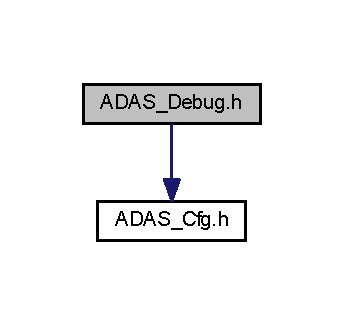
\includegraphics[width=165pt]{_a_d_a_s___debug_8h__incl}
\end{center}
\end{figure}
This graph shows which files directly or indirectly include this file\+:\nopagebreak
\begin{figure}[H]
\begin{center}
\leavevmode
\includegraphics[width=350pt]{_a_d_a_s___debug_8h__dep__incl}
\end{center}
\end{figure}
\subsection*{Macros}
\begin{DoxyCompactItemize}
\item 
\#define \mbox{\hyperlink{_a_d_a_s___debug_8h_ae33d310b25c222ae458b4a033d32b2ee}{D\+E\+B\+U\+G\+\_\+H}}
\item 
\#define \mbox{\hyperlink{_a_d_a_s___debug_8h_a57a35bfd7d13bdfab37a48171286ecee}{D\+P\+R\+I\+NT}}(...)
\item 
\#define \mbox{\hyperlink{_a_d_a_s___debug_8h_a39540ced659a9b6dfd1d185b695bd431}{D\+P\+R\+I\+N\+T\+LN}}(...)
\item 
\#define \mbox{\hyperlink{_a_d_a_s___debug_8h_aca77bd275e00af8a3eea089b7b0e6320}{D\+P\+R\+I\+N\+T2}}(...)~Serial.\+print(\+\_\+\+\_\+\+V\+A\+\_\+\+A\+R\+G\+S\+\_\+\+\_\+)
\item 
\#define \mbox{\hyperlink{_a_d_a_s___debug_8h_a5ef4c9f6c4e44b4b642a7893193f16ec}{D\+P\+R\+I\+N\+T\+L\+N2}}(...)~Serial.\+println(\+\_\+\+\_\+\+V\+A\+\_\+\+A\+R\+G\+S\+\_\+\+\_\+)
\end{DoxyCompactItemize}


\subsection{Detailed Description}
This file contains redefinition of the serial functions for debugging purpose. 

\begin{DoxyAuthor}{Author}
Christoph Jurczyk 
\end{DoxyAuthor}
\begin{DoxyDate}{Date}
January 29, 2019 
\end{DoxyDate}


\subsection{Macro Definition Documentation}
\mbox{\Hypertarget{_a_d_a_s___debug_8h_ae33d310b25c222ae458b4a033d32b2ee}\label{_a_d_a_s___debug_8h_ae33d310b25c222ae458b4a033d32b2ee}} 
\index{ADAS\_Debug.h@{ADAS\_Debug.h}!DEBUG\_H@{DEBUG\_H}}
\index{DEBUG\_H@{DEBUG\_H}!ADAS\_Debug.h@{ADAS\_Debug.h}}
\subsubsection{\texorpdfstring{DEBUG\_H}{DEBUG\_H}}
{\footnotesize\ttfamily \#define D\+E\+B\+U\+G\+\_\+H}



Definition at line 12 of file A\+D\+A\+S\+\_\+\+Debug.\+h.

\mbox{\Hypertarget{_a_d_a_s___debug_8h_a57a35bfd7d13bdfab37a48171286ecee}\label{_a_d_a_s___debug_8h_a57a35bfd7d13bdfab37a48171286ecee}} 
\index{ADAS\_Debug.h@{ADAS\_Debug.h}!DPRINT@{DPRINT}}
\index{DPRINT@{DPRINT}!ADAS\_Debug.h@{ADAS\_Debug.h}}
\subsubsection{\texorpdfstring{DPRINT}{DPRINT}}
{\footnotesize\ttfamily \#define D\+P\+R\+I\+NT(\begin{DoxyParamCaption}\item[{}]{... }\end{DoxyParamCaption})}

Debug enabled\+: remap D\+P\+R\+I\+NT and D\+P\+R\+I\+N\+T\+LN to Serial functions 

Definition at line 27 of file A\+D\+A\+S\+\_\+\+Debug.\+h.

\mbox{\Hypertarget{_a_d_a_s___debug_8h_aca77bd275e00af8a3eea089b7b0e6320}\label{_a_d_a_s___debug_8h_aca77bd275e00af8a3eea089b7b0e6320}} 
\index{ADAS\_Debug.h@{ADAS\_Debug.h}!DPRINT2@{DPRINT2}}
\index{DPRINT2@{DPRINT2}!ADAS\_Debug.h@{ADAS\_Debug.h}}
\subsubsection{\texorpdfstring{DPRINT2}{DPRINT2}}
{\footnotesize\ttfamily \#define D\+P\+R\+I\+N\+T2(\begin{DoxyParamCaption}\item[{}]{... }\end{DoxyParamCaption})~Serial.\+print(\+\_\+\+\_\+\+V\+A\+\_\+\+A\+R\+G\+S\+\_\+\+\_\+)}



Definition at line 33 of file A\+D\+A\+S\+\_\+\+Debug.\+h.

\mbox{\Hypertarget{_a_d_a_s___debug_8h_a39540ced659a9b6dfd1d185b695bd431}\label{_a_d_a_s___debug_8h_a39540ced659a9b6dfd1d185b695bd431}} 
\index{ADAS\_Debug.h@{ADAS\_Debug.h}!DPRINTLN@{DPRINTLN}}
\index{DPRINTLN@{DPRINTLN}!ADAS\_Debug.h@{ADAS\_Debug.h}}
\subsubsection{\texorpdfstring{DPRINTLN}{DPRINTLN}}
{\footnotesize\ttfamily \#define D\+P\+R\+I\+N\+T\+LN(\begin{DoxyParamCaption}\item[{}]{... }\end{DoxyParamCaption})}



Definition at line 28 of file A\+D\+A\+S\+\_\+\+Debug.\+h.

\mbox{\Hypertarget{_a_d_a_s___debug_8h_a5ef4c9f6c4e44b4b642a7893193f16ec}\label{_a_d_a_s___debug_8h_a5ef4c9f6c4e44b4b642a7893193f16ec}} 
\index{ADAS\_Debug.h@{ADAS\_Debug.h}!DPRINTLN2@{DPRINTLN2}}
\index{DPRINTLN2@{DPRINTLN2}!ADAS\_Debug.h@{ADAS\_Debug.h}}
\subsubsection{\texorpdfstring{DPRINTLN2}{DPRINTLN2}}
{\footnotesize\ttfamily \#define D\+P\+R\+I\+N\+T\+L\+N2(\begin{DoxyParamCaption}\item[{}]{... }\end{DoxyParamCaption})~Serial.\+println(\+\_\+\+\_\+\+V\+A\+\_\+\+A\+R\+G\+S\+\_\+\+\_\+)}



Definition at line 34 of file A\+D\+A\+S\+\_\+\+Debug.\+h.


\hypertarget{_a_d_a_s___m_c_u_8ino}{}\section{A\+D\+A\+S\+\_\+\+M\+C\+U.\+ino File Reference}
\label{_a_d_a_s___m_c_u_8ino}\index{A\+D\+A\+S\+\_\+\+M\+C\+U.\+ino@{A\+D\+A\+S\+\_\+\+M\+C\+U.\+ino}}


Main file for the NavU of the A\+D\+AS project.  


{\ttfamily \#include \char`\"{}A\+D\+A\+S\+\_\+\+Types.\+h\char`\"{}}\newline
{\ttfamily \#include \char`\"{}A\+D\+A\+S\+\_\+\+Cfg.\+h\char`\"{}}\newline
{\ttfamily \#include \char`\"{}A\+D\+A\+S\+\_\+\+Debug.\+h\char`\"{}}\newline
{\ttfamily \#include \char`\"{}Timer.\+h\char`\"{}}\newline
{\ttfamily \#include \char`\"{}H\+A\+L\+\_\+\+Drive\+Unit.\+h\char`\"{}}\newline
{\ttfamily \#include \char`\"{}H\+A\+L\+\_\+\+Encoder.\+h\char`\"{}}\newline
{\ttfamily \#include \char`\"{}H\+A\+L\+\_\+\+I\+M\+U.\+h\char`\"{}}\newline
{\ttfamily \#include \char`\"{}H\+A\+L\+\_\+\+P\+W\+M.\+h\char`\"{}}\newline
{\ttfamily \#include \char`\"{}H\+A\+L\+\_\+\+Serial\+\_\+\+I\+F.\+h\char`\"{}}\newline
{\ttfamily \#include \char`\"{}Comm\+\_\+\+Inertial.\+h\char`\"{}}\newline
{\ttfamily \#include \char`\"{}Comm\+\_\+\+I\+C\+C.\+h\char`\"{}}\newline
{\ttfamily \#include \char`\"{}App\+\_\+\+Motor\+Ctrl.\+h\char`\"{}}\newline
{\ttfamily \#include \char`\"{}App\+\_\+\+Stateflow.\+h\char`\"{}}\newline
{\ttfamily \#include \char`\"{}App\+\_\+\+Stateflowtypes.\+h\char`\"{}}\newline
Include dependency graph for A\+D\+A\+S\+\_\+\+M\+C\+U.\+ino\+:
\nopagebreak
\begin{figure}[H]
\begin{center}
\leavevmode
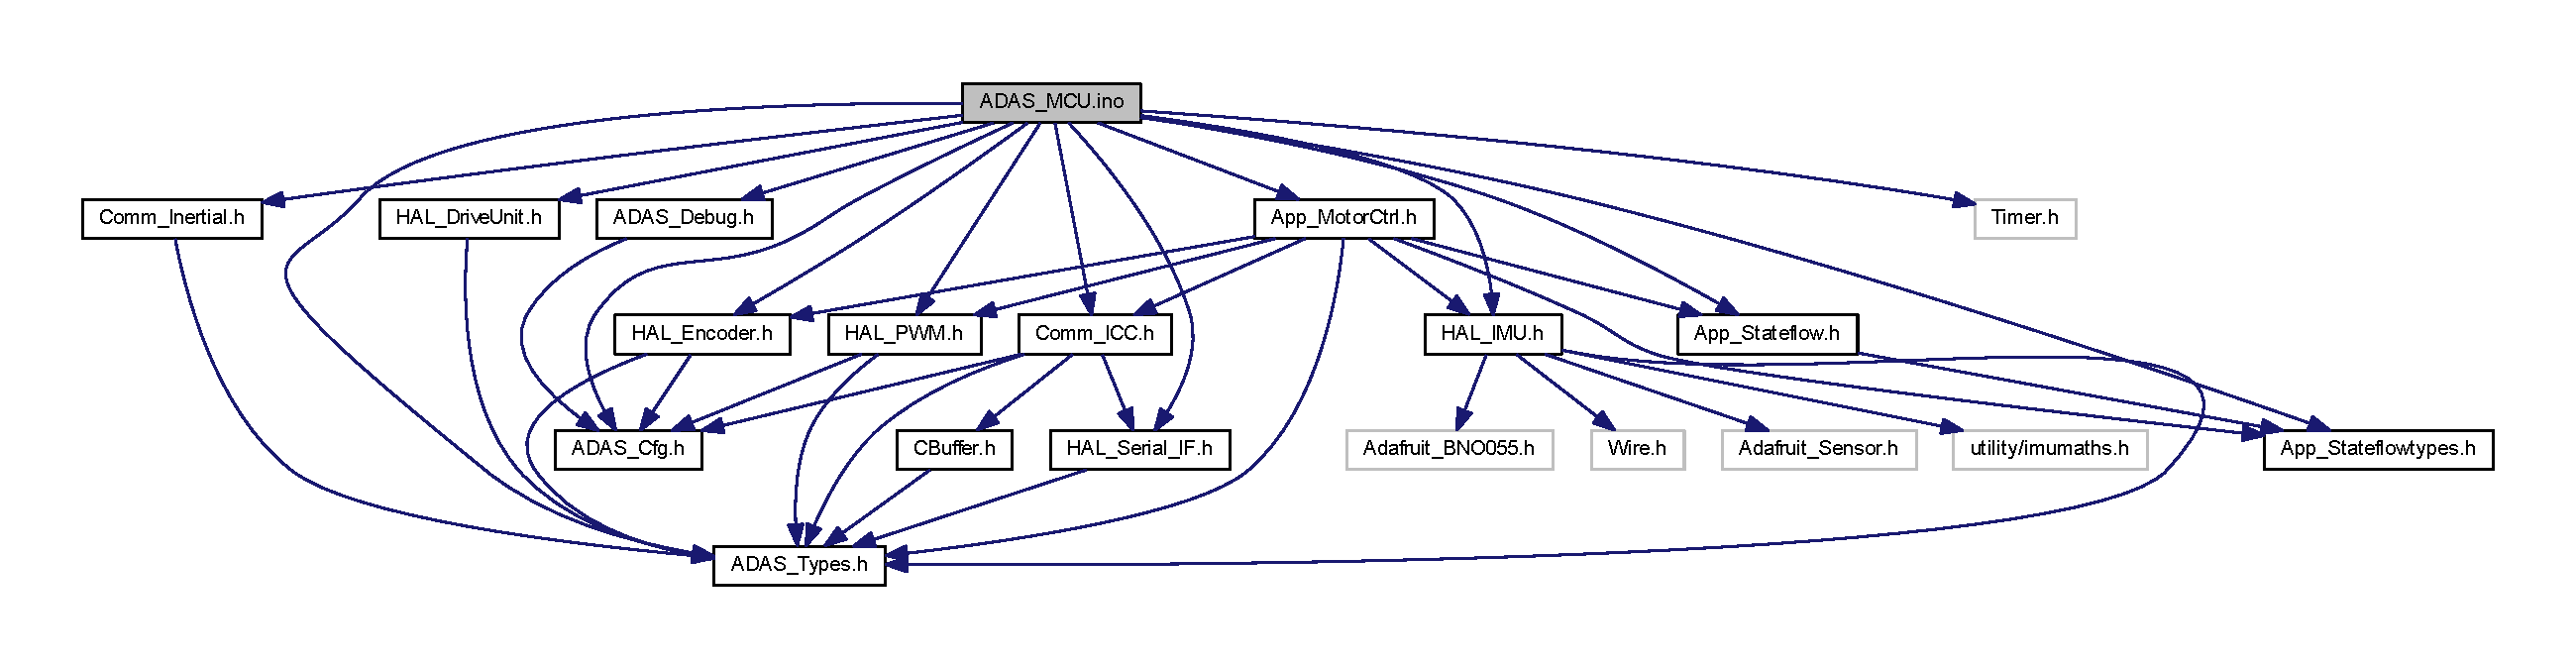
\includegraphics[width=350pt]{_a_d_a_s___m_c_u_8ino__incl}
\end{center}
\end{figure}
\subsection*{Functions}
\begin{DoxyCompactItemize}
\item 
void \mbox{\hyperlink{_a_d_a_s___m_c_u_8ino_a9f2f19081d81dba1b47615d1d9363281}{timer\+Callback}} (void $\ast$context)
\item 
void \mbox{\hyperlink{_a_d_a_s___m_c_u_8ino_a13fba9b7b9c02542e403a1142b5ad344}{Enc\+\_\+\+I\+S\+R\+\_\+R}} (void)
\item 
void \mbox{\hyperlink{_a_d_a_s___m_c_u_8ino_a89c135c3ad9390c0a5c08c78a9c985d1}{Enc\+\_\+\+I\+S\+R\+\_\+L}} (void)
\item 
void \mbox{\hyperlink{_a_d_a_s___m_c_u_8ino_a4fc01d736fe50cf5b977f755b675f11d}{setup}} ()
\item 
void \mbox{\hyperlink{_a_d_a_s___m_c_u_8ino_afe461d27b9c48d5921c00d521181f12f}{loop}} ()
\item 
\mbox{\hyperlink{_a_d_a_s___m_c_u_8ino_a63a86aad9ba2e355fe6380da553f554e}{I\+SR}} (U\+S\+A\+R\+T2\+\_\+\+R\+X\+\_\+vect)
\end{DoxyCompactItemize}
\subsection*{Variables}
\begin{DoxyCompactItemize}
\item 
Timer \mbox{\hyperlink{_a_d_a_s___m_c_u_8ino_a978d88b393c8a37dc2614c88788b3442}{t}}
\item 
\mbox{\hyperlink{class_c_i_m_u_unit}{C\+I\+M\+U\+Unit}} \mbox{\hyperlink{_a_d_a_s___m_c_u_8ino_ae51e36f83228f859afeb8a72e60339a6}{imu\+\_\+o}}
\item 
\mbox{\hyperlink{class_c_encoder}{C\+Encoder}} \mbox{\hyperlink{_a_d_a_s___m_c_u_8ino_ad90699f8fbb0fa8f734ae5c30885ee3b}{enc1\+\_\+o}} (\mbox{\hyperlink{class_c_encoder_a49810cc352199fb02a60e2ef8ac6cbc3a8f0ceb6874e0c79b53bf26fa42a1b652}{C\+Encoder\+::\+E1}})
\item 
\mbox{\hyperlink{class_c_encoder}{C\+Encoder}} \mbox{\hyperlink{_a_d_a_s___m_c_u_8ino_a54cfc96aae4913b87ab356a0665557a5}{enc2\+\_\+o}} (\mbox{\hyperlink{class_c_encoder_a49810cc352199fb02a60e2ef8ac6cbc3aaa314a69656e242defabd33eb8e90284}{C\+Encoder\+::\+E2}})
\item 
\mbox{\hyperlink{class_c_p_w_m_unit}{C\+P\+W\+M\+Unit}} \mbox{\hyperlink{_a_d_a_s___m_c_u_8ino_a10a570a59ef56c08699c4fec61d47d16}{pwm\+Unit\+Left\+\_\+o}} (\mbox{\hyperlink{class_c_p_w_m_unit_ad3e55d1df0367d8a090d4b835704be44a3f6167a7882e80f1ad05c8bff5e538c0}{C\+P\+W\+M\+Unit\+::\+P\+W\+M1}})
\item 
\mbox{\hyperlink{class_c_p_w_m_unit}{C\+P\+W\+M\+Unit}} \mbox{\hyperlink{_a_d_a_s___m_c_u_8ino_a49af1ef8724d9cb785e37641bb0cdc6b}{pwm\+Unit\+Right\+\_\+o}} (\mbox{\hyperlink{class_c_p_w_m_unit_ad3e55d1df0367d8a090d4b835704be44afc7888ea63be5da5551d10db3d676185}{C\+P\+W\+M\+Unit\+::\+P\+W\+M2}})
\item 
\mbox{\hyperlink{class_c_serial}{C\+Serial}} \mbox{\hyperlink{_a_d_a_s___m_c_u_8ino_ad1e6d9fed4369104e412a46c019634d2}{icc\+Port}} (\mbox{\hyperlink{class_c_serial_a000039540cc90b18bafacf5744e7eda2a8cc95f4591147b0df028e003f82220a1}{C\+Serial\+::\+S2}}, \mbox{\hyperlink{_a_d_a_s___cfg_8h_abf41bed56ee0b2a8858687c4420bb110}{I\+C\+C\+\_\+\+R\+C\+V\+\_\+\+B\+U\+F\+F\+\_\+\+S\+I\+ZE}})
\item 
\mbox{\hyperlink{class_c_i_c_c_comms}{C\+I\+C\+C\+Comms}} \mbox{\hyperlink{_a_d_a_s___m_c_u_8ino_a62ef6b3308259edb69af585549178324}{icc\+Comms\+\_\+o}} (\mbox{\hyperlink{_a_d_a_s___m_c_u_8ino_ad1e6d9fed4369104e412a46c019634d2}{icc\+Port}})
\item 
\mbox{\hyperlink{class_c_motor_ctrl}{C\+Motor\+Ctrl}} \mbox{\hyperlink{_a_d_a_s___m_c_u_8ino_a60ac8587f0c0967b5e3056da59168874}{m\+Ctrl\+\_\+o}} (\mbox{\hyperlink{_a_d_a_s___m_c_u_8ino_ae51e36f83228f859afeb8a72e60339a6}{imu\+\_\+o}}, \mbox{\hyperlink{_a_d_a_s___m_c_u_8ino_a10a570a59ef56c08699c4fec61d47d16}{pwm\+Unit\+Left\+\_\+o}}, \mbox{\hyperlink{_a_d_a_s___m_c_u_8ino_a49af1ef8724d9cb785e37641bb0cdc6b}{pwm\+Unit\+Right\+\_\+o}}, \mbox{\hyperlink{_a_d_a_s___m_c_u_8ino_ad90699f8fbb0fa8f734ae5c30885ee3b}{enc1\+\_\+o}}, \mbox{\hyperlink{_a_d_a_s___m_c_u_8ino_a54cfc96aae4913b87ab356a0665557a5}{enc2\+\_\+o}}, \mbox{\hyperlink{_a_d_a_s___m_c_u_8ino_a62ef6b3308259edb69af585549178324}{icc\+Comms\+\_\+o}})
\end{DoxyCompactItemize}


\subsection{Detailed Description}
Main file for the NavU of the A\+D\+AS project. 

\begin{DoxyAuthor}{Author}
Hannes Baehr, Juliane Mueller 
\end{DoxyAuthor}
\begin{DoxyDate}{Date}
January 29, 2019 
\end{DoxyDate}


\subsection{Function Documentation}
\mbox{\Hypertarget{_a_d_a_s___m_c_u_8ino_a89c135c3ad9390c0a5c08c78a9c985d1}\label{_a_d_a_s___m_c_u_8ino_a89c135c3ad9390c0a5c08c78a9c985d1}} 
\index{A\+D\+A\+S\+\_\+\+M\+C\+U.\+ino@{A\+D\+A\+S\+\_\+\+M\+C\+U.\+ino}!Enc\+\_\+\+I\+S\+R\+\_\+L@{Enc\+\_\+\+I\+S\+R\+\_\+L}}
\index{Enc\+\_\+\+I\+S\+R\+\_\+L@{Enc\+\_\+\+I\+S\+R\+\_\+L}!A\+D\+A\+S\+\_\+\+M\+C\+U.\+ino@{A\+D\+A\+S\+\_\+\+M\+C\+U.\+ino}}
\subsubsection{\texorpdfstring{Enc\+\_\+\+I\+S\+R\+\_\+\+L()}{Enc\_ISR\_L()}}
{\footnotesize\ttfamily void Enc\+\_\+\+I\+S\+R\+\_\+L (\begin{DoxyParamCaption}\item[{void}]{ }\end{DoxyParamCaption})}



Definition at line 87 of file A\+D\+A\+S\+\_\+\+M\+C\+U.\+ino.

Here is the call graph for this function\+:
\nopagebreak
\begin{figure}[H]
\begin{center}
\leavevmode
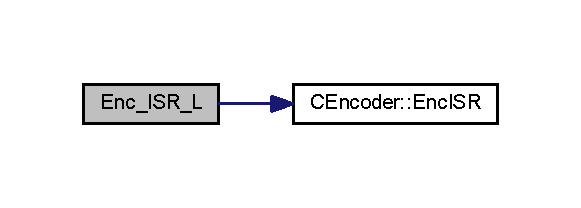
\includegraphics[width=279pt]{_a_d_a_s___m_c_u_8ino_a89c135c3ad9390c0a5c08c78a9c985d1_cgraph}
\end{center}
\end{figure}
Here is the caller graph for this function\+:
\nopagebreak
\begin{figure}[H]
\begin{center}
\leavevmode
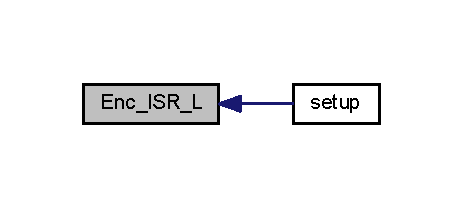
\includegraphics[width=222pt]{_a_d_a_s___m_c_u_8ino_a89c135c3ad9390c0a5c08c78a9c985d1_icgraph}
\end{center}
\end{figure}
\mbox{\Hypertarget{_a_d_a_s___m_c_u_8ino_a13fba9b7b9c02542e403a1142b5ad344}\label{_a_d_a_s___m_c_u_8ino_a13fba9b7b9c02542e403a1142b5ad344}} 
\index{A\+D\+A\+S\+\_\+\+M\+C\+U.\+ino@{A\+D\+A\+S\+\_\+\+M\+C\+U.\+ino}!Enc\+\_\+\+I\+S\+R\+\_\+R@{Enc\+\_\+\+I\+S\+R\+\_\+R}}
\index{Enc\+\_\+\+I\+S\+R\+\_\+R@{Enc\+\_\+\+I\+S\+R\+\_\+R}!A\+D\+A\+S\+\_\+\+M\+C\+U.\+ino@{A\+D\+A\+S\+\_\+\+M\+C\+U.\+ino}}
\subsubsection{\texorpdfstring{Enc\+\_\+\+I\+S\+R\+\_\+\+R()}{Enc\_ISR\_R()}}
{\footnotesize\ttfamily void Enc\+\_\+\+I\+S\+R\+\_\+R (\begin{DoxyParamCaption}\item[{void}]{ }\end{DoxyParamCaption})}



Definition at line 83 of file A\+D\+A\+S\+\_\+\+M\+C\+U.\+ino.

Here is the call graph for this function\+:
\nopagebreak
\begin{figure}[H]
\begin{center}
\leavevmode
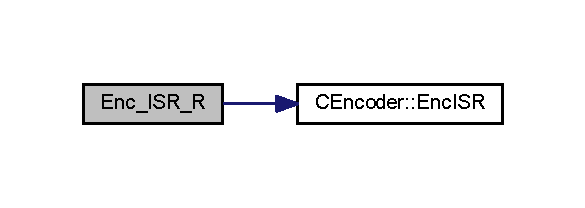
\includegraphics[width=281pt]{_a_d_a_s___m_c_u_8ino_a13fba9b7b9c02542e403a1142b5ad344_cgraph}
\end{center}
\end{figure}
Here is the caller graph for this function\+:
\nopagebreak
\begin{figure}[H]
\begin{center}
\leavevmode
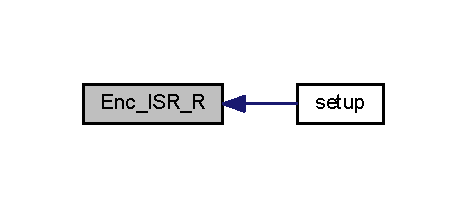
\includegraphics[width=224pt]{_a_d_a_s___m_c_u_8ino_a13fba9b7b9c02542e403a1142b5ad344_icgraph}
\end{center}
\end{figure}
\mbox{\Hypertarget{_a_d_a_s___m_c_u_8ino_a63a86aad9ba2e355fe6380da553f554e}\label{_a_d_a_s___m_c_u_8ino_a63a86aad9ba2e355fe6380da553f554e}} 
\index{A\+D\+A\+S\+\_\+\+M\+C\+U.\+ino@{A\+D\+A\+S\+\_\+\+M\+C\+U.\+ino}!I\+SR@{I\+SR}}
\index{I\+SR@{I\+SR}!A\+D\+A\+S\+\_\+\+M\+C\+U.\+ino@{A\+D\+A\+S\+\_\+\+M\+C\+U.\+ino}}
\subsubsection{\texorpdfstring{I\+S\+R()}{ISR()}}
{\footnotesize\ttfamily I\+SR (\begin{DoxyParamCaption}\item[{U\+S\+A\+R\+T2\+\_\+\+R\+X\+\_\+vect}]{ }\end{DoxyParamCaption})}



Definition at line 73 of file A\+D\+A\+S\+\_\+\+M\+C\+U.\+ino.

Here is the call graph for this function\+:
\nopagebreak
\begin{figure}[H]
\begin{center}
\leavevmode
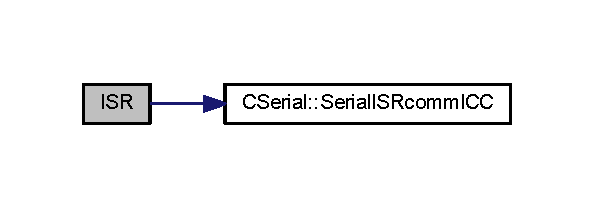
\includegraphics[width=285pt]{_a_d_a_s___m_c_u_8ino_a63a86aad9ba2e355fe6380da553f554e_cgraph}
\end{center}
\end{figure}
\mbox{\Hypertarget{_a_d_a_s___m_c_u_8ino_afe461d27b9c48d5921c00d521181f12f}\label{_a_d_a_s___m_c_u_8ino_afe461d27b9c48d5921c00d521181f12f}} 
\index{A\+D\+A\+S\+\_\+\+M\+C\+U.\+ino@{A\+D\+A\+S\+\_\+\+M\+C\+U.\+ino}!loop@{loop}}
\index{loop@{loop}!A\+D\+A\+S\+\_\+\+M\+C\+U.\+ino@{A\+D\+A\+S\+\_\+\+M\+C\+U.\+ino}}
\subsubsection{\texorpdfstring{loop()}{loop()}}
{\footnotesize\ttfamily void loop (\begin{DoxyParamCaption}{ }\end{DoxyParamCaption})}



Definition at line 66 of file A\+D\+A\+S\+\_\+\+M\+C\+U.\+ino.

Here is the call graph for this function\+:
\nopagebreak
\begin{figure}[H]
\begin{center}
\leavevmode
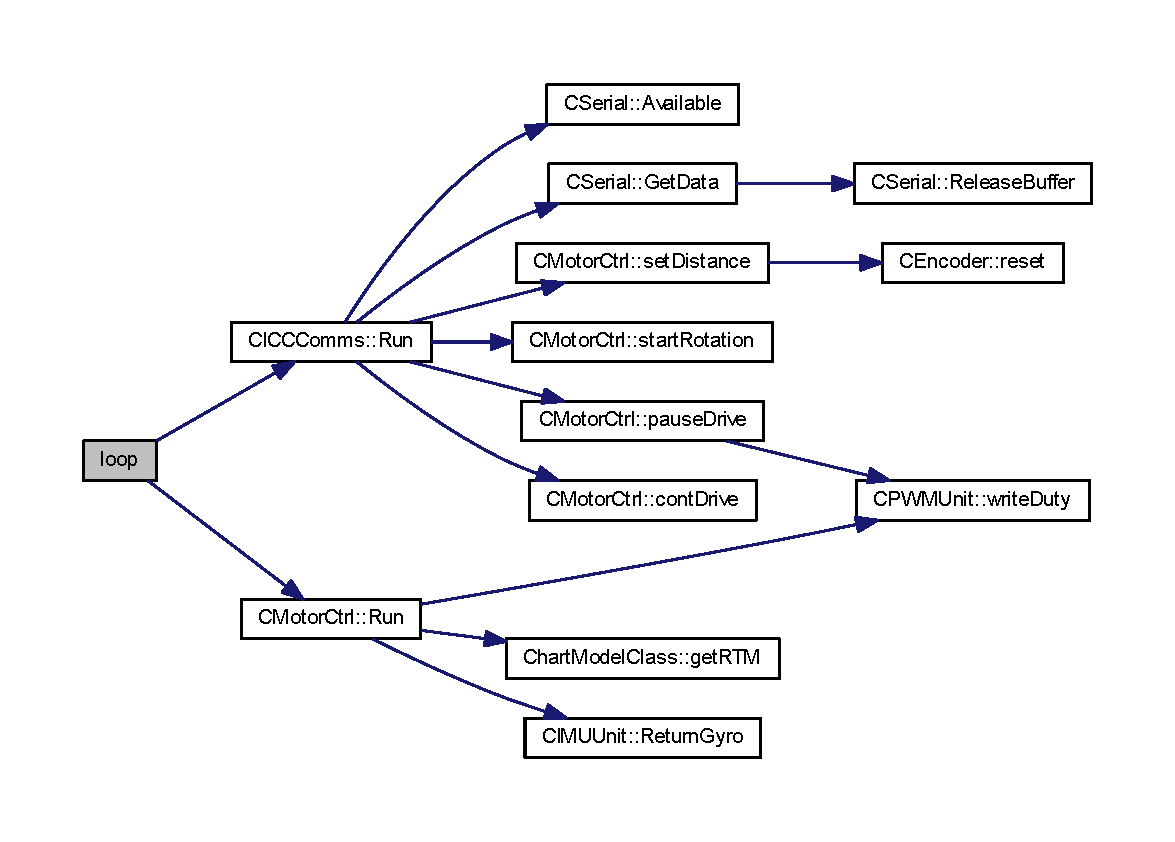
\includegraphics[width=350pt]{_a_d_a_s___m_c_u_8ino_afe461d27b9c48d5921c00d521181f12f_cgraph}
\end{center}
\end{figure}
\mbox{\Hypertarget{_a_d_a_s___m_c_u_8ino_a4fc01d736fe50cf5b977f755b675f11d}\label{_a_d_a_s___m_c_u_8ino_a4fc01d736fe50cf5b977f755b675f11d}} 
\index{A\+D\+A\+S\+\_\+\+M\+C\+U.\+ino@{A\+D\+A\+S\+\_\+\+M\+C\+U.\+ino}!setup@{setup}}
\index{setup@{setup}!A\+D\+A\+S\+\_\+\+M\+C\+U.\+ino@{A\+D\+A\+S\+\_\+\+M\+C\+U.\+ino}}
\subsubsection{\texorpdfstring{setup()}{setup()}}
{\footnotesize\ttfamily void setup (\begin{DoxyParamCaption}{ }\end{DoxyParamCaption})}



Definition at line 52 of file A\+D\+A\+S\+\_\+\+M\+C\+U.\+ino.

Here is the call graph for this function\+:
\nopagebreak
\begin{figure}[H]
\begin{center}
\leavevmode
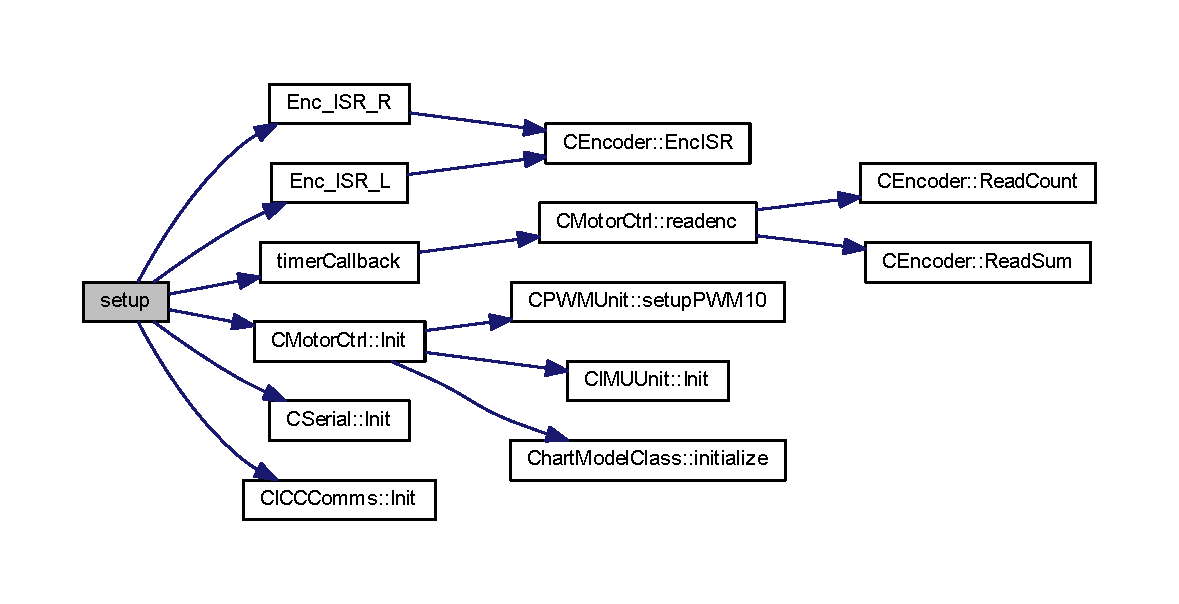
\includegraphics[width=350pt]{_a_d_a_s___m_c_u_8ino_a4fc01d736fe50cf5b977f755b675f11d_cgraph}
\end{center}
\end{figure}
\mbox{\Hypertarget{_a_d_a_s___m_c_u_8ino_a9f2f19081d81dba1b47615d1d9363281}\label{_a_d_a_s___m_c_u_8ino_a9f2f19081d81dba1b47615d1d9363281}} 
\index{A\+D\+A\+S\+\_\+\+M\+C\+U.\+ino@{A\+D\+A\+S\+\_\+\+M\+C\+U.\+ino}!timer\+Callback@{timer\+Callback}}
\index{timer\+Callback@{timer\+Callback}!A\+D\+A\+S\+\_\+\+M\+C\+U.\+ino@{A\+D\+A\+S\+\_\+\+M\+C\+U.\+ino}}
\subsubsection{\texorpdfstring{timer\+Callback()}{timerCallback()}}
{\footnotesize\ttfamily void timer\+Callback (\begin{DoxyParamCaption}\item[{void $\ast$}]{context }\end{DoxyParamCaption})}



Definition at line 79 of file A\+D\+A\+S\+\_\+\+M\+C\+U.\+ino.

Here is the call graph for this function\+:
\nopagebreak
\begin{figure}[H]
\begin{center}
\leavevmode
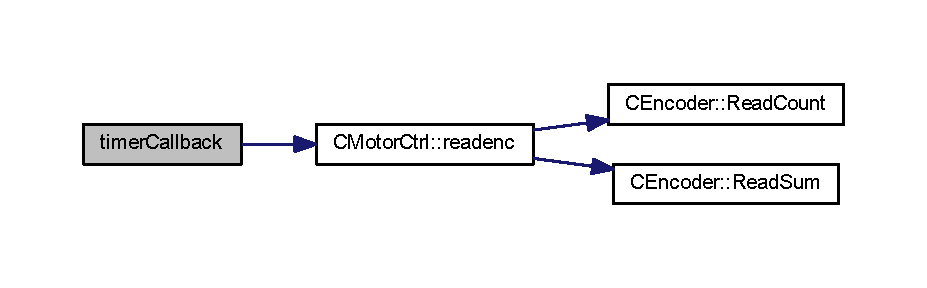
\includegraphics[width=350pt]{_a_d_a_s___m_c_u_8ino_a9f2f19081d81dba1b47615d1d9363281_cgraph}
\end{center}
\end{figure}
Here is the caller graph for this function\+:
\nopagebreak
\begin{figure}[H]
\begin{center}
\leavevmode
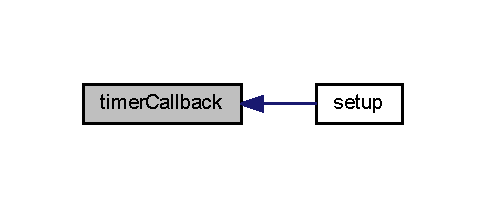
\includegraphics[width=233pt]{_a_d_a_s___m_c_u_8ino_a9f2f19081d81dba1b47615d1d9363281_icgraph}
\end{center}
\end{figure}


\subsection{Variable Documentation}
\mbox{\Hypertarget{_a_d_a_s___m_c_u_8ino_ad90699f8fbb0fa8f734ae5c30885ee3b}\label{_a_d_a_s___m_c_u_8ino_ad90699f8fbb0fa8f734ae5c30885ee3b}} 
\index{A\+D\+A\+S\+\_\+\+M\+C\+U.\+ino@{A\+D\+A\+S\+\_\+\+M\+C\+U.\+ino}!enc1\+\_\+o@{enc1\+\_\+o}}
\index{enc1\+\_\+o@{enc1\+\_\+o}!A\+D\+A\+S\+\_\+\+M\+C\+U.\+ino@{A\+D\+A\+S\+\_\+\+M\+C\+U.\+ino}}
\subsubsection{\texorpdfstring{enc1\+\_\+o}{enc1\_o}}
{\footnotesize\ttfamily \mbox{\hyperlink{class_c_encoder}{C\+Encoder}} enc1\+\_\+o(\mbox{\hyperlink{class_c_encoder_a49810cc352199fb02a60e2ef8ac6cbc3a8f0ceb6874e0c79b53bf26fa42a1b652}{C\+Encoder\+::\+E1}})}

\mbox{\Hypertarget{_a_d_a_s___m_c_u_8ino_a54cfc96aae4913b87ab356a0665557a5}\label{_a_d_a_s___m_c_u_8ino_a54cfc96aae4913b87ab356a0665557a5}} 
\index{A\+D\+A\+S\+\_\+\+M\+C\+U.\+ino@{A\+D\+A\+S\+\_\+\+M\+C\+U.\+ino}!enc2\+\_\+o@{enc2\+\_\+o}}
\index{enc2\+\_\+o@{enc2\+\_\+o}!A\+D\+A\+S\+\_\+\+M\+C\+U.\+ino@{A\+D\+A\+S\+\_\+\+M\+C\+U.\+ino}}
\subsubsection{\texorpdfstring{enc2\+\_\+o}{enc2\_o}}
{\footnotesize\ttfamily \mbox{\hyperlink{class_c_encoder}{C\+Encoder}} enc2\+\_\+o(\mbox{\hyperlink{class_c_encoder_a49810cc352199fb02a60e2ef8ac6cbc3aaa314a69656e242defabd33eb8e90284}{C\+Encoder\+::\+E2}})}

\mbox{\Hypertarget{_a_d_a_s___m_c_u_8ino_a62ef6b3308259edb69af585549178324}\label{_a_d_a_s___m_c_u_8ino_a62ef6b3308259edb69af585549178324}} 
\index{A\+D\+A\+S\+\_\+\+M\+C\+U.\+ino@{A\+D\+A\+S\+\_\+\+M\+C\+U.\+ino}!icc\+Comms\+\_\+o@{icc\+Comms\+\_\+o}}
\index{icc\+Comms\+\_\+o@{icc\+Comms\+\_\+o}!A\+D\+A\+S\+\_\+\+M\+C\+U.\+ino@{A\+D\+A\+S\+\_\+\+M\+C\+U.\+ino}}
\subsubsection{\texorpdfstring{icc\+Comms\+\_\+o}{iccComms\_o}}
{\footnotesize\ttfamily \mbox{\hyperlink{class_c_i_c_c_comms}{C\+I\+C\+C\+Comms}} icc\+Comms\+\_\+o(\mbox{\hyperlink{_a_d_a_s___m_c_u_8ino_ad1e6d9fed4369104e412a46c019634d2}{icc\+Port}})}

\mbox{\Hypertarget{_a_d_a_s___m_c_u_8ino_ad1e6d9fed4369104e412a46c019634d2}\label{_a_d_a_s___m_c_u_8ino_ad1e6d9fed4369104e412a46c019634d2}} 
\index{A\+D\+A\+S\+\_\+\+M\+C\+U.\+ino@{A\+D\+A\+S\+\_\+\+M\+C\+U.\+ino}!icc\+Port@{icc\+Port}}
\index{icc\+Port@{icc\+Port}!A\+D\+A\+S\+\_\+\+M\+C\+U.\+ino@{A\+D\+A\+S\+\_\+\+M\+C\+U.\+ino}}
\subsubsection{\texorpdfstring{icc\+Port}{iccPort}}
{\footnotesize\ttfamily \mbox{\hyperlink{class_c_serial}{C\+Serial}} icc\+Port(\mbox{\hyperlink{class_c_serial_a000039540cc90b18bafacf5744e7eda2a8cc95f4591147b0df028e003f82220a1}{C\+Serial\+::\+S2}}, \mbox{\hyperlink{_a_d_a_s___cfg_8h_abf41bed56ee0b2a8858687c4420bb110}{I\+C\+C\+\_\+\+R\+C\+V\+\_\+\+B\+U\+F\+F\+\_\+\+S\+I\+ZE}})}

\mbox{\Hypertarget{_a_d_a_s___m_c_u_8ino_ae51e36f83228f859afeb8a72e60339a6}\label{_a_d_a_s___m_c_u_8ino_ae51e36f83228f859afeb8a72e60339a6}} 
\index{A\+D\+A\+S\+\_\+\+M\+C\+U.\+ino@{A\+D\+A\+S\+\_\+\+M\+C\+U.\+ino}!imu\+\_\+o@{imu\+\_\+o}}
\index{imu\+\_\+o@{imu\+\_\+o}!A\+D\+A\+S\+\_\+\+M\+C\+U.\+ino@{A\+D\+A\+S\+\_\+\+M\+C\+U.\+ino}}
\subsubsection{\texorpdfstring{imu\+\_\+o}{imu\_o}}
{\footnotesize\ttfamily \mbox{\hyperlink{class_c_i_m_u_unit}{C\+I\+M\+U\+Unit}} imu\+\_\+o}



Definition at line 38 of file A\+D\+A\+S\+\_\+\+M\+C\+U.\+ino.

\mbox{\Hypertarget{_a_d_a_s___m_c_u_8ino_a60ac8587f0c0967b5e3056da59168874}\label{_a_d_a_s___m_c_u_8ino_a60ac8587f0c0967b5e3056da59168874}} 
\index{A\+D\+A\+S\+\_\+\+M\+C\+U.\+ino@{A\+D\+A\+S\+\_\+\+M\+C\+U.\+ino}!m\+Ctrl\+\_\+o@{m\+Ctrl\+\_\+o}}
\index{m\+Ctrl\+\_\+o@{m\+Ctrl\+\_\+o}!A\+D\+A\+S\+\_\+\+M\+C\+U.\+ino@{A\+D\+A\+S\+\_\+\+M\+C\+U.\+ino}}
\subsubsection{\texorpdfstring{m\+Ctrl\+\_\+o}{mCtrl\_o}}
{\footnotesize\ttfamily \mbox{\hyperlink{class_c_motor_ctrl}{C\+Motor\+Ctrl}} m\+Ctrl\+\_\+o(\mbox{\hyperlink{_a_d_a_s___m_c_u_8ino_ae51e36f83228f859afeb8a72e60339a6}{imu\+\_\+o}}, \mbox{\hyperlink{_a_d_a_s___m_c_u_8ino_a10a570a59ef56c08699c4fec61d47d16}{pwm\+Unit\+Left\+\_\+o}}, \mbox{\hyperlink{_a_d_a_s___m_c_u_8ino_a49af1ef8724d9cb785e37641bb0cdc6b}{pwm\+Unit\+Right\+\_\+o}}, \mbox{\hyperlink{_a_d_a_s___m_c_u_8ino_ad90699f8fbb0fa8f734ae5c30885ee3b}{enc1\+\_\+o}}, \mbox{\hyperlink{_a_d_a_s___m_c_u_8ino_a54cfc96aae4913b87ab356a0665557a5}{enc2\+\_\+o}}, \mbox{\hyperlink{_a_d_a_s___m_c_u_8ino_a62ef6b3308259edb69af585549178324}{icc\+Comms\+\_\+o}})}

\mbox{\Hypertarget{_a_d_a_s___m_c_u_8ino_a10a570a59ef56c08699c4fec61d47d16}\label{_a_d_a_s___m_c_u_8ino_a10a570a59ef56c08699c4fec61d47d16}} 
\index{A\+D\+A\+S\+\_\+\+M\+C\+U.\+ino@{A\+D\+A\+S\+\_\+\+M\+C\+U.\+ino}!pwm\+Unit\+Left\+\_\+o@{pwm\+Unit\+Left\+\_\+o}}
\index{pwm\+Unit\+Left\+\_\+o@{pwm\+Unit\+Left\+\_\+o}!A\+D\+A\+S\+\_\+\+M\+C\+U.\+ino@{A\+D\+A\+S\+\_\+\+M\+C\+U.\+ino}}
\subsubsection{\texorpdfstring{pwm\+Unit\+Left\+\_\+o}{pwmUnitLeft\_o}}
{\footnotesize\ttfamily \mbox{\hyperlink{class_c_p_w_m_unit}{C\+P\+W\+M\+Unit}} pwm\+Unit\+Left\+\_\+o(\mbox{\hyperlink{class_c_p_w_m_unit_ad3e55d1df0367d8a090d4b835704be44a3f6167a7882e80f1ad05c8bff5e538c0}{C\+P\+W\+M\+Unit\+::\+P\+W\+M1}})}

\mbox{\Hypertarget{_a_d_a_s___m_c_u_8ino_a49af1ef8724d9cb785e37641bb0cdc6b}\label{_a_d_a_s___m_c_u_8ino_a49af1ef8724d9cb785e37641bb0cdc6b}} 
\index{A\+D\+A\+S\+\_\+\+M\+C\+U.\+ino@{A\+D\+A\+S\+\_\+\+M\+C\+U.\+ino}!pwm\+Unit\+Right\+\_\+o@{pwm\+Unit\+Right\+\_\+o}}
\index{pwm\+Unit\+Right\+\_\+o@{pwm\+Unit\+Right\+\_\+o}!A\+D\+A\+S\+\_\+\+M\+C\+U.\+ino@{A\+D\+A\+S\+\_\+\+M\+C\+U.\+ino}}
\subsubsection{\texorpdfstring{pwm\+Unit\+Right\+\_\+o}{pwmUnitRight\_o}}
{\footnotesize\ttfamily \mbox{\hyperlink{class_c_p_w_m_unit}{C\+P\+W\+M\+Unit}} pwm\+Unit\+Right\+\_\+o(\mbox{\hyperlink{class_c_p_w_m_unit_ad3e55d1df0367d8a090d4b835704be44afc7888ea63be5da5551d10db3d676185}{C\+P\+W\+M\+Unit\+::\+P\+W\+M2}})}

\mbox{\Hypertarget{_a_d_a_s___m_c_u_8ino_a978d88b393c8a37dc2614c88788b3442}\label{_a_d_a_s___m_c_u_8ino_a978d88b393c8a37dc2614c88788b3442}} 
\index{A\+D\+A\+S\+\_\+\+M\+C\+U.\+ino@{A\+D\+A\+S\+\_\+\+M\+C\+U.\+ino}!t@{t}}
\index{t@{t}!A\+D\+A\+S\+\_\+\+M\+C\+U.\+ino@{A\+D\+A\+S\+\_\+\+M\+C\+U.\+ino}}
\subsubsection{\texorpdfstring{t}{t}}
{\footnotesize\ttfamily Timer t}

Basics Periperals Comms layer App Layer 

Definition at line 35 of file A\+D\+A\+S\+\_\+\+M\+C\+U.\+ino.


\hypertarget{_a_d_a_s___types_8h}{}\section{A\+D\+A\+S\+\_\+\+Types.\+h File Reference}
\label{_a_d_a_s___types_8h}\index{ADAS\_Types.h@{ADAS\_Types.h}}


internal datatype mapping file  


This graph shows which files directly or indirectly include this file\+:
\nopagebreak
\begin{figure}[H]
\begin{center}
\leavevmode
\includegraphics[width=350pt]{_a_d_a_s___types_8h__dep__incl}
\end{center}
\end{figure}
\subsection*{Typedefs}
\begin{DoxyCompactItemize}
\item 
typedef unsigned long \mbox{\hyperlink{_a_d_a_s___types_8h_a06896e8c53f721507066c079052171f8}{uint32\+\_\+t}}
\item 
typedef unsigned int \mbox{\hyperlink{_a_d_a_s___types_8h_a1f1825b69244eb3ad2c7165ddc99c956}{uint16\+\_\+t}}
\item 
typedef unsigned char \mbox{\hyperlink{_a_d_a_s___types_8h_aba7bc1797add20fe3efdf37ced1182c5}{uint8\+\_\+t}}
\item 
typedef signed long \mbox{\hyperlink{_a_d_a_s___types_8h_a73705d44e0ddde601ded7d759dd0eaed}{sint32\+\_\+t}}
\item 
typedef signed int \mbox{\hyperlink{_a_d_a_s___types_8h_ae4c9b951dbb7355563c313abca5e2e75}{sint16\+\_\+t}}
\item 
typedef signed char \mbox{\hyperlink{_a_d_a_s___types_8h_a54cceacffb6d6dff03bf69f786d431a9}{sint8\+\_\+t}}
\item 
typedef float \mbox{\hyperlink{_a_d_a_s___types_8h_a4611b605e45ab401f02cab15c5e38715}{float32\+\_\+t}}
\item 
typedef double \mbox{\hyperlink{_a_d_a_s___types_8h_ac55f3ae81b5bc9053760baacf57e47f4}{float64\+\_\+t}}
\end{DoxyCompactItemize}


\subsection{Detailed Description}
internal datatype mapping file 

\begin{DoxyAuthor}{Author}
Aju Antony Jose 
\end{DoxyAuthor}
\begin{DoxyDate}{Date}
January 30, 2019 
\end{DoxyDate}


\subsection{Typedef Documentation}
\mbox{\Hypertarget{_a_d_a_s___types_8h_a4611b605e45ab401f02cab15c5e38715}\label{_a_d_a_s___types_8h_a4611b605e45ab401f02cab15c5e38715}} 
\index{ADAS\_Types.h@{ADAS\_Types.h}!float32\_t@{float32\_t}}
\index{float32\_t@{float32\_t}!ADAS\_Types.h@{ADAS\_Types.h}}
\subsubsection{\texorpdfstring{float32\_t}{float32\_t}}
{\footnotesize\ttfamily typedef float \mbox{\hyperlink{_a_d_a_s___types_8h_a4611b605e45ab401f02cab15c5e38715}{float32\+\_\+t}}}

type mapping 4 byte floating value 

Definition at line 24 of file A\+D\+A\+S\+\_\+\+Types.\+h.

\mbox{\Hypertarget{_a_d_a_s___types_8h_ac55f3ae81b5bc9053760baacf57e47f4}\label{_a_d_a_s___types_8h_ac55f3ae81b5bc9053760baacf57e47f4}} 
\index{ADAS\_Types.h@{ADAS\_Types.h}!float64\_t@{float64\_t}}
\index{float64\_t@{float64\_t}!ADAS\_Types.h@{ADAS\_Types.h}}
\subsubsection{\texorpdfstring{float64\_t}{float64\_t}}
{\footnotesize\ttfamily typedef double \mbox{\hyperlink{_a_d_a_s___types_8h_ac55f3ae81b5bc9053760baacf57e47f4}{float64\+\_\+t}}}

type mapping 8 byte floating value 

Definition at line 25 of file A\+D\+A\+S\+\_\+\+Types.\+h.

\mbox{\Hypertarget{_a_d_a_s___types_8h_ae4c9b951dbb7355563c313abca5e2e75}\label{_a_d_a_s___types_8h_ae4c9b951dbb7355563c313abca5e2e75}} 
\index{ADAS\_Types.h@{ADAS\_Types.h}!sint16\_t@{sint16\_t}}
\index{sint16\_t@{sint16\_t}!ADAS\_Types.h@{ADAS\_Types.h}}
\subsubsection{\texorpdfstring{sint16\_t}{sint16\_t}}
{\footnotesize\ttfamily typedef signed int \mbox{\hyperlink{_a_d_a_s___types_8h_ae4c9b951dbb7355563c313abca5e2e75}{sint16\+\_\+t}}}

type mapping signed 2 byte 

Definition at line 19 of file A\+D\+A\+S\+\_\+\+Types.\+h.

\mbox{\Hypertarget{_a_d_a_s___types_8h_a73705d44e0ddde601ded7d759dd0eaed}\label{_a_d_a_s___types_8h_a73705d44e0ddde601ded7d759dd0eaed}} 
\index{ADAS\_Types.h@{ADAS\_Types.h}!sint32\_t@{sint32\_t}}
\index{sint32\_t@{sint32\_t}!ADAS\_Types.h@{ADAS\_Types.h}}
\subsubsection{\texorpdfstring{sint32\_t}{sint32\_t}}
{\footnotesize\ttfamily typedef signed long \mbox{\hyperlink{_a_d_a_s___types_8h_a73705d44e0ddde601ded7d759dd0eaed}{sint32\+\_\+t}}}

type mapping signed 4 byte 

Definition at line 18 of file A\+D\+A\+S\+\_\+\+Types.\+h.

\mbox{\Hypertarget{_a_d_a_s___types_8h_a54cceacffb6d6dff03bf69f786d431a9}\label{_a_d_a_s___types_8h_a54cceacffb6d6dff03bf69f786d431a9}} 
\index{ADAS\_Types.h@{ADAS\_Types.h}!sint8\_t@{sint8\_t}}
\index{sint8\_t@{sint8\_t}!ADAS\_Types.h@{ADAS\_Types.h}}
\subsubsection{\texorpdfstring{sint8\_t}{sint8\_t}}
{\footnotesize\ttfamily typedef signed char \mbox{\hyperlink{_a_d_a_s___types_8h_a54cceacffb6d6dff03bf69f786d431a9}{sint8\+\_\+t}}}

type mapping signed 1 byte 

Definition at line 20 of file A\+D\+A\+S\+\_\+\+Types.\+h.

\mbox{\Hypertarget{_a_d_a_s___types_8h_a1f1825b69244eb3ad2c7165ddc99c956}\label{_a_d_a_s___types_8h_a1f1825b69244eb3ad2c7165ddc99c956}} 
\index{ADAS\_Types.h@{ADAS\_Types.h}!uint16\_t@{uint16\_t}}
\index{uint16\_t@{uint16\_t}!ADAS\_Types.h@{ADAS\_Types.h}}
\subsubsection{\texorpdfstring{uint16\_t}{uint16\_t}}
{\footnotesize\ttfamily typedef unsigned int \mbox{\hyperlink{_a_d_a_s___types_8h_a1f1825b69244eb3ad2c7165ddc99c956}{uint16\+\_\+t}}}

type mapping unsigned 2 byte 

Definition at line 14 of file A\+D\+A\+S\+\_\+\+Types.\+h.

\mbox{\Hypertarget{_a_d_a_s___types_8h_a06896e8c53f721507066c079052171f8}\label{_a_d_a_s___types_8h_a06896e8c53f721507066c079052171f8}} 
\index{ADAS\_Types.h@{ADAS\_Types.h}!uint32\_t@{uint32\_t}}
\index{uint32\_t@{uint32\_t}!ADAS\_Types.h@{ADAS\_Types.h}}
\subsubsection{\texorpdfstring{uint32\_t}{uint32\_t}}
{\footnotesize\ttfamily typedef unsigned long \mbox{\hyperlink{_a_d_a_s___types_8h_a06896e8c53f721507066c079052171f8}{uint32\+\_\+t}}}

type mapping unsigned 4 byte 

Definition at line 13 of file A\+D\+A\+S\+\_\+\+Types.\+h.

\mbox{\Hypertarget{_a_d_a_s___types_8h_aba7bc1797add20fe3efdf37ced1182c5}\label{_a_d_a_s___types_8h_aba7bc1797add20fe3efdf37ced1182c5}} 
\index{ADAS\_Types.h@{ADAS\_Types.h}!uint8\_t@{uint8\_t}}
\index{uint8\_t@{uint8\_t}!ADAS\_Types.h@{ADAS\_Types.h}}
\subsubsection{\texorpdfstring{uint8\_t}{uint8\_t}}
{\footnotesize\ttfamily typedef unsigned char \mbox{\hyperlink{_a_d_a_s___types_8h_aba7bc1797add20fe3efdf37ced1182c5}{uint8\+\_\+t}}}

type mapping unsigned 1 byte 

Definition at line 15 of file A\+D\+A\+S\+\_\+\+Types.\+h.


\hypertarget{_app___motor_ctrl_8cpp}{}\section{App\+\_\+\+Motor\+Ctrl.\+cpp File Reference}
\label{_app___motor_ctrl_8cpp}\index{App\+\_\+\+Motor\+Ctrl.\+cpp@{App\+\_\+\+Motor\+Ctrl.\+cpp}}


Application file for environmental data.  


{\ttfamily \#include \char`\"{}App\+\_\+\+Motor\+Ctrl.\+h\char`\"{}}\newline
{\ttfamily \#include \char`\"{}Arduino.\+h\char`\"{}}\newline
{\ttfamily \#include \char`\"{}H\+A\+L\+\_\+\+P\+W\+M.\+h\char`\"{}}\newline
{\ttfamily \#include \char`\"{}H\+A\+L\+\_\+\+I\+M\+U.\+h\char`\"{}}\newline
{\ttfamily \#include \char`\"{}App\+\_\+\+Stateflow.\+h\char`\"{}}\newline
{\ttfamily \#include \char`\"{}App\+\_\+\+Stateflowtypes.\+h\char`\"{}}\newline
{\ttfamily \#include \char`\"{}A\+D\+A\+S\+\_\+\+Debug.\+h\char`\"{}}\newline
{\ttfamily \#include \char`\"{}A\+D\+A\+S\+\_\+\+Cfg.\+h\char`\"{}}\newline
{\ttfamily \#include \char`\"{}Fast\+P\+I\+D.\+h\char`\"{}}\newline
Include dependency graph for App\+\_\+\+Motor\+Ctrl.\+cpp\+:
\nopagebreak
\begin{figure}[H]
\begin{center}
\leavevmode
\includegraphics[width=350pt]{_app___motor_ctrl_8cpp__incl}
\end{center}
\end{figure}
\subsection*{Functions}
\begin{DoxyCompactItemize}
\item 
Fast\+P\+ID \mbox{\hyperlink{_app___motor_ctrl_8cpp_aa41e1b5c2174ccb61c9fe7545bb09671}{my\+P\+ID}} (\mbox{\hyperlink{_a_d_a_s___cfg_8h_a102ddcd5ac5b86b152eca510f7534217}{K\+P\+\_\+\+V\+A\+L\+UE}}, \mbox{\hyperlink{_a_d_a_s___cfg_8h_a3eb670721689464bf00169bb32bc24dd}{K\+I\+\_\+\+V\+A\+L\+UE}}, \mbox{\hyperlink{_a_d_a_s___cfg_8h_af81a477761bfcd182218e889d5621136}{K\+D\+\_\+\+V\+A\+L\+UE}}, \mbox{\hyperlink{_a_d_a_s___cfg_8h_a75812224390676391d7f859fc713b179}{H\+Z\+\_\+\+V\+A\+L\+UE}}, \mbox{\hyperlink{_a_d_a_s___cfg_8h_a228258bc6d42395f2071025f21649372}{O\+U\+T\+P\+U\+T\+\_\+\+B\+I\+TS}}, \mbox{\hyperlink{_a_d_a_s___cfg_8h_a6266f3a31bb7dda2d4d94fcf6b00e89b}{O\+U\+T\+P\+U\+T\+\_\+\+S\+I\+G\+N\+ED}})
\end{DoxyCompactItemize}


\subsection{Detailed Description}
Application file for environmental data. 

\begin{DoxyAuthor}{Author}
Hannes Bähr, Juliane Müller 
\end{DoxyAuthor}
\begin{DoxyDate}{Date}
January 31, 2019 
\end{DoxyDate}


\subsection{Function Documentation}
\mbox{\Hypertarget{_app___motor_ctrl_8cpp_aa41e1b5c2174ccb61c9fe7545bb09671}\label{_app___motor_ctrl_8cpp_aa41e1b5c2174ccb61c9fe7545bb09671}} 
\index{App\+\_\+\+Motor\+Ctrl.\+cpp@{App\+\_\+\+Motor\+Ctrl.\+cpp}!my\+P\+ID@{my\+P\+ID}}
\index{my\+P\+ID@{my\+P\+ID}!App\+\_\+\+Motor\+Ctrl.\+cpp@{App\+\_\+\+Motor\+Ctrl.\+cpp}}
\subsubsection{\texorpdfstring{my\+P\+I\+D()}{myPID()}}
{\footnotesize\ttfamily Fast\+P\+ID my\+P\+ID (\begin{DoxyParamCaption}\item[{\mbox{\hyperlink{_a_d_a_s___cfg_8h_a102ddcd5ac5b86b152eca510f7534217}{K\+P\+\_\+\+V\+A\+L\+UE}}}]{,  }\item[{\mbox{\hyperlink{_a_d_a_s___cfg_8h_a3eb670721689464bf00169bb32bc24dd}{K\+I\+\_\+\+V\+A\+L\+UE}}}]{,  }\item[{\mbox{\hyperlink{_a_d_a_s___cfg_8h_af81a477761bfcd182218e889d5621136}{K\+D\+\_\+\+V\+A\+L\+UE}}}]{,  }\item[{\mbox{\hyperlink{_a_d_a_s___cfg_8h_a75812224390676391d7f859fc713b179}{H\+Z\+\_\+\+V\+A\+L\+UE}}}]{,  }\item[{\mbox{\hyperlink{_a_d_a_s___cfg_8h_a228258bc6d42395f2071025f21649372}{O\+U\+T\+P\+U\+T\+\_\+\+B\+I\+TS}}}]{,  }\item[{\mbox{\hyperlink{_a_d_a_s___cfg_8h_a6266f3a31bb7dda2d4d94fcf6b00e89b}{O\+U\+T\+P\+U\+T\+\_\+\+S\+I\+G\+N\+ED}}}]{ }\end{DoxyParamCaption})}


\hypertarget{_app___motor_ctrl_8h}{}\section{App\+\_\+\+Motor\+Ctrl.\+h File Reference}
\label{_app___motor_ctrl_8h}\index{App\_MotorCtrl.h@{App\_MotorCtrl.h}}


Header file for motor control unit.  


{\ttfamily \#include \char`\"{}A\+D\+A\+S\+\_\+\+Types.\+h\char`\"{}}\newline
{\ttfamily \#include \char`\"{}H\+A\+L\+\_\+\+I\+M\+U.\+h\char`\"{}}\newline
{\ttfamily \#include \char`\"{}H\+A\+L\+\_\+\+P\+W\+M.\+h\char`\"{}}\newline
{\ttfamily \#include \char`\"{}App\+\_\+\+Stateflow.\+h\char`\"{}}\newline
{\ttfamily \#include \char`\"{}App\+\_\+\+Stateflowtypes.\+h\char`\"{}}\newline
{\ttfamily \#include \char`\"{}H\+A\+L\+\_\+\+Encoder.\+h\char`\"{}}\newline
{\ttfamily \#include \char`\"{}Comm\+\_\+\+I\+C\+C.\+h\char`\"{}}\newline
Include dependency graph for App\+\_\+\+Motor\+Ctrl.\+h\+:
% FIG 0
This graph shows which files directly or indirectly include this file\+:
% FIG 1
\subsection*{Classes}
\begin{DoxyCompactItemize}
\item 
class \mbox{\hyperlink{class_c_motor_ctrl}{C\+Motor\+Ctrl}}
\begin{DoxyCompactList}\small\item\em Motor Control Unit Class. \end{DoxyCompactList}\end{DoxyCompactItemize}


\subsection{Detailed Description}
Header file for motor control unit. 

\begin{DoxyAuthor}{Author}
Hannes Bähr, Juliane Müller 
\end{DoxyAuthor}
\begin{DoxyDate}{Date}
January 31, 2019 
\end{DoxyDate}
\hypertarget{_app___stateflowtypes_8h_Code_generation}{}\subsection{code\+\_\+generation}\label{_app___stateflowtypes_8h_Code_generation}
Code generated for Simulink model \textquotesingle{}Chart\textquotesingle{}. Model version \+: 1.\+37 Simulink Coder version \+: 8.\+14 (R2018a) 06-\/Feb-\/2018 C/\+C++ source code generated on \+: Mon Dec 10 09\+:08\+:26 2018 Embedded hardware selection\+: Atmel-\/$>$A\+VR (8-\/bit) 
\hypertarget{_app___stateflow_8cpp}{}\section{App\+\_\+\+Stateflow.\+cpp File Reference}
\label{_app___stateflow_8cpp}\index{App\+\_\+\+Stateflow.\+cpp@{App\+\_\+\+Stateflow.\+cpp}}


Application file for Stateflow.  


{\ttfamily \#include \char`\"{}App\+\_\+\+Stateflow.\+h\char`\"{}}\newline
Include dependency graph for App\+\_\+\+Stateflow.\+cpp\+:
\nopagebreak
\begin{figure}[H]
\begin{center}
\leavevmode
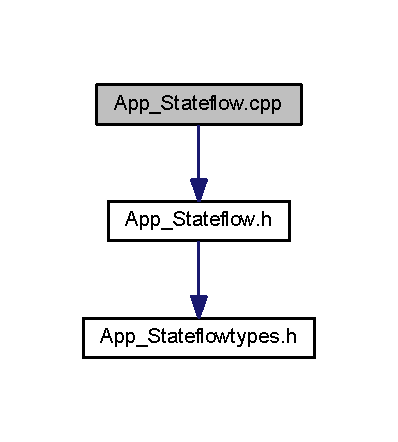
\includegraphics[width=191pt]{_app___stateflow_8cpp__incl}
\end{center}
\end{figure}
\subsection*{Macros}
\begin{DoxyCompactItemize}
\item 
\#define \mbox{\hyperlink{_app___stateflow_8cpp_aa817b31a7c7a0579da90fc2f2f15d222}{I\+N\+\_\+\+Backward}}~((\mbox{\hyperlink{_app___stateflowtypes_8h_a2532a6244e023eee49f315c10f1f7c53}{uint8\+\_\+T}})1\+U)
\item 
\#define \mbox{\hyperlink{_app___stateflow_8cpp_a10740620ab078458692c597c5e13d505}{I\+N\+\_\+\+Forward}}~((\mbox{\hyperlink{_app___stateflowtypes_8h_a2532a6244e023eee49f315c10f1f7c53}{uint8\+\_\+T}})2\+U)
\item 
\#define \mbox{\hyperlink{_app___stateflow_8cpp_ad477d4e95ca49acd2ca68907748c4abb}{I\+N\+\_\+\+Idle}}~((\mbox{\hyperlink{_app___stateflowtypes_8h_a2532a6244e023eee49f315c10f1f7c53}{uint8\+\_\+T}})3\+U)
\item 
\#define \mbox{\hyperlink{_app___stateflow_8cpp_a2030f1fd23aa500421f2ce7b71cdcf65}{I\+N\+\_\+\+Turn\+\_\+\+Left}}~((\mbox{\hyperlink{_app___stateflowtypes_8h_a2532a6244e023eee49f315c10f1f7c53}{uint8\+\_\+T}})4\+U)
\item 
\#define \mbox{\hyperlink{_app___stateflow_8cpp_a512c2b4d6d5dc6895929ea57a8b066ba}{I\+N\+\_\+\+Turn\+\_\+\+Right}}~((\mbox{\hyperlink{_app___stateflowtypes_8h_a2532a6244e023eee49f315c10f1f7c53}{uint8\+\_\+T}})5\+U)
\end{DoxyCompactItemize}


\subsection{Detailed Description}
Application file for Stateflow. 

\begin{DoxyAuthor}{Author}
Hannes Bähr, Juliane Müller 
\end{DoxyAuthor}
\begin{DoxyDate}{Date}
January 31, 2019 
\end{DoxyDate}
\hypertarget{_app___stateflowtypes_8h_Code_generation}{}\subsection{code\+\_\+generation}\label{_app___stateflowtypes_8h_Code_generation}
Code generated for Simulink model \textquotesingle{}Chart\textquotesingle{}. Model version \+: 1.\+40 Simulink Coder version \+: 8.\+14 (R2018a) 06-\/\+Feb-\/2018 C/\+C++ source code generated on \+: Thu Jan 24 11\+:08\+:26 2018 Embedded hardware selection\+: Atmel-\/$>$A\+VR (8-\/bit) 

\subsection{Macro Definition Documentation}
\mbox{\Hypertarget{_app___stateflow_8cpp_aa817b31a7c7a0579da90fc2f2f15d222}\label{_app___stateflow_8cpp_aa817b31a7c7a0579da90fc2f2f15d222}} 
\index{App\+\_\+\+Stateflow.\+cpp@{App\+\_\+\+Stateflow.\+cpp}!I\+N\+\_\+\+Backward@{I\+N\+\_\+\+Backward}}
\index{I\+N\+\_\+\+Backward@{I\+N\+\_\+\+Backward}!App\+\_\+\+Stateflow.\+cpp@{App\+\_\+\+Stateflow.\+cpp}}
\subsubsection{\texorpdfstring{I\+N\+\_\+\+Backward}{IN\_Backward}}
{\footnotesize\ttfamily \#define I\+N\+\_\+\+Backward~((\mbox{\hyperlink{_app___stateflowtypes_8h_a2532a6244e023eee49f315c10f1f7c53}{uint8\+\_\+T}})1\+U)}



Definition at line 22 of file App\+\_\+\+Stateflow.\+cpp.

\mbox{\Hypertarget{_app___stateflow_8cpp_a10740620ab078458692c597c5e13d505}\label{_app___stateflow_8cpp_a10740620ab078458692c597c5e13d505}} 
\index{App\+\_\+\+Stateflow.\+cpp@{App\+\_\+\+Stateflow.\+cpp}!I\+N\+\_\+\+Forward@{I\+N\+\_\+\+Forward}}
\index{I\+N\+\_\+\+Forward@{I\+N\+\_\+\+Forward}!App\+\_\+\+Stateflow.\+cpp@{App\+\_\+\+Stateflow.\+cpp}}
\subsubsection{\texorpdfstring{I\+N\+\_\+\+Forward}{IN\_Forward}}
{\footnotesize\ttfamily \#define I\+N\+\_\+\+Forward~((\mbox{\hyperlink{_app___stateflowtypes_8h_a2532a6244e023eee49f315c10f1f7c53}{uint8\+\_\+T}})2\+U)}



Definition at line 23 of file App\+\_\+\+Stateflow.\+cpp.

\mbox{\Hypertarget{_app___stateflow_8cpp_ad477d4e95ca49acd2ca68907748c4abb}\label{_app___stateflow_8cpp_ad477d4e95ca49acd2ca68907748c4abb}} 
\index{App\+\_\+\+Stateflow.\+cpp@{App\+\_\+\+Stateflow.\+cpp}!I\+N\+\_\+\+Idle@{I\+N\+\_\+\+Idle}}
\index{I\+N\+\_\+\+Idle@{I\+N\+\_\+\+Idle}!App\+\_\+\+Stateflow.\+cpp@{App\+\_\+\+Stateflow.\+cpp}}
\subsubsection{\texorpdfstring{I\+N\+\_\+\+Idle}{IN\_Idle}}
{\footnotesize\ttfamily \#define I\+N\+\_\+\+Idle~((\mbox{\hyperlink{_app___stateflowtypes_8h_a2532a6244e023eee49f315c10f1f7c53}{uint8\+\_\+T}})3\+U)}



Definition at line 24 of file App\+\_\+\+Stateflow.\+cpp.

\mbox{\Hypertarget{_app___stateflow_8cpp_a2030f1fd23aa500421f2ce7b71cdcf65}\label{_app___stateflow_8cpp_a2030f1fd23aa500421f2ce7b71cdcf65}} 
\index{App\+\_\+\+Stateflow.\+cpp@{App\+\_\+\+Stateflow.\+cpp}!I\+N\+\_\+\+Turn\+\_\+\+Left@{I\+N\+\_\+\+Turn\+\_\+\+Left}}
\index{I\+N\+\_\+\+Turn\+\_\+\+Left@{I\+N\+\_\+\+Turn\+\_\+\+Left}!App\+\_\+\+Stateflow.\+cpp@{App\+\_\+\+Stateflow.\+cpp}}
\subsubsection{\texorpdfstring{I\+N\+\_\+\+Turn\+\_\+\+Left}{IN\_Turn\_Left}}
{\footnotesize\ttfamily \#define I\+N\+\_\+\+Turn\+\_\+\+Left~((\mbox{\hyperlink{_app___stateflowtypes_8h_a2532a6244e023eee49f315c10f1f7c53}{uint8\+\_\+T}})4\+U)}



Definition at line 25 of file App\+\_\+\+Stateflow.\+cpp.

\mbox{\Hypertarget{_app___stateflow_8cpp_a512c2b4d6d5dc6895929ea57a8b066ba}\label{_app___stateflow_8cpp_a512c2b4d6d5dc6895929ea57a8b066ba}} 
\index{App\+\_\+\+Stateflow.\+cpp@{App\+\_\+\+Stateflow.\+cpp}!I\+N\+\_\+\+Turn\+\_\+\+Right@{I\+N\+\_\+\+Turn\+\_\+\+Right}}
\index{I\+N\+\_\+\+Turn\+\_\+\+Right@{I\+N\+\_\+\+Turn\+\_\+\+Right}!App\+\_\+\+Stateflow.\+cpp@{App\+\_\+\+Stateflow.\+cpp}}
\subsubsection{\texorpdfstring{I\+N\+\_\+\+Turn\+\_\+\+Right}{IN\_Turn\_Right}}
{\footnotesize\ttfamily \#define I\+N\+\_\+\+Turn\+\_\+\+Right~((\mbox{\hyperlink{_app___stateflowtypes_8h_a2532a6244e023eee49f315c10f1f7c53}{uint8\+\_\+T}})5\+U)}



Definition at line 26 of file App\+\_\+\+Stateflow.\+cpp.


\hypertarget{_app___stateflow_8h}{}\section{App\+\_\+\+Stateflow.\+h File Reference}
\label{_app___stateflow_8h}\index{App\+\_\+\+Stateflow.\+h@{App\+\_\+\+Stateflow.\+h}}


Application file for Stateflow.  


{\ttfamily \#include \char`\"{}App\+\_\+\+Stateflowtypes.\+h\char`\"{}}\newline
Include dependency graph for App\+\_\+\+Stateflow.\+h\+:
\nopagebreak
\begin{figure}[H]
\begin{center}
\leavevmode
\includegraphics[width=191pt]{_app___stateflow_8h__incl}
\end{center}
\end{figure}
This graph shows which files directly or indirectly include this file\+:
\nopagebreak
\begin{figure}[H]
\begin{center}
\leavevmode
\includegraphics[width=350pt]{_app___stateflow_8h__dep__incl}
\end{center}
\end{figure}
\subsection*{Classes}
\begin{DoxyCompactItemize}
\item 
struct \mbox{\hyperlink{struct_d_w}{DW}}
\begin{DoxyCompactList}\small\item\em Local signals for Stateflow. \end{DoxyCompactList}\item 
struct \mbox{\hyperlink{struct_ext_u}{ExtU}}
\begin{DoxyCompactList}\small\item\em External inputs for Stateflow. \end{DoxyCompactList}\item 
struct \mbox{\hyperlink{struct_ext_y}{ExtY}}
\begin{DoxyCompactList}\small\item\em External outputs for Stateflow. \end{DoxyCompactList}\item 
struct \mbox{\hyperlink{structtag___r_t_m}{tag\+\_\+\+R\+TM}}
\begin{DoxyCompactList}\small\item\em Forward declaration for rt\+Model. \end{DoxyCompactList}\item 
class \mbox{\hyperlink{class_chart_model_class}{Chart\+Model\+Class}}
\begin{DoxyCompactList}\small\item\em Class declaration of the chart model. \end{DoxyCompactList}\end{DoxyCompactItemize}
\subsection*{Macros}
\begin{DoxyCompactItemize}
\item 
\#define \mbox{\hyperlink{_app___stateflow_8h_a124ad07e78ce88e087803a80c5fd00aa}{Chart\+\_\+\+C\+O\+M\+M\+O\+N\+\_\+\+I\+N\+C\+L\+U\+D\+E\+S\+\_\+}}
\item 
\#define \mbox{\hyperlink{_app___stateflow_8h_a557d264325c9e243515f06d77552c662}{rtm\+Get\+Error\+Status}}(rtm)~((rtm)-\/$>$error\+Status)
\item 
\#define \mbox{\hyperlink{_app___stateflow_8h_a068bf11f899627a85b3c169391608c78}{rtm\+Set\+Error\+Status}}(rtm,  val)~((rtm)-\/$>$error\+Status = (val))
\end{DoxyCompactItemize}
\subsection*{Typedefs}
\begin{DoxyCompactItemize}
\item 
typedef struct \mbox{\hyperlink{structtag___r_t_m}{tag\+\_\+\+R\+TM}} \mbox{\hyperlink{_app___stateflow_8h_a6f32dbbab0d15102b3fe6ec3fe6a72ba}{R\+T\+\_\+\+M\+O\+D\+EL}}
\end{DoxyCompactItemize}


\subsection{Detailed Description}
Application file for Stateflow. 

\begin{DoxyAuthor}{Author}
Hannes Bähr, Juliane Müller 
\end{DoxyAuthor}
\begin{DoxyDate}{Date}
January 31, 2019 
\end{DoxyDate}
\hypertarget{_app___stateflowtypes_8h_Code_generation}{}\subsection{code\+\_\+generation}\label{_app___stateflowtypes_8h_Code_generation}
Code generated for Simulink model \textquotesingle{}Chart\textquotesingle{}. Model version \+: 1.\+37 Simulink Coder version \+: 8.\+14 (R2018a) 06-\/\+Feb-\/2018 C/\+C++ source code generated on \+: Mon Dec 10 09\+:08\+:26 2018 Embedded hardware selection\+: Atmel-\/$>$A\+VR (8-\/bit) 

\subsection{Macro Definition Documentation}
\mbox{\Hypertarget{_app___stateflow_8h_a124ad07e78ce88e087803a80c5fd00aa}\label{_app___stateflow_8h_a124ad07e78ce88e087803a80c5fd00aa}} 
\index{App\+\_\+\+Stateflow.\+h@{App\+\_\+\+Stateflow.\+h}!Chart\+\_\+\+C\+O\+M\+M\+O\+N\+\_\+\+I\+N\+C\+L\+U\+D\+E\+S\+\_\+@{Chart\+\_\+\+C\+O\+M\+M\+O\+N\+\_\+\+I\+N\+C\+L\+U\+D\+E\+S\+\_\+}}
\index{Chart\+\_\+\+C\+O\+M\+M\+O\+N\+\_\+\+I\+N\+C\+L\+U\+D\+E\+S\+\_\+@{Chart\+\_\+\+C\+O\+M\+M\+O\+N\+\_\+\+I\+N\+C\+L\+U\+D\+E\+S\+\_\+}!App\+\_\+\+Stateflow.\+h@{App\+\_\+\+Stateflow.\+h}}
\subsubsection{\texorpdfstring{Chart\+\_\+\+C\+O\+M\+M\+O\+N\+\_\+\+I\+N\+C\+L\+U\+D\+E\+S\+\_\+}{Chart\_COMMON\_INCLUDES\_}}
{\footnotesize\ttfamily \#define Chart\+\_\+\+C\+O\+M\+M\+O\+N\+\_\+\+I\+N\+C\+L\+U\+D\+E\+S\+\_\+}



Definition at line 23 of file App\+\_\+\+Stateflow.\+h.

\mbox{\Hypertarget{_app___stateflow_8h_a557d264325c9e243515f06d77552c662}\label{_app___stateflow_8h_a557d264325c9e243515f06d77552c662}} 
\index{App\+\_\+\+Stateflow.\+h@{App\+\_\+\+Stateflow.\+h}!rtm\+Get\+Error\+Status@{rtm\+Get\+Error\+Status}}
\index{rtm\+Get\+Error\+Status@{rtm\+Get\+Error\+Status}!App\+\_\+\+Stateflow.\+h@{App\+\_\+\+Stateflow.\+h}}
\subsubsection{\texorpdfstring{rtm\+Get\+Error\+Status}{rtmGetErrorStatus}}
{\footnotesize\ttfamily \#define rtm\+Get\+Error\+Status(\begin{DoxyParamCaption}\item[{}]{rtm }\end{DoxyParamCaption})~((rtm)-\/$>$error\+Status)}



Definition at line 27 of file App\+\_\+\+Stateflow.\+h.

\mbox{\Hypertarget{_app___stateflow_8h_a068bf11f899627a85b3c169391608c78}\label{_app___stateflow_8h_a068bf11f899627a85b3c169391608c78}} 
\index{App\+\_\+\+Stateflow.\+h@{App\+\_\+\+Stateflow.\+h}!rtm\+Set\+Error\+Status@{rtm\+Set\+Error\+Status}}
\index{rtm\+Set\+Error\+Status@{rtm\+Set\+Error\+Status}!App\+\_\+\+Stateflow.\+h@{App\+\_\+\+Stateflow.\+h}}
\subsubsection{\texorpdfstring{rtm\+Set\+Error\+Status}{rtmSetErrorStatus}}
{\footnotesize\ttfamily \#define rtm\+Set\+Error\+Status(\begin{DoxyParamCaption}\item[{}]{rtm,  }\item[{}]{val }\end{DoxyParamCaption})~((rtm)-\/$>$error\+Status = (val))}



Definition at line 31 of file App\+\_\+\+Stateflow.\+h.



\subsection{Typedef Documentation}
\mbox{\Hypertarget{_app___stateflow_8h_a6f32dbbab0d15102b3fe6ec3fe6a72ba}\label{_app___stateflow_8h_a6f32dbbab0d15102b3fe6ec3fe6a72ba}} 
\index{App\+\_\+\+Stateflow.\+h@{App\+\_\+\+Stateflow.\+h}!R\+T\+\_\+\+M\+O\+D\+EL@{R\+T\+\_\+\+M\+O\+D\+EL}}
\index{R\+T\+\_\+\+M\+O\+D\+EL@{R\+T\+\_\+\+M\+O\+D\+EL}!App\+\_\+\+Stateflow.\+h@{App\+\_\+\+Stateflow.\+h}}
\subsubsection{\texorpdfstring{R\+T\+\_\+\+M\+O\+D\+EL}{RT\_MODEL}}
{\footnotesize\ttfamily typedef struct \mbox{\hyperlink{structtag___r_t_m}{tag\+\_\+\+R\+TM}} \mbox{\hyperlink{_app___stateflow_8h_a6f32dbbab0d15102b3fe6ec3fe6a72ba}{R\+T\+\_\+\+M\+O\+D\+EL}}}



Definition at line 47 of file App\+\_\+\+Stateflow.\+h.


\hypertarget{_app___stateflowtypes_8h}{}\section{App\+\_\+\+Stateflowtypes.\+h File Reference}
\label{_app___stateflowtypes_8h}\index{App\+\_\+\+Stateflowtypes.\+h@{App\+\_\+\+Stateflowtypes.\+h}}


Application file for Stateflowtypes.  


This graph shows which files directly or indirectly include this file\+:
\nopagebreak
\begin{figure}[H]
\begin{center}
\leavevmode
\includegraphics[width=350pt]{_app___stateflowtypes_8h__dep__incl}
\end{center}
\end{figure}
\subsection*{Macros}
\begin{DoxyCompactItemize}
\item 
\#define \mbox{\hyperlink{_app___stateflowtypes_8h_a65e9886d74aaee76545e83dd09011727}{false}}~(0\+U)
\item 
\#define \mbox{\hyperlink{_app___stateflowtypes_8h_a41f9c5fb8b08eb5dc3edce4dcb37fee7}{true}}~(1\+U)
\item 
\#define \mbox{\hyperlink{_app___stateflowtypes_8h_afc0fac7fa072abb8fc3da29d89a5a250}{M\+A\+X\+\_\+int8\+\_\+T}}~((\mbox{\hyperlink{_app___stateflowtypes_8h_ab7f14b954bf92a066b5a5cbc6f28b349}{int8\+\_\+T}})(127))
\item 
\#define \mbox{\hyperlink{_app___stateflowtypes_8h_af171ef95a0a296c4a6191c4fa9a6b188}{M\+I\+N\+\_\+int8\+\_\+T}}~((\mbox{\hyperlink{_app___stateflowtypes_8h_ab7f14b954bf92a066b5a5cbc6f28b349}{int8\+\_\+T}})(-\/128))
\item 
\#define \mbox{\hyperlink{_app___stateflowtypes_8h_a8041c00ac8c3fa3586faec62da663985}{M\+A\+X\+\_\+uint8\+\_\+T}}~((\mbox{\hyperlink{_app___stateflowtypes_8h_a2532a6244e023eee49f315c10f1f7c53}{uint8\+\_\+T}})(255\+U))
\item 
\#define \mbox{\hyperlink{_app___stateflowtypes_8h_a2aa4d5510e52efd157ad1cd2c7635b48}{M\+A\+X\+\_\+int16\+\_\+T}}~((\mbox{\hyperlink{_app___stateflowtypes_8h_ad73c6af88bb2ce70799e51f639309f21}{int16\+\_\+T}})(32767))
\item 
\#define \mbox{\hyperlink{_app___stateflowtypes_8h_a6af1fb7c9084add0122589e8578f00ce}{M\+I\+N\+\_\+int16\+\_\+T}}~((\mbox{\hyperlink{_app___stateflowtypes_8h_ad73c6af88bb2ce70799e51f639309f21}{int16\+\_\+T}})(-\/32768))
\item 
\#define \mbox{\hyperlink{_app___stateflowtypes_8h_a5f69d019adce227ecfb104b7139aa52a}{M\+A\+X\+\_\+uint16\+\_\+T}}~((\mbox{\hyperlink{_app___stateflowtypes_8h_ab04e0d1bcae39d77ad28252ab0eb90a4}{uint16\+\_\+T}})(65535\+U))
\item 
\#define \mbox{\hyperlink{_app___stateflowtypes_8h_a4e3b5c01e2881b076e36c72b5966cb55}{M\+A\+X\+\_\+int32\+\_\+T}}~((\mbox{\hyperlink{_app___stateflowtypes_8h_ae5c7906acb8ff3e26c787c3e3ed99142}{int32\+\_\+T}})(2147483647\+L))
\item 
\#define \mbox{\hyperlink{_app___stateflowtypes_8h_a1991e25fc2c03e1bf55b4abe570317bd}{M\+I\+N\+\_\+int32\+\_\+T}}~((\mbox{\hyperlink{_app___stateflowtypes_8h_ae5c7906acb8ff3e26c787c3e3ed99142}{int32\+\_\+T}})(-\/2147483647\+L-\/1\+L))
\item 
\#define \mbox{\hyperlink{_app___stateflowtypes_8h_af3b12d911332c30bc150743e1196660a}{M\+A\+X\+\_\+uint32\+\_\+T}}~((\mbox{\hyperlink{_app___stateflowtypes_8h_a7af70b427480b10d9ea56c51693a061f}{uint32\+\_\+T}})(0x\+F\+F\+F\+F\+F\+F\+F\+F\+U\+L))
\item 
\#define \mbox{\hyperlink{_app___stateflowtypes_8h_a759f49acee7719764fe27eb92de3dca0}{M\+A\+X\+\_\+int64\+\_\+T}}~((\mbox{\hyperlink{_app___stateflowtypes_8h_a9f80a0238d372731ee0bed805f228dd1}{int64\+\_\+T}})(9223372036854775807\+L\+L))
\item 
\#define \mbox{\hyperlink{_app___stateflowtypes_8h_afa7f5d4e259dc11a355c432ee7605b1c}{M\+I\+N\+\_\+int64\+\_\+T}}~((\mbox{\hyperlink{_app___stateflowtypes_8h_a9f80a0238d372731ee0bed805f228dd1}{int64\+\_\+T}})(-\/9223372036854775807\+L\+L-\/1\+L\+L))
\item 
\#define \mbox{\hyperlink{_app___stateflowtypes_8h_ab4e249675db6a13f72914d4a0ca36364}{M\+A\+X\+\_\+uint64\+\_\+T}}~((\mbox{\hyperlink{_app___stateflowtypes_8h_a20576136ba7f730cbedb691373c09663}{uint64\+\_\+T}})(0x\+F\+F\+F\+F\+F\+F\+F\+F\+F\+F\+F\+F\+F\+F\+F\+F\+U\+L\+L))
\end{DoxyCompactItemize}
\subsection*{Typedefs}
\begin{DoxyCompactItemize}
\item 
typedef signed char \mbox{\hyperlink{_app___stateflowtypes_8h_ab7f14b954bf92a066b5a5cbc6f28b349}{int8\+\_\+T}}
\item 
typedef unsigned char \mbox{\hyperlink{_app___stateflowtypes_8h_a2532a6244e023eee49f315c10f1f7c53}{uint8\+\_\+T}}
\item 
typedef int \mbox{\hyperlink{_app___stateflowtypes_8h_ad73c6af88bb2ce70799e51f639309f21}{int16\+\_\+T}}
\item 
typedef unsigned int \mbox{\hyperlink{_app___stateflowtypes_8h_ab04e0d1bcae39d77ad28252ab0eb90a4}{uint16\+\_\+T}}
\item 
typedef long \mbox{\hyperlink{_app___stateflowtypes_8h_ae5c7906acb8ff3e26c787c3e3ed99142}{int32\+\_\+T}}
\item 
typedef unsigned long \mbox{\hyperlink{_app___stateflowtypes_8h_a7af70b427480b10d9ea56c51693a061f}{uint32\+\_\+T}}
\item 
typedef long long \mbox{\hyperlink{_app___stateflowtypes_8h_a9f80a0238d372731ee0bed805f228dd1}{int64\+\_\+T}}
\item 
typedef unsigned long long \mbox{\hyperlink{_app___stateflowtypes_8h_a20576136ba7f730cbedb691373c09663}{uint64\+\_\+T}}
\item 
typedef unsigned char \mbox{\hyperlink{_app___stateflowtypes_8h_a3f14692b9a04d8211058e2bfc777a9fc}{boolean\+\_\+T}}
\item 
typedef int \mbox{\hyperlink{_app___stateflowtypes_8h_a708854ed500d1aada8fa33d38ed54fbf}{int\+\_\+T}}
\item 
typedef unsigned int \mbox{\hyperlink{_app___stateflowtypes_8h_a812dbe96020cf6b5c4a14e9339fc0d11}{uint\+\_\+T}}
\item 
typedef unsigned long \mbox{\hyperlink{_app___stateflowtypes_8h_a990999404045826a6e03f9b7d89bdf0e}{ulong\+\_\+T}}
\item 
typedef unsigned long long \mbox{\hyperlink{_app___stateflowtypes_8h_a875098f46f2dfed9281375dde6b70e06}{ulonglong\+\_\+T}}
\item 
typedef char \mbox{\hyperlink{_app___stateflowtypes_8h_a0fd897430c65dad7d2638a12bc4ea8b5}{char\+\_\+T}}
\item 
typedef unsigned char \mbox{\hyperlink{_app___stateflowtypes_8h_a2a3d79bdfc1d71f98235f70e68914302}{uchar\+\_\+T}}
\item 
typedef \mbox{\hyperlink{_app___stateflowtypes_8h_a0fd897430c65dad7d2638a12bc4ea8b5}{char\+\_\+T}} \mbox{\hyperlink{_app___stateflowtypes_8h_a803796e8caccf808b38c550adf62f400}{byte\+\_\+T}}
\item 
typedef void $\ast$ \mbox{\hyperlink{_app___stateflowtypes_8h_a9d78476406d2c523314d98d694659251}{pointer\+\_\+T}}
\end{DoxyCompactItemize}


\subsection{Detailed Description}
Application file for Stateflowtypes. 

\begin{DoxyAuthor}{Author}
Hannes Bähr, Juliane Müller 
\end{DoxyAuthor}
\begin{DoxyDate}{Date}
January 31, 2019 
\end{DoxyDate}
\hypertarget{_app___stateflowtypes_8h_Code_generation}{}\subsection{code\+\_\+generation}\label{_app___stateflowtypes_8h_Code_generation}
Code generated for Simulink model \textquotesingle{}Chart\textquotesingle{}. Model version \+: 1.\+37 Simulink Coder version \+: 8.\+14 (R2018a) 06-\/\+Feb-\/2018 C/\+C++ source code generated on \+: Mon Dec 10 09\+:08\+:26 2018 Embedded hardware selection\+: Atmel-\/$>$A\+VR (8-\/bit) 

\subsection{Macro Definition Documentation}
\mbox{\Hypertarget{_app___stateflowtypes_8h_a65e9886d74aaee76545e83dd09011727}\label{_app___stateflowtypes_8h_a65e9886d74aaee76545e83dd09011727}} 
\index{App\+\_\+\+Stateflowtypes.\+h@{App\+\_\+\+Stateflowtypes.\+h}!false@{false}}
\index{false@{false}!App\+\_\+\+Stateflowtypes.\+h@{App\+\_\+\+Stateflowtypes.\+h}}
\subsubsection{\texorpdfstring{false}{false}}
{\footnotesize\ttfamily \#define false~(0\+U)}



Definition at line 26 of file App\+\_\+\+Stateflowtypes.\+h.

\mbox{\Hypertarget{_app___stateflowtypes_8h_a2aa4d5510e52efd157ad1cd2c7635b48}\label{_app___stateflowtypes_8h_a2aa4d5510e52efd157ad1cd2c7635b48}} 
\index{App\+\_\+\+Stateflowtypes.\+h@{App\+\_\+\+Stateflowtypes.\+h}!M\+A\+X\+\_\+int16\+\_\+T@{M\+A\+X\+\_\+int16\+\_\+T}}
\index{M\+A\+X\+\_\+int16\+\_\+T@{M\+A\+X\+\_\+int16\+\_\+T}!App\+\_\+\+Stateflowtypes.\+h@{App\+\_\+\+Stateflowtypes.\+h}}
\subsubsection{\texorpdfstring{M\+A\+X\+\_\+int16\+\_\+T}{MAX\_int16\_T}}
{\footnotesize\ttfamily \#define M\+A\+X\+\_\+int16\+\_\+T~((\mbox{\hyperlink{_app___stateflowtypes_8h_ad73c6af88bb2ce70799e51f639309f21}{int16\+\_\+T}})(32767))}



Definition at line 80 of file App\+\_\+\+Stateflowtypes.\+h.

\mbox{\Hypertarget{_app___stateflowtypes_8h_a4e3b5c01e2881b076e36c72b5966cb55}\label{_app___stateflowtypes_8h_a4e3b5c01e2881b076e36c72b5966cb55}} 
\index{App\+\_\+\+Stateflowtypes.\+h@{App\+\_\+\+Stateflowtypes.\+h}!M\+A\+X\+\_\+int32\+\_\+T@{M\+A\+X\+\_\+int32\+\_\+T}}
\index{M\+A\+X\+\_\+int32\+\_\+T@{M\+A\+X\+\_\+int32\+\_\+T}!App\+\_\+\+Stateflowtypes.\+h@{App\+\_\+\+Stateflowtypes.\+h}}
\subsubsection{\texorpdfstring{M\+A\+X\+\_\+int32\+\_\+T}{MAX\_int32\_T}}
{\footnotesize\ttfamily \#define M\+A\+X\+\_\+int32\+\_\+T~((\mbox{\hyperlink{_app___stateflowtypes_8h_ae5c7906acb8ff3e26c787c3e3ed99142}{int32\+\_\+T}})(2147483647\+L))}



Definition at line 83 of file App\+\_\+\+Stateflowtypes.\+h.

\mbox{\Hypertarget{_app___stateflowtypes_8h_a759f49acee7719764fe27eb92de3dca0}\label{_app___stateflowtypes_8h_a759f49acee7719764fe27eb92de3dca0}} 
\index{App\+\_\+\+Stateflowtypes.\+h@{App\+\_\+\+Stateflowtypes.\+h}!M\+A\+X\+\_\+int64\+\_\+T@{M\+A\+X\+\_\+int64\+\_\+T}}
\index{M\+A\+X\+\_\+int64\+\_\+T@{M\+A\+X\+\_\+int64\+\_\+T}!App\+\_\+\+Stateflowtypes.\+h@{App\+\_\+\+Stateflowtypes.\+h}}
\subsubsection{\texorpdfstring{M\+A\+X\+\_\+int64\+\_\+T}{MAX\_int64\_T}}
{\footnotesize\ttfamily \#define M\+A\+X\+\_\+int64\+\_\+T~((\mbox{\hyperlink{_app___stateflowtypes_8h_a9f80a0238d372731ee0bed805f228dd1}{int64\+\_\+T}})(9223372036854775807\+L\+L))}



Definition at line 86 of file App\+\_\+\+Stateflowtypes.\+h.

\mbox{\Hypertarget{_app___stateflowtypes_8h_afc0fac7fa072abb8fc3da29d89a5a250}\label{_app___stateflowtypes_8h_afc0fac7fa072abb8fc3da29d89a5a250}} 
\index{App\+\_\+\+Stateflowtypes.\+h@{App\+\_\+\+Stateflowtypes.\+h}!M\+A\+X\+\_\+int8\+\_\+T@{M\+A\+X\+\_\+int8\+\_\+T}}
\index{M\+A\+X\+\_\+int8\+\_\+T@{M\+A\+X\+\_\+int8\+\_\+T}!App\+\_\+\+Stateflowtypes.\+h@{App\+\_\+\+Stateflowtypes.\+h}}
\subsubsection{\texorpdfstring{M\+A\+X\+\_\+int8\+\_\+T}{MAX\_int8\_T}}
{\footnotesize\ttfamily \#define M\+A\+X\+\_\+int8\+\_\+T~((\mbox{\hyperlink{_app___stateflowtypes_8h_ab7f14b954bf92a066b5a5cbc6f28b349}{int8\+\_\+T}})(127))}



Definition at line 77 of file App\+\_\+\+Stateflowtypes.\+h.

\mbox{\Hypertarget{_app___stateflowtypes_8h_a5f69d019adce227ecfb104b7139aa52a}\label{_app___stateflowtypes_8h_a5f69d019adce227ecfb104b7139aa52a}} 
\index{App\+\_\+\+Stateflowtypes.\+h@{App\+\_\+\+Stateflowtypes.\+h}!M\+A\+X\+\_\+uint16\+\_\+T@{M\+A\+X\+\_\+uint16\+\_\+T}}
\index{M\+A\+X\+\_\+uint16\+\_\+T@{M\+A\+X\+\_\+uint16\+\_\+T}!App\+\_\+\+Stateflowtypes.\+h@{App\+\_\+\+Stateflowtypes.\+h}}
\subsubsection{\texorpdfstring{M\+A\+X\+\_\+uint16\+\_\+T}{MAX\_uint16\_T}}
{\footnotesize\ttfamily \#define M\+A\+X\+\_\+uint16\+\_\+T~((\mbox{\hyperlink{_app___stateflowtypes_8h_ab04e0d1bcae39d77ad28252ab0eb90a4}{uint16\+\_\+T}})(65535\+U))}



Definition at line 82 of file App\+\_\+\+Stateflowtypes.\+h.

\mbox{\Hypertarget{_app___stateflowtypes_8h_af3b12d911332c30bc150743e1196660a}\label{_app___stateflowtypes_8h_af3b12d911332c30bc150743e1196660a}} 
\index{App\+\_\+\+Stateflowtypes.\+h@{App\+\_\+\+Stateflowtypes.\+h}!M\+A\+X\+\_\+uint32\+\_\+T@{M\+A\+X\+\_\+uint32\+\_\+T}}
\index{M\+A\+X\+\_\+uint32\+\_\+T@{M\+A\+X\+\_\+uint32\+\_\+T}!App\+\_\+\+Stateflowtypes.\+h@{App\+\_\+\+Stateflowtypes.\+h}}
\subsubsection{\texorpdfstring{M\+A\+X\+\_\+uint32\+\_\+T}{MAX\_uint32\_T}}
{\footnotesize\ttfamily \#define M\+A\+X\+\_\+uint32\+\_\+T~((\mbox{\hyperlink{_app___stateflowtypes_8h_a7af70b427480b10d9ea56c51693a061f}{uint32\+\_\+T}})(0x\+F\+F\+F\+F\+F\+F\+F\+F\+U\+L))}



Definition at line 85 of file App\+\_\+\+Stateflowtypes.\+h.

\mbox{\Hypertarget{_app___stateflowtypes_8h_ab4e249675db6a13f72914d4a0ca36364}\label{_app___stateflowtypes_8h_ab4e249675db6a13f72914d4a0ca36364}} 
\index{App\+\_\+\+Stateflowtypes.\+h@{App\+\_\+\+Stateflowtypes.\+h}!M\+A\+X\+\_\+uint64\+\_\+T@{M\+A\+X\+\_\+uint64\+\_\+T}}
\index{M\+A\+X\+\_\+uint64\+\_\+T@{M\+A\+X\+\_\+uint64\+\_\+T}!App\+\_\+\+Stateflowtypes.\+h@{App\+\_\+\+Stateflowtypes.\+h}}
\subsubsection{\texorpdfstring{M\+A\+X\+\_\+uint64\+\_\+T}{MAX\_uint64\_T}}
{\footnotesize\ttfamily \#define M\+A\+X\+\_\+uint64\+\_\+T~((\mbox{\hyperlink{_app___stateflowtypes_8h_a20576136ba7f730cbedb691373c09663}{uint64\+\_\+T}})(0x\+F\+F\+F\+F\+F\+F\+F\+F\+F\+F\+F\+F\+F\+F\+F\+F\+U\+L\+L))}



Definition at line 88 of file App\+\_\+\+Stateflowtypes.\+h.

\mbox{\Hypertarget{_app___stateflowtypes_8h_a8041c00ac8c3fa3586faec62da663985}\label{_app___stateflowtypes_8h_a8041c00ac8c3fa3586faec62da663985}} 
\index{App\+\_\+\+Stateflowtypes.\+h@{App\+\_\+\+Stateflowtypes.\+h}!M\+A\+X\+\_\+uint8\+\_\+T@{M\+A\+X\+\_\+uint8\+\_\+T}}
\index{M\+A\+X\+\_\+uint8\+\_\+T@{M\+A\+X\+\_\+uint8\+\_\+T}!App\+\_\+\+Stateflowtypes.\+h@{App\+\_\+\+Stateflowtypes.\+h}}
\subsubsection{\texorpdfstring{M\+A\+X\+\_\+uint8\+\_\+T}{MAX\_uint8\_T}}
{\footnotesize\ttfamily \#define M\+A\+X\+\_\+uint8\+\_\+T~((\mbox{\hyperlink{_app___stateflowtypes_8h_a2532a6244e023eee49f315c10f1f7c53}{uint8\+\_\+T}})(255\+U))}



Definition at line 79 of file App\+\_\+\+Stateflowtypes.\+h.

\mbox{\Hypertarget{_app___stateflowtypes_8h_a6af1fb7c9084add0122589e8578f00ce}\label{_app___stateflowtypes_8h_a6af1fb7c9084add0122589e8578f00ce}} 
\index{App\+\_\+\+Stateflowtypes.\+h@{App\+\_\+\+Stateflowtypes.\+h}!M\+I\+N\+\_\+int16\+\_\+T@{M\+I\+N\+\_\+int16\+\_\+T}}
\index{M\+I\+N\+\_\+int16\+\_\+T@{M\+I\+N\+\_\+int16\+\_\+T}!App\+\_\+\+Stateflowtypes.\+h@{App\+\_\+\+Stateflowtypes.\+h}}
\subsubsection{\texorpdfstring{M\+I\+N\+\_\+int16\+\_\+T}{MIN\_int16\_T}}
{\footnotesize\ttfamily \#define M\+I\+N\+\_\+int16\+\_\+T~((\mbox{\hyperlink{_app___stateflowtypes_8h_ad73c6af88bb2ce70799e51f639309f21}{int16\+\_\+T}})(-\/32768))}



Definition at line 81 of file App\+\_\+\+Stateflowtypes.\+h.

\mbox{\Hypertarget{_app___stateflowtypes_8h_a1991e25fc2c03e1bf55b4abe570317bd}\label{_app___stateflowtypes_8h_a1991e25fc2c03e1bf55b4abe570317bd}} 
\index{App\+\_\+\+Stateflowtypes.\+h@{App\+\_\+\+Stateflowtypes.\+h}!M\+I\+N\+\_\+int32\+\_\+T@{M\+I\+N\+\_\+int32\+\_\+T}}
\index{M\+I\+N\+\_\+int32\+\_\+T@{M\+I\+N\+\_\+int32\+\_\+T}!App\+\_\+\+Stateflowtypes.\+h@{App\+\_\+\+Stateflowtypes.\+h}}
\subsubsection{\texorpdfstring{M\+I\+N\+\_\+int32\+\_\+T}{MIN\_int32\_T}}
{\footnotesize\ttfamily \#define M\+I\+N\+\_\+int32\+\_\+T~((\mbox{\hyperlink{_app___stateflowtypes_8h_ae5c7906acb8ff3e26c787c3e3ed99142}{int32\+\_\+T}})(-\/2147483647\+L-\/1\+L))}



Definition at line 84 of file App\+\_\+\+Stateflowtypes.\+h.

\mbox{\Hypertarget{_app___stateflowtypes_8h_afa7f5d4e259dc11a355c432ee7605b1c}\label{_app___stateflowtypes_8h_afa7f5d4e259dc11a355c432ee7605b1c}} 
\index{App\+\_\+\+Stateflowtypes.\+h@{App\+\_\+\+Stateflowtypes.\+h}!M\+I\+N\+\_\+int64\+\_\+T@{M\+I\+N\+\_\+int64\+\_\+T}}
\index{M\+I\+N\+\_\+int64\+\_\+T@{M\+I\+N\+\_\+int64\+\_\+T}!App\+\_\+\+Stateflowtypes.\+h@{App\+\_\+\+Stateflowtypes.\+h}}
\subsubsection{\texorpdfstring{M\+I\+N\+\_\+int64\+\_\+T}{MIN\_int64\_T}}
{\footnotesize\ttfamily \#define M\+I\+N\+\_\+int64\+\_\+T~((\mbox{\hyperlink{_app___stateflowtypes_8h_a9f80a0238d372731ee0bed805f228dd1}{int64\+\_\+T}})(-\/9223372036854775807\+L\+L-\/1\+L\+L))}



Definition at line 87 of file App\+\_\+\+Stateflowtypes.\+h.

\mbox{\Hypertarget{_app___stateflowtypes_8h_af171ef95a0a296c4a6191c4fa9a6b188}\label{_app___stateflowtypes_8h_af171ef95a0a296c4a6191c4fa9a6b188}} 
\index{App\+\_\+\+Stateflowtypes.\+h@{App\+\_\+\+Stateflowtypes.\+h}!M\+I\+N\+\_\+int8\+\_\+T@{M\+I\+N\+\_\+int8\+\_\+T}}
\index{M\+I\+N\+\_\+int8\+\_\+T@{M\+I\+N\+\_\+int8\+\_\+T}!App\+\_\+\+Stateflowtypes.\+h@{App\+\_\+\+Stateflowtypes.\+h}}
\subsubsection{\texorpdfstring{M\+I\+N\+\_\+int8\+\_\+T}{MIN\_int8\_T}}
{\footnotesize\ttfamily \#define M\+I\+N\+\_\+int8\+\_\+T~((\mbox{\hyperlink{_app___stateflowtypes_8h_ab7f14b954bf92a066b5a5cbc6f28b349}{int8\+\_\+T}})(-\/128))}



Definition at line 78 of file App\+\_\+\+Stateflowtypes.\+h.

\mbox{\Hypertarget{_app___stateflowtypes_8h_a41f9c5fb8b08eb5dc3edce4dcb37fee7}\label{_app___stateflowtypes_8h_a41f9c5fb8b08eb5dc3edce4dcb37fee7}} 
\index{App\+\_\+\+Stateflowtypes.\+h@{App\+\_\+\+Stateflowtypes.\+h}!true@{true}}
\index{true@{true}!App\+\_\+\+Stateflowtypes.\+h@{App\+\_\+\+Stateflowtypes.\+h}}
\subsubsection{\texorpdfstring{true}{true}}
{\footnotesize\ttfamily \#define true~(1\+U)}



Definition at line 30 of file App\+\_\+\+Stateflowtypes.\+h.



\subsection{Typedef Documentation}
\mbox{\Hypertarget{_app___stateflowtypes_8h_a3f14692b9a04d8211058e2bfc777a9fc}\label{_app___stateflowtypes_8h_a3f14692b9a04d8211058e2bfc777a9fc}} 
\index{App\+\_\+\+Stateflowtypes.\+h@{App\+\_\+\+Stateflowtypes.\+h}!boolean\+\_\+T@{boolean\+\_\+T}}
\index{boolean\+\_\+T@{boolean\+\_\+T}!App\+\_\+\+Stateflowtypes.\+h@{App\+\_\+\+Stateflowtypes.\+h}}
\subsubsection{\texorpdfstring{boolean\+\_\+T}{boolean\_T}}
{\footnotesize\ttfamily typedef unsigned char \mbox{\hyperlink{_app___stateflowtypes_8h_a3f14692b9a04d8211058e2bfc777a9fc}{boolean\+\_\+T}}}



Definition at line 63 of file App\+\_\+\+Stateflowtypes.\+h.

\mbox{\Hypertarget{_app___stateflowtypes_8h_a803796e8caccf808b38c550adf62f400}\label{_app___stateflowtypes_8h_a803796e8caccf808b38c550adf62f400}} 
\index{App\+\_\+\+Stateflowtypes.\+h@{App\+\_\+\+Stateflowtypes.\+h}!byte\+\_\+T@{byte\+\_\+T}}
\index{byte\+\_\+T@{byte\+\_\+T}!App\+\_\+\+Stateflowtypes.\+h@{App\+\_\+\+Stateflowtypes.\+h}}
\subsubsection{\texorpdfstring{byte\+\_\+T}{byte\_T}}
{\footnotesize\ttfamily typedef \mbox{\hyperlink{_app___stateflowtypes_8h_a0fd897430c65dad7d2638a12bc4ea8b5}{char\+\_\+T}} \mbox{\hyperlink{_app___stateflowtypes_8h_a803796e8caccf808b38c550adf62f400}{byte\+\_\+T}}}



Definition at line 70 of file App\+\_\+\+Stateflowtypes.\+h.

\mbox{\Hypertarget{_app___stateflowtypes_8h_a0fd897430c65dad7d2638a12bc4ea8b5}\label{_app___stateflowtypes_8h_a0fd897430c65dad7d2638a12bc4ea8b5}} 
\index{App\+\_\+\+Stateflowtypes.\+h@{App\+\_\+\+Stateflowtypes.\+h}!char\+\_\+T@{char\+\_\+T}}
\index{char\+\_\+T@{char\+\_\+T}!App\+\_\+\+Stateflowtypes.\+h@{App\+\_\+\+Stateflowtypes.\+h}}
\subsubsection{\texorpdfstring{char\+\_\+T}{char\_T}}
{\footnotesize\ttfamily typedef char \mbox{\hyperlink{_app___stateflowtypes_8h_a0fd897430c65dad7d2638a12bc4ea8b5}{char\+\_\+T}}}



Definition at line 68 of file App\+\_\+\+Stateflowtypes.\+h.

\mbox{\Hypertarget{_app___stateflowtypes_8h_ad73c6af88bb2ce70799e51f639309f21}\label{_app___stateflowtypes_8h_ad73c6af88bb2ce70799e51f639309f21}} 
\index{App\+\_\+\+Stateflowtypes.\+h@{App\+\_\+\+Stateflowtypes.\+h}!int16\+\_\+T@{int16\+\_\+T}}
\index{int16\+\_\+T@{int16\+\_\+T}!App\+\_\+\+Stateflowtypes.\+h@{App\+\_\+\+Stateflowtypes.\+h}}
\subsubsection{\texorpdfstring{int16\+\_\+T}{int16\_T}}
{\footnotesize\ttfamily typedef int \mbox{\hyperlink{_app___stateflowtypes_8h_ad73c6af88bb2ce70799e51f639309f21}{int16\+\_\+T}}}



Definition at line 52 of file App\+\_\+\+Stateflowtypes.\+h.

\mbox{\Hypertarget{_app___stateflowtypes_8h_ae5c7906acb8ff3e26c787c3e3ed99142}\label{_app___stateflowtypes_8h_ae5c7906acb8ff3e26c787c3e3ed99142}} 
\index{App\+\_\+\+Stateflowtypes.\+h@{App\+\_\+\+Stateflowtypes.\+h}!int32\+\_\+T@{int32\+\_\+T}}
\index{int32\+\_\+T@{int32\+\_\+T}!App\+\_\+\+Stateflowtypes.\+h@{App\+\_\+\+Stateflowtypes.\+h}}
\subsubsection{\texorpdfstring{int32\+\_\+T}{int32\_T}}
{\footnotesize\ttfamily typedef long \mbox{\hyperlink{_app___stateflowtypes_8h_ae5c7906acb8ff3e26c787c3e3ed99142}{int32\+\_\+T}}}



Definition at line 54 of file App\+\_\+\+Stateflowtypes.\+h.

\mbox{\Hypertarget{_app___stateflowtypes_8h_a9f80a0238d372731ee0bed805f228dd1}\label{_app___stateflowtypes_8h_a9f80a0238d372731ee0bed805f228dd1}} 
\index{App\+\_\+\+Stateflowtypes.\+h@{App\+\_\+\+Stateflowtypes.\+h}!int64\+\_\+T@{int64\+\_\+T}}
\index{int64\+\_\+T@{int64\+\_\+T}!App\+\_\+\+Stateflowtypes.\+h@{App\+\_\+\+Stateflowtypes.\+h}}
\subsubsection{\texorpdfstring{int64\+\_\+T}{int64\_T}}
{\footnotesize\ttfamily typedef long long \mbox{\hyperlink{_app___stateflowtypes_8h_a9f80a0238d372731ee0bed805f228dd1}{int64\+\_\+T}}}



Definition at line 56 of file App\+\_\+\+Stateflowtypes.\+h.

\mbox{\Hypertarget{_app___stateflowtypes_8h_ab7f14b954bf92a066b5a5cbc6f28b349}\label{_app___stateflowtypes_8h_ab7f14b954bf92a066b5a5cbc6f28b349}} 
\index{App\+\_\+\+Stateflowtypes.\+h@{App\+\_\+\+Stateflowtypes.\+h}!int8\+\_\+T@{int8\+\_\+T}}
\index{int8\+\_\+T@{int8\+\_\+T}!App\+\_\+\+Stateflowtypes.\+h@{App\+\_\+\+Stateflowtypes.\+h}}
\subsubsection{\texorpdfstring{int8\+\_\+T}{int8\_T}}
{\footnotesize\ttfamily typedef signed char \mbox{\hyperlink{_app___stateflowtypes_8h_ab7f14b954bf92a066b5a5cbc6f28b349}{int8\+\_\+T}}}



Definition at line 50 of file App\+\_\+\+Stateflowtypes.\+h.

\mbox{\Hypertarget{_app___stateflowtypes_8h_a708854ed500d1aada8fa33d38ed54fbf}\label{_app___stateflowtypes_8h_a708854ed500d1aada8fa33d38ed54fbf}} 
\index{App\+\_\+\+Stateflowtypes.\+h@{App\+\_\+\+Stateflowtypes.\+h}!int\+\_\+T@{int\+\_\+T}}
\index{int\+\_\+T@{int\+\_\+T}!App\+\_\+\+Stateflowtypes.\+h@{App\+\_\+\+Stateflowtypes.\+h}}
\subsubsection{\texorpdfstring{int\+\_\+T}{int\_T}}
{\footnotesize\ttfamily typedef int \mbox{\hyperlink{_app___stateflowtypes_8h_a708854ed500d1aada8fa33d38ed54fbf}{int\+\_\+T}}}



Definition at line 64 of file App\+\_\+\+Stateflowtypes.\+h.

\mbox{\Hypertarget{_app___stateflowtypes_8h_a9d78476406d2c523314d98d694659251}\label{_app___stateflowtypes_8h_a9d78476406d2c523314d98d694659251}} 
\index{App\+\_\+\+Stateflowtypes.\+h@{App\+\_\+\+Stateflowtypes.\+h}!pointer\+\_\+T@{pointer\+\_\+T}}
\index{pointer\+\_\+T@{pointer\+\_\+T}!App\+\_\+\+Stateflowtypes.\+h@{App\+\_\+\+Stateflowtypes.\+h}}
\subsubsection{\texorpdfstring{pointer\+\_\+T}{pointer\_T}}
{\footnotesize\ttfamily typedef void$\ast$ \mbox{\hyperlink{_app___stateflowtypes_8h_a9d78476406d2c523314d98d694659251}{pointer\+\_\+T}}}



Definition at line 91 of file App\+\_\+\+Stateflowtypes.\+h.

\mbox{\Hypertarget{_app___stateflowtypes_8h_a2a3d79bdfc1d71f98235f70e68914302}\label{_app___stateflowtypes_8h_a2a3d79bdfc1d71f98235f70e68914302}} 
\index{App\+\_\+\+Stateflowtypes.\+h@{App\+\_\+\+Stateflowtypes.\+h}!uchar\+\_\+T@{uchar\+\_\+T}}
\index{uchar\+\_\+T@{uchar\+\_\+T}!App\+\_\+\+Stateflowtypes.\+h@{App\+\_\+\+Stateflowtypes.\+h}}
\subsubsection{\texorpdfstring{uchar\+\_\+T}{uchar\_T}}
{\footnotesize\ttfamily typedef unsigned char \mbox{\hyperlink{_app___stateflowtypes_8h_a2a3d79bdfc1d71f98235f70e68914302}{uchar\+\_\+T}}}



Definition at line 69 of file App\+\_\+\+Stateflowtypes.\+h.

\mbox{\Hypertarget{_app___stateflowtypes_8h_ab04e0d1bcae39d77ad28252ab0eb90a4}\label{_app___stateflowtypes_8h_ab04e0d1bcae39d77ad28252ab0eb90a4}} 
\index{App\+\_\+\+Stateflowtypes.\+h@{App\+\_\+\+Stateflowtypes.\+h}!uint16\+\_\+T@{uint16\+\_\+T}}
\index{uint16\+\_\+T@{uint16\+\_\+T}!App\+\_\+\+Stateflowtypes.\+h@{App\+\_\+\+Stateflowtypes.\+h}}
\subsubsection{\texorpdfstring{uint16\+\_\+T}{uint16\_T}}
{\footnotesize\ttfamily typedef unsigned int \mbox{\hyperlink{_app___stateflowtypes_8h_ab04e0d1bcae39d77ad28252ab0eb90a4}{uint16\+\_\+T}}}



Definition at line 53 of file App\+\_\+\+Stateflowtypes.\+h.

\mbox{\Hypertarget{_app___stateflowtypes_8h_a7af70b427480b10d9ea56c51693a061f}\label{_app___stateflowtypes_8h_a7af70b427480b10d9ea56c51693a061f}} 
\index{App\+\_\+\+Stateflowtypes.\+h@{App\+\_\+\+Stateflowtypes.\+h}!uint32\+\_\+T@{uint32\+\_\+T}}
\index{uint32\+\_\+T@{uint32\+\_\+T}!App\+\_\+\+Stateflowtypes.\+h@{App\+\_\+\+Stateflowtypes.\+h}}
\subsubsection{\texorpdfstring{uint32\+\_\+T}{uint32\_T}}
{\footnotesize\ttfamily typedef unsigned long \mbox{\hyperlink{_app___stateflowtypes_8h_a7af70b427480b10d9ea56c51693a061f}{uint32\+\_\+T}}}



Definition at line 55 of file App\+\_\+\+Stateflowtypes.\+h.

\mbox{\Hypertarget{_app___stateflowtypes_8h_a20576136ba7f730cbedb691373c09663}\label{_app___stateflowtypes_8h_a20576136ba7f730cbedb691373c09663}} 
\index{App\+\_\+\+Stateflowtypes.\+h@{App\+\_\+\+Stateflowtypes.\+h}!uint64\+\_\+T@{uint64\+\_\+T}}
\index{uint64\+\_\+T@{uint64\+\_\+T}!App\+\_\+\+Stateflowtypes.\+h@{App\+\_\+\+Stateflowtypes.\+h}}
\subsubsection{\texorpdfstring{uint64\+\_\+T}{uint64\_T}}
{\footnotesize\ttfamily typedef unsigned long long \mbox{\hyperlink{_app___stateflowtypes_8h_a20576136ba7f730cbedb691373c09663}{uint64\+\_\+T}}}



Definition at line 57 of file App\+\_\+\+Stateflowtypes.\+h.

\mbox{\Hypertarget{_app___stateflowtypes_8h_a2532a6244e023eee49f315c10f1f7c53}\label{_app___stateflowtypes_8h_a2532a6244e023eee49f315c10f1f7c53}} 
\index{App\+\_\+\+Stateflowtypes.\+h@{App\+\_\+\+Stateflowtypes.\+h}!uint8\+\_\+T@{uint8\+\_\+T}}
\index{uint8\+\_\+T@{uint8\+\_\+T}!App\+\_\+\+Stateflowtypes.\+h@{App\+\_\+\+Stateflowtypes.\+h}}
\subsubsection{\texorpdfstring{uint8\+\_\+T}{uint8\_T}}
{\footnotesize\ttfamily typedef unsigned char \mbox{\hyperlink{_app___stateflowtypes_8h_a2532a6244e023eee49f315c10f1f7c53}{uint8\+\_\+T}}}



Definition at line 51 of file App\+\_\+\+Stateflowtypes.\+h.

\mbox{\Hypertarget{_app___stateflowtypes_8h_a812dbe96020cf6b5c4a14e9339fc0d11}\label{_app___stateflowtypes_8h_a812dbe96020cf6b5c4a14e9339fc0d11}} 
\index{App\+\_\+\+Stateflowtypes.\+h@{App\+\_\+\+Stateflowtypes.\+h}!uint\+\_\+T@{uint\+\_\+T}}
\index{uint\+\_\+T@{uint\+\_\+T}!App\+\_\+\+Stateflowtypes.\+h@{App\+\_\+\+Stateflowtypes.\+h}}
\subsubsection{\texorpdfstring{uint\+\_\+T}{uint\_T}}
{\footnotesize\ttfamily typedef unsigned int \mbox{\hyperlink{_app___stateflowtypes_8h_a812dbe96020cf6b5c4a14e9339fc0d11}{uint\+\_\+T}}}



Definition at line 65 of file App\+\_\+\+Stateflowtypes.\+h.

\mbox{\Hypertarget{_app___stateflowtypes_8h_a990999404045826a6e03f9b7d89bdf0e}\label{_app___stateflowtypes_8h_a990999404045826a6e03f9b7d89bdf0e}} 
\index{App\+\_\+\+Stateflowtypes.\+h@{App\+\_\+\+Stateflowtypes.\+h}!ulong\+\_\+T@{ulong\+\_\+T}}
\index{ulong\+\_\+T@{ulong\+\_\+T}!App\+\_\+\+Stateflowtypes.\+h@{App\+\_\+\+Stateflowtypes.\+h}}
\subsubsection{\texorpdfstring{ulong\+\_\+T}{ulong\_T}}
{\footnotesize\ttfamily typedef unsigned long \mbox{\hyperlink{_app___stateflowtypes_8h_a990999404045826a6e03f9b7d89bdf0e}{ulong\+\_\+T}}}



Definition at line 66 of file App\+\_\+\+Stateflowtypes.\+h.

\mbox{\Hypertarget{_app___stateflowtypes_8h_a875098f46f2dfed9281375dde6b70e06}\label{_app___stateflowtypes_8h_a875098f46f2dfed9281375dde6b70e06}} 
\index{App\+\_\+\+Stateflowtypes.\+h@{App\+\_\+\+Stateflowtypes.\+h}!ulonglong\+\_\+T@{ulonglong\+\_\+T}}
\index{ulonglong\+\_\+T@{ulonglong\+\_\+T}!App\+\_\+\+Stateflowtypes.\+h@{App\+\_\+\+Stateflowtypes.\+h}}
\subsubsection{\texorpdfstring{ulonglong\+\_\+T}{ulonglong\_T}}
{\footnotesize\ttfamily typedef unsigned long long \mbox{\hyperlink{_app___stateflowtypes_8h_a875098f46f2dfed9281375dde6b70e06}{ulonglong\+\_\+T}}}



Definition at line 67 of file App\+\_\+\+Stateflowtypes.\+h.


\hypertarget{_cbuffer_8cpp}{}\section{Cbuffer.\+cpp File Reference}
\label{_cbuffer_8cpp}\index{Cbuffer.\+cpp@{Cbuffer.\+cpp}}
{\ttfamily \#include \char`\"{}C\+Buffer.\+h\char`\"{}}\newline
Include dependency graph for Cbuffer.\+cpp\+:\nopagebreak
\begin{figure}[H]
\begin{center}
\leavevmode
\includegraphics[width=163pt]{_cbuffer_8cpp__incl}
\end{center}
\end{figure}

\hypertarget{_cbuffer_8h}{}\section{Cbuffer.\+h File Reference}
\label{_cbuffer_8h}\index{Cbuffer.h@{Cbuffer.h}}


general purpose buffer  


{\ttfamily \#include \char`\"{}A\+D\+A\+S\+\_\+\+Types.\+h\char`\"{}}\newline
Include dependency graph for Cbuffer.\+h\+:
\nopagebreak
\begin{figure}[H]
\begin{center}
\leavevmode
\includegraphics[width=163pt]{_cbuffer_8h__incl}
\end{center}
\end{figure}
This graph shows which files directly or indirectly include this file\+:
\nopagebreak
\begin{figure}[H]
\begin{center}
\leavevmode
\includegraphics[width=350pt]{_cbuffer_8h__dep__incl}
\end{center}
\end{figure}
\subsection*{Classes}
\begin{DoxyCompactItemize}
\item 
class \mbox{\hyperlink{class_c_buff_adas}{C\+Buff\+Adas}}
\end{DoxyCompactItemize}


\subsection{Detailed Description}
general purpose buffer 

\begin{DoxyAuthor}{Author}
Aju Antony Jose 
\end{DoxyAuthor}
\begin{DoxyDate}{Date}
January 30, 2019 
\end{DoxyDate}

\hypertarget{_comm___i_c_c_8cpp}{}\section{Comm\+\_\+\+I\+C\+C.\+cpp File Reference}
\label{_comm___i_c_c_8cpp}\index{Comm\_ICC.cpp@{Comm\_ICC.cpp}}
{\ttfamily \#include \char`\"{}A\+D\+A\+S\+\_\+\+Debug.\+h\char`\"{}}\newline
{\ttfamily \#include \char`\"{}Comm\+\_\+\+I\+C\+C.\+h\char`\"{}}\newline
{\ttfamily \#include $<$Arduino.\+h$>$}\newline
{\ttfamily \#include \char`\"{}App\+\_\+\+Motor\+Ctrl.\+h\char`\"{}}\newline
Include dependency graph for Comm\+\_\+\+I\+C\+C.\+cpp\+:
% FIG 0

\hypertarget{_comm___i_c_c_8h}{}\section{Comm\+\_\+\+I\+C\+C.\+h File Reference}
\label{_comm___i_c_c_8h}\index{Comm\_ICC.h@{Comm\_ICC.h}}
{\ttfamily \#include \char`\"{}A\+D\+A\+S\+\_\+\+Types.\+h\char`\"{}}\newline
{\ttfamily \#include \char`\"{}A\+D\+A\+S\+\_\+\+Cfg.\+h\char`\"{}}\newline
{\ttfamily \#include \char`\"{}H\+A\+L\+\_\+\+Serial\+\_\+\+I\+F.\+h\char`\"{}}\newline
{\ttfamily \#include \char`\"{}C\+Buffer.\+h\char`\"{}}\newline
Include dependency graph for Comm\+\_\+\+I\+C\+C.\+h\+:
% FIG 0
This graph shows which files directly or indirectly include this file\+:
% FIG 1
\subsection*{Classes}
\begin{DoxyCompactItemize}
\item 
class \mbox{\hyperlink{class_c_i_c_c_comms}{C\+I\+C\+C\+Comms}}
\item 
struct \mbox{\hyperlink{struct_c_i_c_c_comms_1_1_message__t}{C\+I\+C\+C\+Comms\+::\+Message\+\_\+t}}
\end{DoxyCompactItemize}

\hypertarget{_comm___inertial_8cpp}{}\section{Comm\+\_\+\+Inertial.\+cpp File Reference}
\label{_comm___inertial_8cpp}\index{Comm\_Inertial.cpp@{Comm\_Inertial.cpp}}


Application file for intertial communication.  


{\ttfamily \#include \char`\"{}Comm\+\_\+\+Inertial.\+h\char`\"{}}\newline
{\ttfamily \#include $<$Arduino.\+h$>$}\newline
Include dependency graph for Comm\+\_\+\+Inertial.\+cpp\+:
% FIG 0


\subsection{Detailed Description}
Application file for intertial communication. 

\begin{DoxyAuthor}{Author}
Hannes Bähr, Juliane Müller 
\end{DoxyAuthor}
\begin{DoxyDate}{Date}
January 31, 2019 
\end{DoxyDate}

\hypertarget{_comm___inertial_8h}{}\section{Comm\+\_\+\+Inertial.\+h File Reference}
\label{_comm___inertial_8h}\index{Comm\+\_\+\+Inertial.\+h@{Comm\+\_\+\+Inertial.\+h}}


Application file for inertial communication.  


{\ttfamily \#include \char`\"{}A\+D\+A\+S\+\_\+\+Types.\+h\char`\"{}}\newline
Include dependency graph for Comm\+\_\+\+Inertial.\+h\+:
\nopagebreak
\begin{figure}[H]
\begin{center}
\leavevmode
\includegraphics[width=167pt]{_comm___inertial_8h__incl}
\end{center}
\end{figure}
This graph shows which files directly or indirectly include this file\+:
\nopagebreak
\begin{figure}[H]
\begin{center}
\leavevmode
\includegraphics[width=282pt]{_comm___inertial_8h__dep__incl}
\end{center}
\end{figure}
\subsection*{Classes}
\begin{DoxyCompactItemize}
\item 
class \mbox{\hyperlink{class_c_inertial_comm}{C\+Inertial\+Comm}}
\begin{DoxyCompactList}\small\item\em Define class for Inertial Communication. \end{DoxyCompactList}\end{DoxyCompactItemize}


\subsection{Detailed Description}
Application file for inertial communication. 

\begin{DoxyAuthor}{Author}
Hannes Bähr, Juliane Müller 
\end{DoxyAuthor}
\begin{DoxyDate}{Date}
January 31, 2019 
\end{DoxyDate}

\hypertarget{_h_a_l___drive_unit_8cpp}{}\section{H\+A\+L\+\_\+\+Drive\+Unit.\+cpp File Reference}
\label{_h_a_l___drive_unit_8cpp}\index{HAL\_DriveUnit.cpp@{HAL\_DriveUnit.cpp}}
{\ttfamily \#include \char`\"{}H\+A\+L\+\_\+\+Drive\+Unit.\+h\char`\"{}}\newline
{\ttfamily \#include $<$Arduino.\+h$>$}\newline
Include dependency graph for H\+A\+L\+\_\+\+Drive\+Unit.\+cpp\+:
% FIG 0

\hypertarget{_h_a_l___drive_unit_8h}{}\section{H\+A\+L\+\_\+\+Drive\+Unit.\+h File Reference}
\label{_h_a_l___drive_unit_8h}\index{HAL\_DriveUnit.h@{HAL\_DriveUnit.h}}
{\ttfamily \#include \char`\"{}A\+D\+A\+S\+\_\+\+Types.\+h\char`\"{}}\newline
Include dependency graph for H\+A\+L\+\_\+\+Drive\+Unit.\+h\+:
% FIG 0
This graph shows which files directly or indirectly include this file\+:
% FIG 1
\subsection*{Classes}
\begin{DoxyCompactItemize}
\item 
class \mbox{\hyperlink{class_c_drive_unit}{C\+Drive\+Unit}}
\end{DoxyCompactItemize}

\hypertarget{_h_a_l___encoder_8cpp}{}\section{H\+A\+L\+\_\+\+Encoder.\+cpp File Reference}
\label{_h_a_l___encoder_8cpp}\index{H\+A\+L\+\_\+\+Encoder.\+cpp@{H\+A\+L\+\_\+\+Encoder.\+cpp}}
{\ttfamily \#include \char`\"{}H\+A\+L\+\_\+\+Encoder.\+h\char`\"{}}\newline
{\ttfamily \#include \char`\"{}Arduino.\+h\char`\"{}}\newline
{\ttfamily \#include \char`\"{}A\+D\+A\+S\+\_\+\+Debug.\+h\char`\"{}}\newline
{\ttfamily \#include \char`\"{}A\+D\+A\+S\+\_\+\+Cfg.\+h\char`\"{}}\newline
Include dependency graph for H\+A\+L\+\_\+\+Encoder.\+cpp\+:
\nopagebreak
\begin{figure}[H]
\begin{center}
\leavevmode
\includegraphics[width=350pt]{_h_a_l___encoder_8cpp__incl}
\end{center}
\end{figure}

\hypertarget{_h_a_l___encoder_8h}{}\section{H\+A\+L\+\_\+\+Encoder.\+h File Reference}
\label{_h_a_l___encoder_8h}\index{HAL\_Encoder.h@{HAL\_Encoder.h}}
{\ttfamily \#include \char`\"{}A\+D\+A\+S\+\_\+\+Types.\+h\char`\"{}}\newline
Include dependency graph for H\+A\+L\+\_\+\+Encoder.\+h\+:
% FIG 0
This graph shows which files directly or indirectly include this file\+:
% FIG 1
\subsection*{Classes}
\begin{DoxyCompactItemize}
\item 
class \mbox{\hyperlink{class_c_encoder}{C\+Encoder}}
\end{DoxyCompactItemize}

\hypertarget{_h_a_l___i_m_u_8cpp}{}\section{H\+A\+L\+\_\+\+I\+M\+U.\+cpp File Reference}
\label{_h_a_l___i_m_u_8cpp}\index{H\+A\+L\+\_\+\+I\+M\+U.\+cpp@{H\+A\+L\+\_\+\+I\+M\+U.\+cpp}}


Application file for I\+MU.  


{\ttfamily \#include \char`\"{}H\+A\+L\+\_\+\+I\+M\+U.\+h\char`\"{}}\newline
{\ttfamily \#include \char`\"{}A\+D\+A\+S\+\_\+\+Debug.\+h\char`\"{}}\newline
{\ttfamily \#include $<$Arduino.\+h$>$}\newline
Include dependency graph for H\+A\+L\+\_\+\+I\+M\+U.\+cpp\+:
\nopagebreak
\begin{figure}[H]
\begin{center}
\leavevmode
\includegraphics[width=350pt]{_h_a_l___i_m_u_8cpp__incl}
\end{center}
\end{figure}
\subsection*{Variables}
\begin{DoxyCompactItemize}
\item 
Adafruit\+\_\+\+B\+N\+O055 \mbox{\hyperlink{_h_a_l___i_m_u_8cpp_a3365697089795e31b8ff89e70ff042ca}{bno}} = Adafruit\+\_\+\+B\+N\+O055()
\end{DoxyCompactItemize}


\subsection{Detailed Description}
Application file for I\+MU. 

\begin{DoxyAuthor}{Author}
Hannes Bähr, Juliane Müller 
\end{DoxyAuthor}
\begin{DoxyDate}{Date}
January 31, 2019 
\end{DoxyDate}


\subsection{Variable Documentation}
\mbox{\Hypertarget{_h_a_l___i_m_u_8cpp_a3365697089795e31b8ff89e70ff042ca}\label{_h_a_l___i_m_u_8cpp_a3365697089795e31b8ff89e70ff042ca}} 
\index{H\+A\+L\+\_\+\+I\+M\+U.\+cpp@{H\+A\+L\+\_\+\+I\+M\+U.\+cpp}!bno@{bno}}
\index{bno@{bno}!H\+A\+L\+\_\+\+I\+M\+U.\+cpp@{H\+A\+L\+\_\+\+I\+M\+U.\+cpp}}
\subsubsection{\texorpdfstring{bno}{bno}}
{\footnotesize\ttfamily Adafruit\+\_\+\+B\+N\+O055 bno = Adafruit\+\_\+\+B\+N\+O055()}



Definition at line 18 of file H\+A\+L\+\_\+\+I\+M\+U.\+cpp.


\hypertarget{_h_a_l___i_m_u_8h}{}\section{H\+A\+L\+\_\+\+I\+M\+U.\+h File Reference}
\label{_h_a_l___i_m_u_8h}\index{H\+A\+L\+\_\+\+I\+M\+U.\+h@{H\+A\+L\+\_\+\+I\+M\+U.\+h}}


Application file for I\+MU.  


{\ttfamily \#include $<$Adafruit\+\_\+\+B\+N\+O055.\+h$>$}\newline
{\ttfamily \#include $<$Wire.\+h$>$}\newline
{\ttfamily \#include $<$Adafruit\+\_\+\+Sensor.\+h$>$}\newline
{\ttfamily \#include $<$utility/imumaths.\+h$>$}\newline
{\ttfamily \#include \char`\"{}A\+D\+A\+S\+\_\+\+Types.\+h\char`\"{}}\newline
Include dependency graph for H\+A\+L\+\_\+\+I\+M\+U.\+h\+:
\nopagebreak
\begin{figure}[H]
\begin{center}
\leavevmode
\includegraphics[width=350pt]{_h_a_l___i_m_u_8h__incl}
\end{center}
\end{figure}
This graph shows which files directly or indirectly include this file\+:
\nopagebreak
\begin{figure}[H]
\begin{center}
\leavevmode
\includegraphics[width=350pt]{_h_a_l___i_m_u_8h__dep__incl}
\end{center}
\end{figure}
\subsection*{Classes}
\begin{DoxyCompactItemize}
\item 
class \mbox{\hyperlink{class_c_i_m_u_unit}{C\+I\+M\+U\+Unit}}
\begin{DoxyCompactList}\small\item\em Define class for I\+MU Unit. \end{DoxyCompactList}\end{DoxyCompactItemize}


\subsection{Detailed Description}
Application file for I\+MU. 

\begin{DoxyAuthor}{Author}
Hannes Bähr, Juliane Müller 
\end{DoxyAuthor}
\begin{DoxyDate}{Date}
January 31, 2019 
\end{DoxyDate}

\hypertarget{_h_a_l___p_w_m_8cpp}{}\section{H\+A\+L\+\_\+\+P\+W\+M.\+cpp File Reference}
\label{_h_a_l___p_w_m_8cpp}\index{H\+A\+L\+\_\+\+P\+W\+M.\+cpp@{H\+A\+L\+\_\+\+P\+W\+M.\+cpp}}


Hardware Abstraction Layer (H\+AL) for the 10-\/bit P\+WM outputs.  


{\ttfamily \#include $<$Arduino.\+h$>$}\newline
{\ttfamily \#include \char`\"{}H\+A\+L\+\_\+\+P\+W\+M.\+h\char`\"{}}\newline
{\ttfamily \#include \char`\"{}A\+D\+A\+S\+\_\+\+Debug.\+h\char`\"{}}\newline
Include dependency graph for H\+A\+L\+\_\+\+P\+W\+M.\+cpp\+:\nopagebreak
\begin{figure}[H]
\begin{center}
\leavevmode
\includegraphics[width=334pt]{_h_a_l___p_w_m_8cpp__incl}
\end{center}
\end{figure}
\subsection*{Macros}
\begin{DoxyCompactItemize}
\item 
\#define \mbox{\hyperlink{_h_a_l___p_w_m_8cpp_add1c370cc3193ef37474f000a2b982bb}{P\+W\+M1}}~11
\item 
\#define \mbox{\hyperlink{_h_a_l___p_w_m_8cpp_a8c197a7808240f8f825237f4bf97a987}{P\+W\+M2}}~12
\end{DoxyCompactItemize}


\subsection{Detailed Description}
Hardware Abstraction Layer (H\+AL) for the 10-\/bit P\+WM outputs. 

\begin{DoxyAuthor}{Author}
Christoph Jurczyk 
\end{DoxyAuthor}
\begin{DoxyDate}{Date}
January 29, 2019 
\end{DoxyDate}


\subsection{Macro Definition Documentation}
\mbox{\Hypertarget{_h_a_l___p_w_m_8cpp_add1c370cc3193ef37474f000a2b982bb}\label{_h_a_l___p_w_m_8cpp_add1c370cc3193ef37474f000a2b982bb}} 
\index{H\+A\+L\+\_\+\+P\+W\+M.\+cpp@{H\+A\+L\+\_\+\+P\+W\+M.\+cpp}!P\+W\+M1@{P\+W\+M1}}
\index{P\+W\+M1@{P\+W\+M1}!H\+A\+L\+\_\+\+P\+W\+M.\+cpp@{H\+A\+L\+\_\+\+P\+W\+M.\+cpp}}
\subsubsection{\texorpdfstring{P\+W\+M1}{PWM1}}
{\footnotesize\ttfamily \#define P\+W\+M1~11}



Definition at line 12 of file H\+A\+L\+\_\+\+P\+W\+M.\+cpp.

\mbox{\Hypertarget{_h_a_l___p_w_m_8cpp_a8c197a7808240f8f825237f4bf97a987}\label{_h_a_l___p_w_m_8cpp_a8c197a7808240f8f825237f4bf97a987}} 
\index{H\+A\+L\+\_\+\+P\+W\+M.\+cpp@{H\+A\+L\+\_\+\+P\+W\+M.\+cpp}!P\+W\+M2@{P\+W\+M2}}
\index{P\+W\+M2@{P\+W\+M2}!H\+A\+L\+\_\+\+P\+W\+M.\+cpp@{H\+A\+L\+\_\+\+P\+W\+M.\+cpp}}
\subsubsection{\texorpdfstring{P\+W\+M2}{PWM2}}
{\footnotesize\ttfamily \#define P\+W\+M2~12}



Definition at line 13 of file H\+A\+L\+\_\+\+P\+W\+M.\+cpp.


\hypertarget{_h_a_l___p_w_m_8h}{}\section{H\+A\+L\+\_\+\+P\+W\+M.\+h File Reference}
\label{_h_a_l___p_w_m_8h}\index{H\+A\+L\+\_\+\+P\+W\+M.\+h@{H\+A\+L\+\_\+\+P\+W\+M.\+h}}
{\ttfamily \#include \char`\"{}A\+D\+A\+S\+\_\+\+Types.\+h\char`\"{}}\newline
{\ttfamily \#include \char`\"{}A\+D\+A\+S\+\_\+\+Cfg.\+h\char`\"{}}\newline
Include dependency graph for H\+A\+L\+\_\+\+P\+W\+M.\+h\+:
\nopagebreak
\begin{figure}[H]
\begin{center}
\leavevmode
\includegraphics[width=252pt]{_h_a_l___p_w_m_8h__incl}
\end{center}
\end{figure}
This graph shows which files directly or indirectly include this file\+:
\nopagebreak
\begin{figure}[H]
\begin{center}
\leavevmode
\includegraphics[width=350pt]{_h_a_l___p_w_m_8h__dep__incl}
\end{center}
\end{figure}
\subsection*{Classes}
\begin{DoxyCompactItemize}
\item 
class \mbox{\hyperlink{class_c_p_w_m_unit}{C\+P\+W\+M\+Unit}}
\begin{DoxyCompactList}\small\item\em Hardware Abstraction Layer (H\+AL) P\+WM class. \end{DoxyCompactList}\end{DoxyCompactItemize}

\hypertarget{_h_a_l___serial___i_f_8cpp}{}\section{H\+A\+L\+\_\+\+Serial\+\_\+\+I\+F.\+cpp File Reference}
\label{_h_a_l___serial___i_f_8cpp}\index{H\+A\+L\+\_\+\+Serial\+\_\+\+I\+F.\+cpp@{H\+A\+L\+\_\+\+Serial\+\_\+\+I\+F.\+cpp}}
{\ttfamily \#include \char`\"{}A\+D\+A\+S\+\_\+\+Cfg.\+h\char`\"{}}\newline
{\ttfamily \#include \char`\"{}H\+A\+L\+\_\+\+Serial\+\_\+\+I\+F.\+h\char`\"{}}\newline
{\ttfamily \#include \char`\"{}A\+D\+A\+S\+\_\+\+Debug.\+h\char`\"{}}\newline
{\ttfamily \#include $<$Arduino.\+h$>$}\newline
Include dependency graph for H\+A\+L\+\_\+\+Serial\+\_\+\+I\+F.\+cpp\+:
\nopagebreak
\begin{figure}[H]
\begin{center}
\leavevmode
\includegraphics[width=350pt]{_h_a_l___serial___i_f_8cpp__incl}
\end{center}
\end{figure}

\hypertarget{_h_a_l___serial___i_f_8h}{}\section{H\+A\+L\+\_\+\+Serial\+\_\+\+I\+F.\+h File Reference}
\label{_h_a_l___serial___i_f_8h}\index{HAL\_Serial\_IF.h@{HAL\_Serial\_IF.h}}
{\ttfamily \#include \char`\"{}A\+D\+A\+S\+\_\+\+Types.\+h\char`\"{}}\newline
Include dependency graph for H\+A\+L\+\_\+\+Serial\+\_\+\+I\+F.\+h\+:
% FIG 0
This graph shows which files directly or indirectly include this file\+:
% FIG 1
\subsection*{Classes}
\begin{DoxyCompactItemize}
\item 
class \mbox{\hyperlink{class_c_serial}{C\+Serial}}
\end{DoxyCompactItemize}

%--- End generated contents ---

% Index
\backmatter
\newpage
\phantomsection
\clearemptydoublepage
\addcontentsline{toc}{chapter}{Index}
\printindex

\end{document}
